
\section{Kinematic Variables \label{sec:variables}}

We are interested in the pair production of particles that each decay either into a lepton and a massive undetected ``invisible'' particle, or into an invisible particle and a $W$ boson, followed by leptonic decays of the $W$'s. For specificity we consider slepton pair production and chargino pair production
as in the minimal supersymmetric standard model (MSSM):
\begin{eqnarray}
p p \to \tilde{\ell}^-\tilde{\ell}^+ & \to & (\ell^- \tilde{\chi}^0_1)(\ell^+ \tilde{\chi}^0_1)  \\
p p \to \tilde{\chi}_1^-\tilde{\chi}_1^+ & \to & (W^-\tilde{\chi}_1^0)(W^+\tilde{\chi}_1^0) \to (\ell^-\bar{\nu}\tilde{\chi}_1^0)(\ell^+\nu\tilde{\chi}_1^0).
\end{eqnarray}
In both cases, the observables at the LHC are the same: opposite-sign leptons (which may or may not be of the same flavor) and large missing transverse energy. Searching for these types of new particles is difficult for several reasons. The production cross sections are small, on the order of tens of femtobarns to a few picobarns before branching fractions. The background cross sections are large. The dilepton backgrounds (primarily $W^-W^+$ and Drell-Yan + jets production but also with contributions from $WZ$, $ZZ$, and top pair production) have kinematic distributions that
are similar to the signal, since most of these backgrounds have two charged leptons and real missing transverse momentum from neutrinos. Kinematic variables sensitive to the mass (or mass squared) differences between the parent and invisible particles are less effective in regions of the mass plane when the parent/daughter mass difference is close to or smaller than the $W$ mass. The $M_{CT\perp}$ \cite{Matchev:2009ad,Tovey:2008ui} and $M_{T2}$ \cite{Lester:1999tx,Barr:2003rg} variables  used by the CMS \cite{CMS-PAS-SUS-13-006} and ATLAS \cite{ATLAS-CONF-2013-049} (see also Refs.~\cite{Chatrchyan:2012jx,Aaltonen:2009rm} for other experimental applications of $M_{T2}$) searches have this drawback, as does the original formulation of the razor variable, as we will show.

%To further separate signal and background events over a range of slepton/chargino and neutralino masses, %we require a kinematic variable that is sensitive to the mass (or, in our case, the mass ratio) of the pair %produced parent particles and invisible daughters, in addition to one that measures the mass splitting. 
Our new work is motivated by the razor variables $M_R$ and $R$, originally developed in Ref.~\cite{Rogan:2010kb,Chatrchyan:2011ek}  to distinguish between new massive strongly interacting particles ({\it e.g.}~squarks and gluinos) and QCD background, and implemented by CMS \cite{CMS:2012dwa,Chatrchyan:2012gq} in various searches. Razor variables have also been demonstrated to be of use in distinguishing signal and background in electro-weak channels \cite{Fox:2012ee}. Here, we describe the motivating principles behind the razor (for a full description, see Ref.~\cite{roganthesis}), and then propose a series of improvements that more accurately capture the relevant mass differences in events with final states relevant to electroweak production. We then introduce new kinematic variables, motivated by the construction of the improved razor, which contain information about the ratio of mass scales of the particles in the event.

\subsection{Principles of the razor}

The razor variables are intended for use in a very generic new physics scenario. Two massive particles, $S_1$ and $S_2$, with a common mass $m_S$, are produced at the LHC. Each then decays into a set of visible particles ($Q_1$ and $Q_2$, respectively) and an invisible particle ($\chi_1$ and $\chi_2$) with common mass $m_\chi$. For this paper, we will be assuming that the visible decays each consist of a single effectively massless particle (an electron or muon). In a more inclusive razor analysis decays may include more than one visible particle, in which case their four-momenta are summed to create two visible objects known as megajets.

If we could identify the rest frames of the $S_i$ decay, then in that frame the energies $E_i$ of the visible $Q_i$ would be 
\begin{equation}
2E_1 = 2E_2 = \frac{m_S^2-m_\chi^2}{m_S} \equiv M_\Delta.
\end{equation}
If this frame could be identified using the available visible momenta and the $E_{T}^\text{miss}$ of the invisible particles, then the momentum of the visible $Q_i$ in signal events would be easily distinguished from background, which does not inherit information about this scale (save in cases where $M_\Delta \sim m_W$).

However, as is well understood in hadron colliders, with $S_i$ both decaying into at least one invisible particle, we do not possess enough kinematic information to reconstruct the decay frames. The approach of the razor is to make a series of assumptions which, while not capable of reconstructing the precise decay frames event-by-event, approximate the relevant frames on average. In both simulations and data these approximations work well in the experimental environment of the LHC.

\begin{figure}[t]
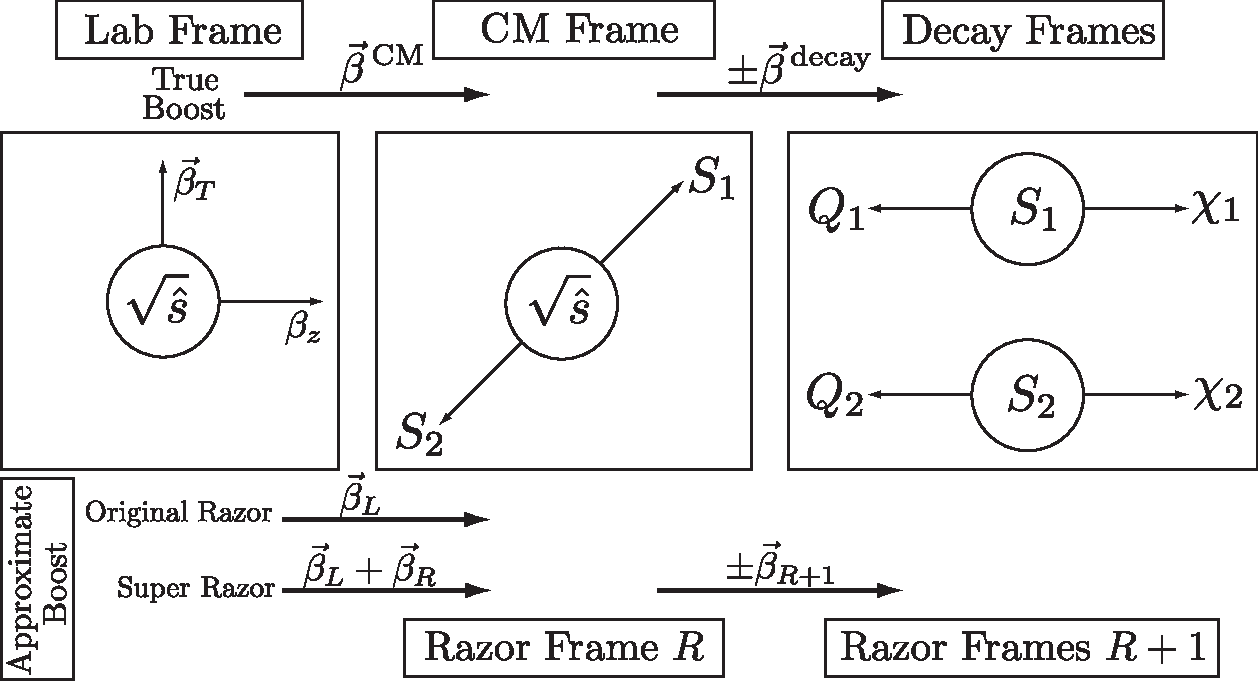
\includegraphics[width=0.9\columnwidth]{./fig/sectionII/frames2.pdf}

\caption{Sketch of the three sets of frames relevant to the razor reconstruction: the lab frame, the pair production frame for $S_1$ and $S_2$, and the two decay frames of the particles $S_i$. The approximate razor frame identified with each physically relevant frame is also shown, along with the actual and approximate boosts from one frame to the next. By convention, we label each boost by the destination frame ({\it i.e.}~boost $\vec{\beta}^{\, \rm CM}$ takes you {\it from} the lab from {\it to} the pair production center of mass frame). \label{fig:frames}}
\end{figure}

There are three kinds of frames relevant to pair production at the LHC: the lab frame, the pair production center-of-mass (CM) frame, and the two decay frames (see Figure~\ref{fig:frames}). 
The initial assumption made by the original razor construction is that the heavy parent particles are generally produced near threshold, due to the fall-off of the parton distribution functions with CM energy $\sqrt{\hat{s}}$. If we could identify the boost $\vec{\beta}^{\, \rm CM}$ from the lab frame into the $S_1$ and $S_2$ production frame (the center of mass frame CM), then this could serve as an approximation to the decay frames. We approximate this frame by making a longitudinal boost $\vec{\beta}_L$ to the razor frame $R$, which is defined here as the frame where the two sets of visible decay products $Q_1$ and $Q_2$ have equal and opposite $z$-component of momentum. This boost has magnitude
\begin{equation}
\beta_L = \frac{q_1^z+q_2^z}{E_1+E_2}. \label{eq:betaL}
\end{equation}
Here, $E_i$ is the energy of decay product $Q_i$ and $q_i^z$ is the $z$-component of the momentum.

In this razor frame, we expect $2E_{R1} \approx 2E_{R2} \approx M_\Delta$. Writing the boosted momenta in terms of lab-frame observables, we define a longitudinally boost-invariant mass
\begin{equation}
M_R^2 = (E_1+E_2)^2 - (q_1^z+q_2^z)^2. \label{eq:MR}
\end{equation}
We expect that the distribution of $M_R$ for signal events will have a peak near $M_\Delta$, assuming that our approximations of near-threshold production and $q_1^z \approx - q_2^z$ are correct on a statistical basis. Background events will not, in general, have any special feature near $M_\Delta$. For example, events consisting only of visible particles and $E_{T}^\text{miss}$ from mismeasurement would be expected to have an $M_R$ distribution proportional to the distribution of CM energy $\sqrt{\hat{s}}$, as in the case of QCD backgrounds. 

We then define a second mass variable that inherits knowledge of the mass splitting $M_\Delta$, using the visible and invisible transverse momentum in the event. Note that this information was not used in the definition of $M_R$. Motivated by the fact that backgrounds with no invisible particles must have $Q_1$ and $Q_2$ back-to-back (a fact that mismeasurement dos not tend to greatly change), we define a transverse mass in terms of the visible transverse momenta, $q_{1T}$ and $q_{2T}$, and the missing transverse energy $E_T^\text{miss}$:
\begin{equation}
(M_T^R)^2 = \frac{1}{2}\left[E_T^\text{miss} (q_{1T}+q_{2T})-\vec{E}^\text{miss}_T \cdot (\vec{q}_{1T} +\vec{q}_{2T})\right]. \label{eq:MTR}
\end{equation}
Assuming pair production at threshold, $M_T^R \leq M_\Delta$ for signal events. Introducing the dimensionless ratio
\begin{equation}
R^2 = \left(\frac{M_T^R}{M_R}\right)^2, \label{eq:R}
\end{equation}
we expect $R^2 < 1$ for signal events, with a rough spread around $R^2 \sim \tfrac{1}{4}$, while
for background without real $E_T^\text{miss}$ we expect $R\sim 0$. 
%However, selection cuts can significantly change this expectation. For example, Drell-Yan + jets dilepton %production is a primary background in the same-flavor ($e^-e^+$ and $\mu^-\mu^+$) searches we will be %considering in this paper. Requiring a reasonable amount of $E_T^\text{miss}$ (such as $E^\text{miss}_T > %60$~GeV) cuts down on this background, but also biases our sample to events where the dilepton system %recoils against an energetic jet. Mismeasurement of that jet's $p_T$ correlates the missing energy with %$\vec{q}_{1T}+\vec{q}_{2T}$, and results in a Drell-Yan background distribution with larger $R^2$.

The razor variables $M_R$ and $R^2$ were originally designed to separate QCD and other 
backgrounds from pair production of strongly-interacting heavy particles \cite{Rogan:2010kb,Chatrchyan:2011ek,CMS:2012dwa,Chatrchyan:2012gq}.\footnote{The initial use of the razor was in squark and gluino searches,
where a major background is QCD. As QCD is essentially scale-free at LHC energies, the QCD background in the razor variable $M_R$ falls exponentially. Requiring a minimum value of $R^2$, the background falls off
more and more steeply as the $R^2$ threshold is increased. This ``slicing away" of the background is the
origin of the name ``razor.''}
When used in these studies, all visible particles are assumed to fall into one of the decay chains of the parent particles $S_1$ or $S_2$. Therefore, all visible particles are assigned to a megajet $Q_1$ or $Q_2$ by a
simple algorithm, and their momenta summed. Calculation of $M_R$ and $R^2$ then proceeds as if there were only two visible objects.

\subsection{The super-razor}

Consider events that have both visible and invisible particles. Rather than splitting the visible particles into two objects $Q_1$ and $Q_2$, suppose we can divide them into three classes: particles (or groupings of particles) $Q_1$ and $Q_2$ that are assumed to come from the decay of the new physics particles $S_1$ and $S_2$, and a third class of particles that come from initial state radiation or something else extraneous to
the heavy particle decays. In electroweak production of non-colored particles, every jet in an event can be assigned to this third class. The sum of the momenta of all particles in this class is $\vec{J}$. By construction
\begin{equation}
\vec{J}_T = -\vec{E}^\text{miss}_T-\vec{q}_{1T}-\vec{q}_{2T}.
\end{equation}

The effect of $\vec{J}$ is to shift the production frame by an additional boost that was not taken into account by the original longitudinal razor boost of Eq.~\eqref{eq:betaL}. To correct for this, we want to make an additional transverse boost which takes us to the frame in which is recoiling against the jet contamination. The direction of this transverse boost is trivial: we must boost in the direction opposite to $\vec{J}$. However, there is insufficient information in the events at the LHC to unambiguously determine the magnitude of the boost. The correct boost from the lab frame to the pair production frame is
\begin{equation}
\vec{\beta}^{\, \rm CM} = \frac{\{-\vec{J}_T,p^{\, \rm CM}_z\}}{\sqrt{|\vec{J}_T|^2+(p^{\rm CM}_z)^2+\hat{s}}}, \label{eq:truelabbeta}
\end{equation}
where $p^{\rm CM}_z$ is the $z$-momentum of the center of mass frame relative to the lab frame. Neither $p^{\rm CM}_z$ or $\hat{s}$ can be determined from the available visible particle momenta at the LHC. 

We therefore must make new assumptions to build our approximate boost to the frame $R$, the razor frame that is our best guess to the pair production frame. To build this approximate boost $\vec{\beta}_R$, we make the longitudinal boost $\beta_L$, and then construct an additional boost $\vec{\beta}_R$ from approximate center of mass energy $\sqrt{\hat{s}}_R$, defining
\begin{equation}
\vec{\beta}_R = \frac{\{-\vec{J}_T,p^R_z\}}{\sqrt{|\vec{J}_T|^2+|p^R_z|^2+\hat{s}_R}}. \label{eq:razorbeta}
\end{equation}
There are two necessary assumptions to build $\hat{s}_R$. The first assumption is that the invariant mass of the visible system is equal to the invariant mass of the invisible system. This guess will result in $\hat{s}_R$ systematically lower than the actual $\hat{s}$ when the weakly interacting particles in the event are massive. Conveniently, this will actually turn out to be useful in our construction of further discriminating variables, which will be discussed shortly. The second assumption we must make is that the constructed variables (such as $\hat{s}_R$) do not depend on the unknown $p_z^R$. Clearly, this is not correct on an event-by-event basis, but allows for a determination of $\hat{s}_R$ to be made (up to a two-fold ambiguity, which we resolve by taking the positive solution). By requiring $\partial \sqrt{\hat{s}}_R/\partial p_z^R = 0$, we find (in terms of the razor variable $M_R$ of Eq.~\eqref{eq:MR})
\begin{equation}
\frac{\hat{s}_R}{4} = \frac{1}{2}\left( M_R^2 + \vec{J}_T\cdot(\vec{q}_1+\vec{q}_2) + M_R \sqrt{M_R^2+|\vec{J}_T|^2+2\vec{J}_T\cdot(\vec{q}_1+\vec{q}_2)}\right). \label{eq:hatsR}
\end{equation}
This new variable $\hat{s}_R$ can be thought of as a ``jet-corrected'' version of the original razor variable $M_R^2$ (up to a factor of four). Which is to say, it inherits information about the mass difference $M_\Delta$ and the overall pair-production energy scale $\sqrt{\hat{s}}$. 

In Figure \ref{fig:hatsMR}, we show the distributions of $M_R$ and $\sqrt{\hat{s}}_R$ (normalized to $\sqrt{\hat{s}}$) versus the $p_T$ of the CM frame, for representative slepton pair production decaying to leptons and neutralinos. As can be seen, while both $M_R$ and $\sqrt{\hat{s}}_R$ peak at the expected value given by the actual energy scale of the pair production ($\sqrt{\hat{s}}/2$ or $\sqrt{\hat{s}}$, respectively), when the center of mass is boosted to high $p_T$, the $M_R$ variable begins to show deviations from the smooth distribution. Boosting against the jets corrects for the high $p_T$ of the center of mass, as is seen in the distribution of $\sqrt{\hat{s}}_R$. The signal distributions are simulated using {\tt MadGraph5} \cite{Alwall:2011uj}, {\tt Pythia 6.4}  \cite{Sjostrand:2006za}, and {\tt PGS}; complete details of our simulations and cuts are discussed in the next section. 

\begin{figure}[ht]
%\includegraphics[width=0.32\columnwidth]{fig/sectionII/shat_v_MR.pdf}
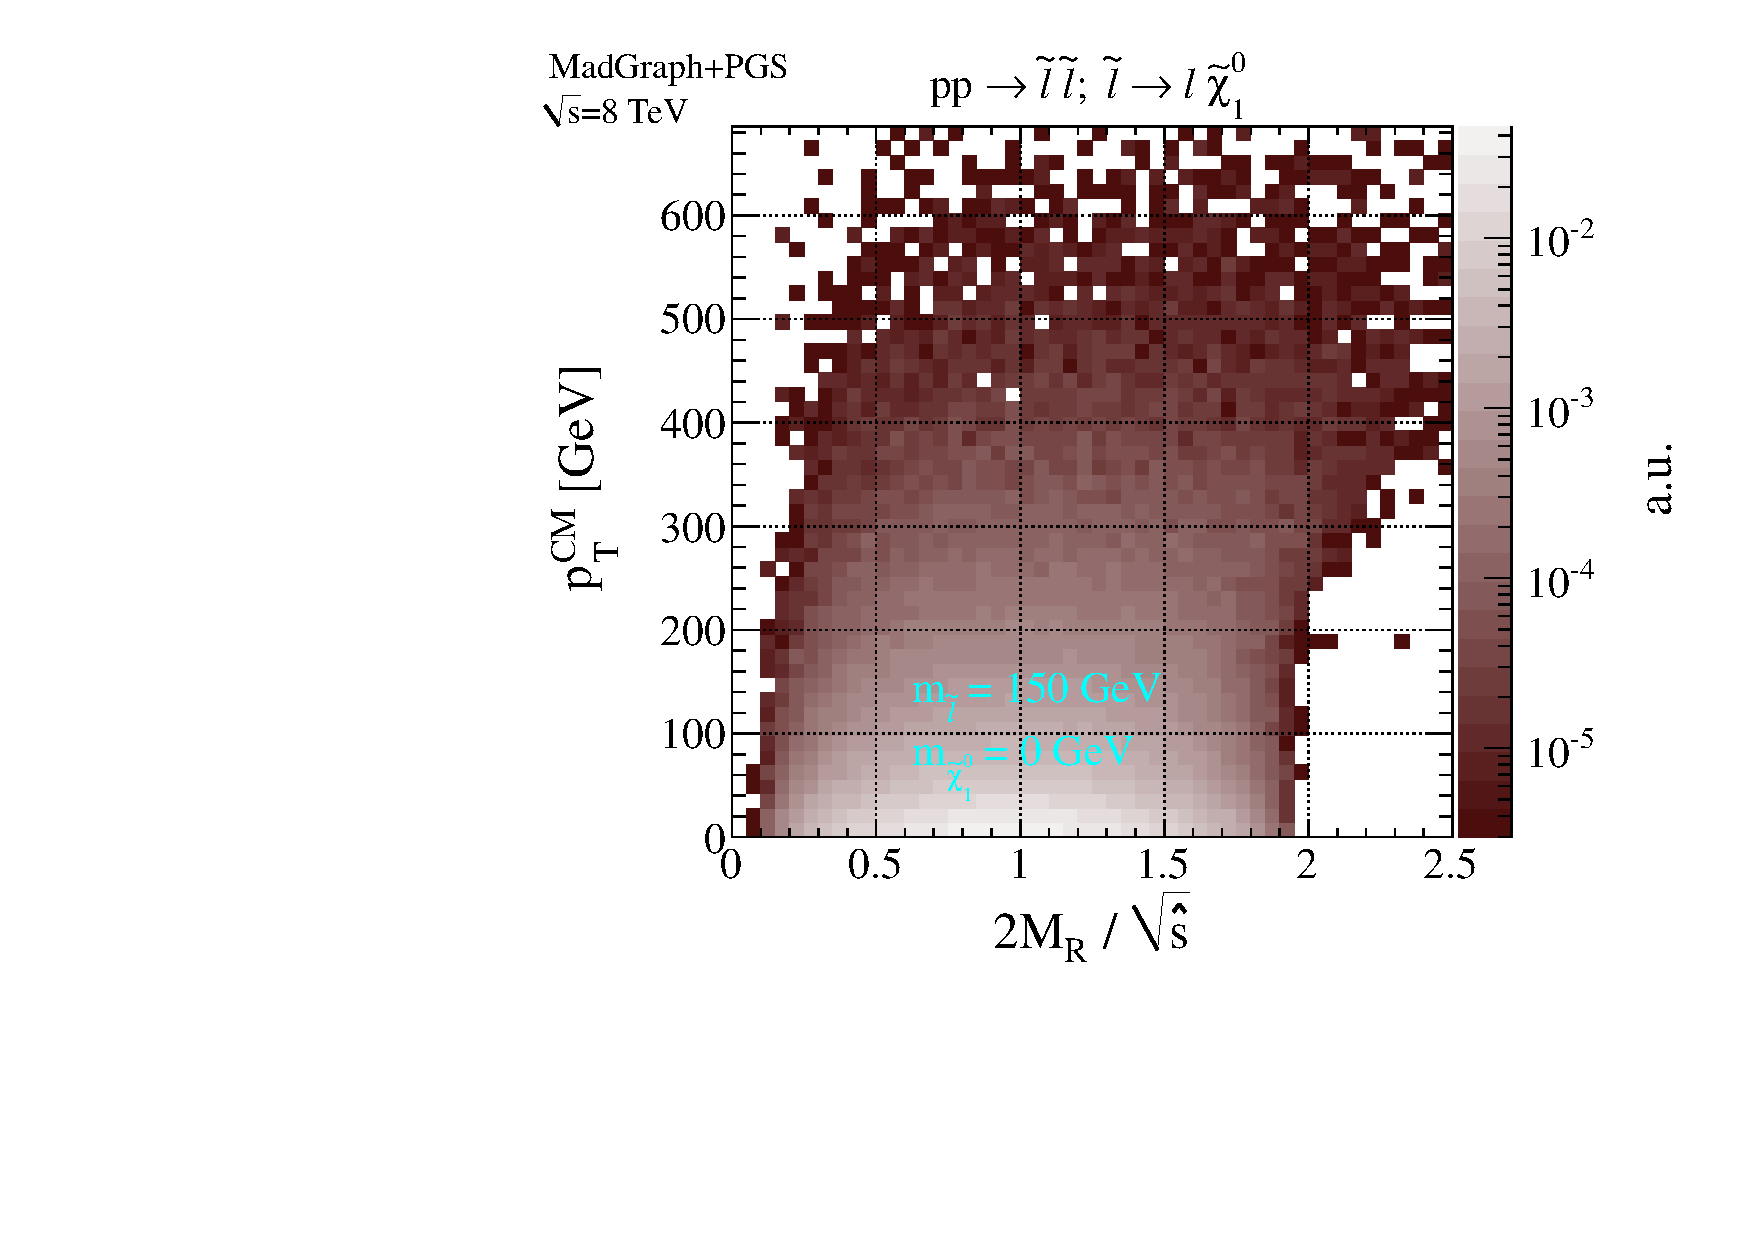
\includegraphics[width=0.4\columnwidth]{fig/sectionII/MR_norm_v_pTCM.pdf}
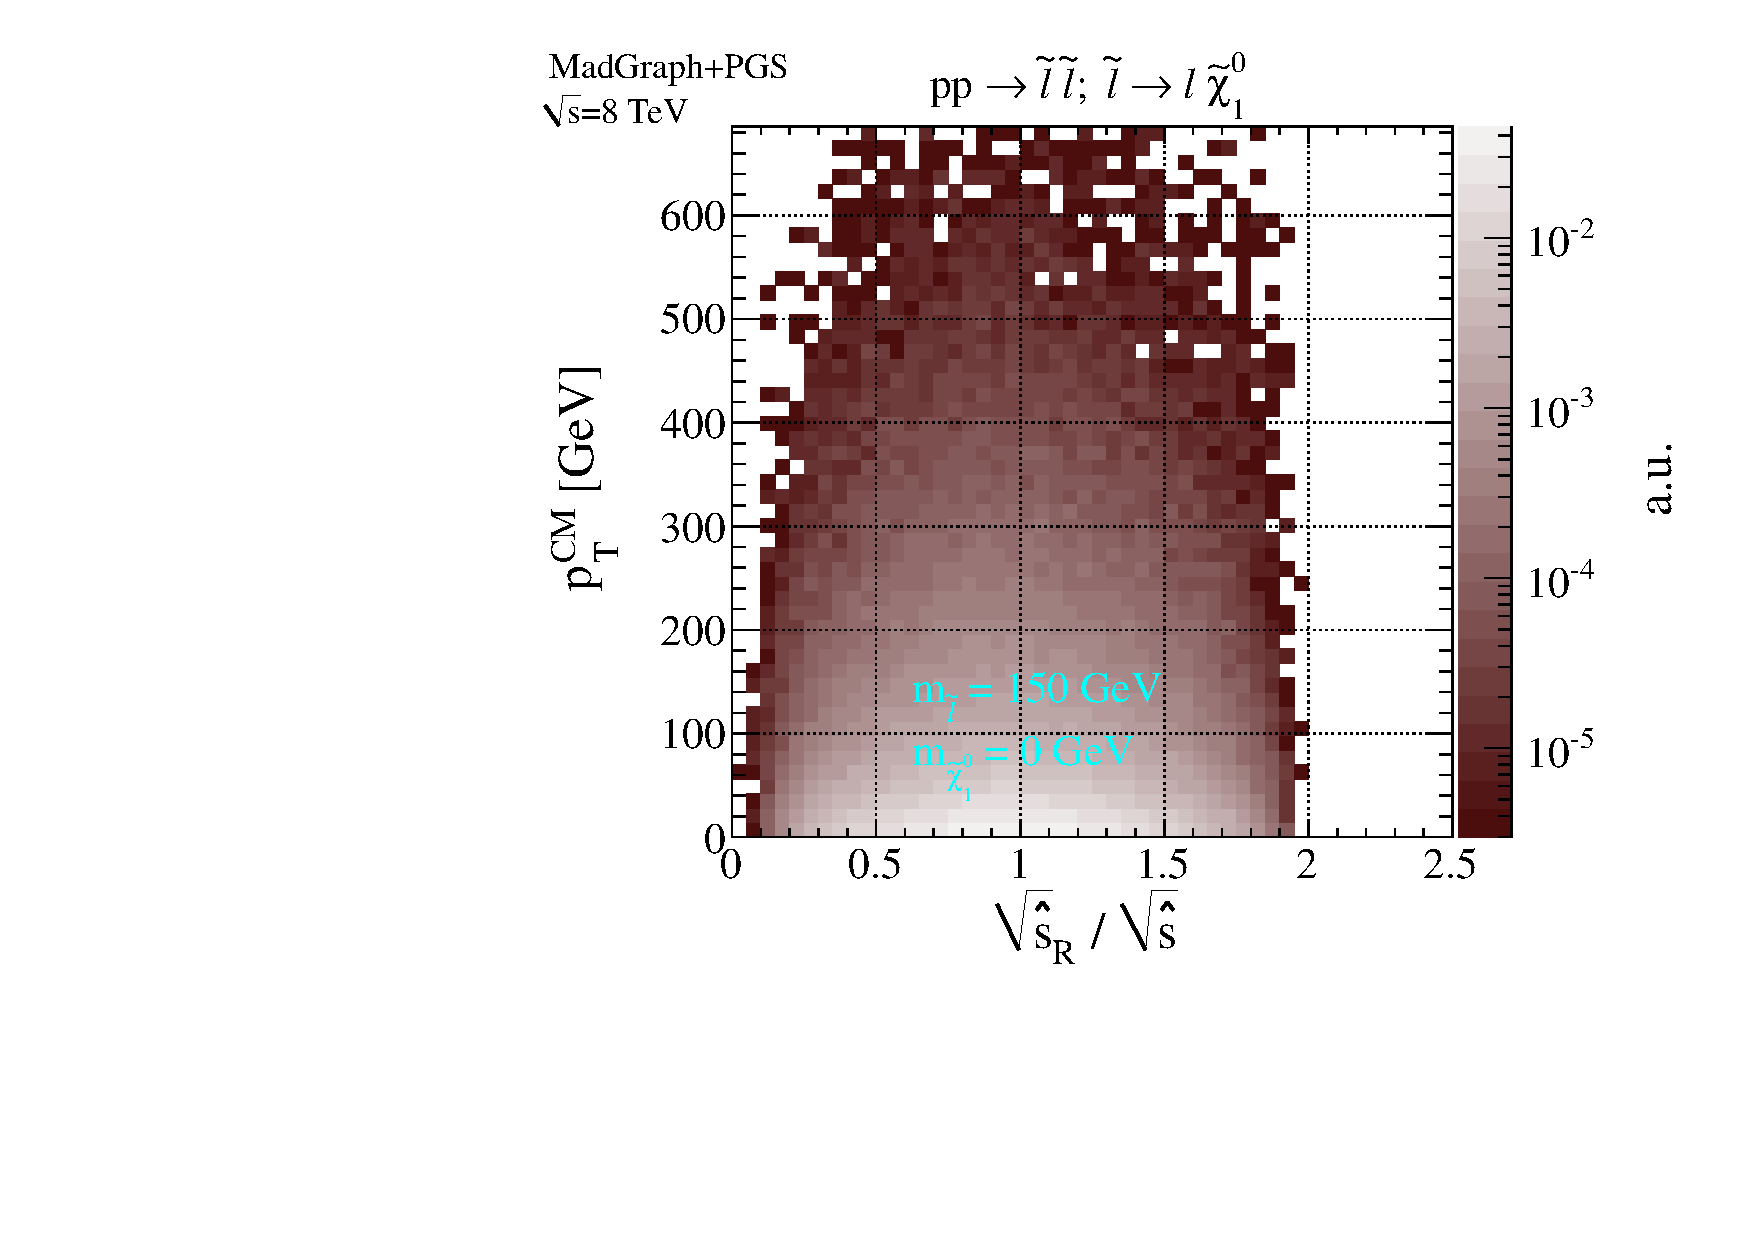
\includegraphics[width=0.4\columnwidth]{fig/sectionII/shat_norm_v_pTCM.pdf}
\caption{Distributions of razor variable $M_R$ normalized to $\sqrt{\hat{s}}$ (left) and $\sqrt{\hat{s}}_R$ normalized to $\sqrt{\hat{s}}/2$ (right) versus CM $p_T$ compared for 150~GeV slepton pair production followed by decay to leptons and massless neutralinos,. See Section~\ref{sec:simulation} for details of the simulation. \label{fig:hatsMR}}
\end{figure}

Interestingly, this variable $\hat{s}_R$ was constructed in Ref.~\cite{Rainwater:1999sd}, %called?
using a separate line of reasoning. In the razor framework, interpreting this invariant mass as the energy associated with a boost to an approximation of the pair production frame allows us to reconstruct that boost. As we will show, this leads to additional variables that add to our ability to distinguish signal and background.

Now that we are in the razor frame $R$, we can attempt to build boosts to approximations of the two decay frames of the parent particles $S_i$. Given the incomplete information available for the event, our choices for boosts are constrained. As there are two decay frames, which must have equal and opposite boosts from the pair production frame, we approximate the boost $\vec{\beta}^{~\rm decay}$ by the boost
\begin{equation}
\vec{\beta}_{R+1} = \frac{\vec{q}_{R1}-\vec{q}_{R2}}{E_{R1}+E_{R2}}, \label{eq:razorbeta1}
\end{equation}
where $q_{R1}$ and $q_{R2}$ are the 4-momenta of the two visible particles $Q_1$ and $Q_2$ in the razor frame $R$. This boost has the correct symmetry property, in that the boost to the decay frame of $S_2$ is the negative of the boost to the decay frame of $S_1$. 

If we correctly identified the boost $\vec{\beta}^{\, \rm decay}$, then the invariant mass of the pair production frame would be related to the mass of the particles $S_i$ by
\begin{equation}
\sqrt{\hat{s}} = 2 \gamma^{\rm decay}m_S.
\end{equation}
We have constructed our boosts using information from the visible system $Q_1$ and $Q_2$, so our approximate boost $\vec{\beta}_{R+1}$ and approximate CM energy $\sqrt{\hat{s}}_R$ should be related not to the mass $m_S$, but the mass difference $M_\Delta$. We therefore define a second razor variable $M_\Delta^R$,
\begin{equation}
M_\Delta^R = \frac{\sqrt{\hat{s}}_R}{2\gamma_{R+1}}, \label{eq:mdeltaR}
\end{equation}
where $\gamma_{R+1}$ is the Lorentz factor associated with the boosts $\vec{\beta}_{R+1}$. This variable should approximate $M_\Delta$ for signal events.

Clearly, building these razor frames requires many assumptions, approximations, and choices that may appear to be {\it ad hoc}. We take the attitude that this technique is justified if, in the end, we find variables that well-approximate the true  values.  In Figure~\ref{fig:beta}, we plot the distributions of $\beta_R$ for both the primary $W^-W^+$ background and slepton or chargino signal production, in all cases decaying to two charged leptons and missing energy. We also plot the boosts $\beta_R$ normalized to the true transverse boost to the CM frame $\beta^{\, \rm CM}_T$.  The equivalent plots for $\beta_{R+1}$ (including normalization to $\beta^{\, \rm decay}$) are shown in Figure~\ref{fig:betap1}.

As expected for a proton-proton collider, the distributions of signal and background events all tend towards small boosts. For signal events, we see that we are systematically overestimating -- albeit slightly -- the magnitude of the boost $\beta_R$ as compared to the true value $\beta^{\, \rm CM}_T$ . This effect is more pronounced when the splitting between the parent and daughter is small. We also mis-estimate the boost by a larger amount for charginos as compared to sleptons. This makes sense, as in constructing $\sqrt{\hat{s}}_R$, we made the assumption that the visible and invisible invariant masses are equal. This becomes increasingly incorrect as the invisible system's mass increases. The presence of extra invisible particles (neutrinos) in the chargino decays also will systematically skew that measurement. We will shortly take advantage of these systematic differences between the mass of the invisible system in the background and signal events to increase our discrimination power using a new set of variables. 

\begin{figure}[ht]
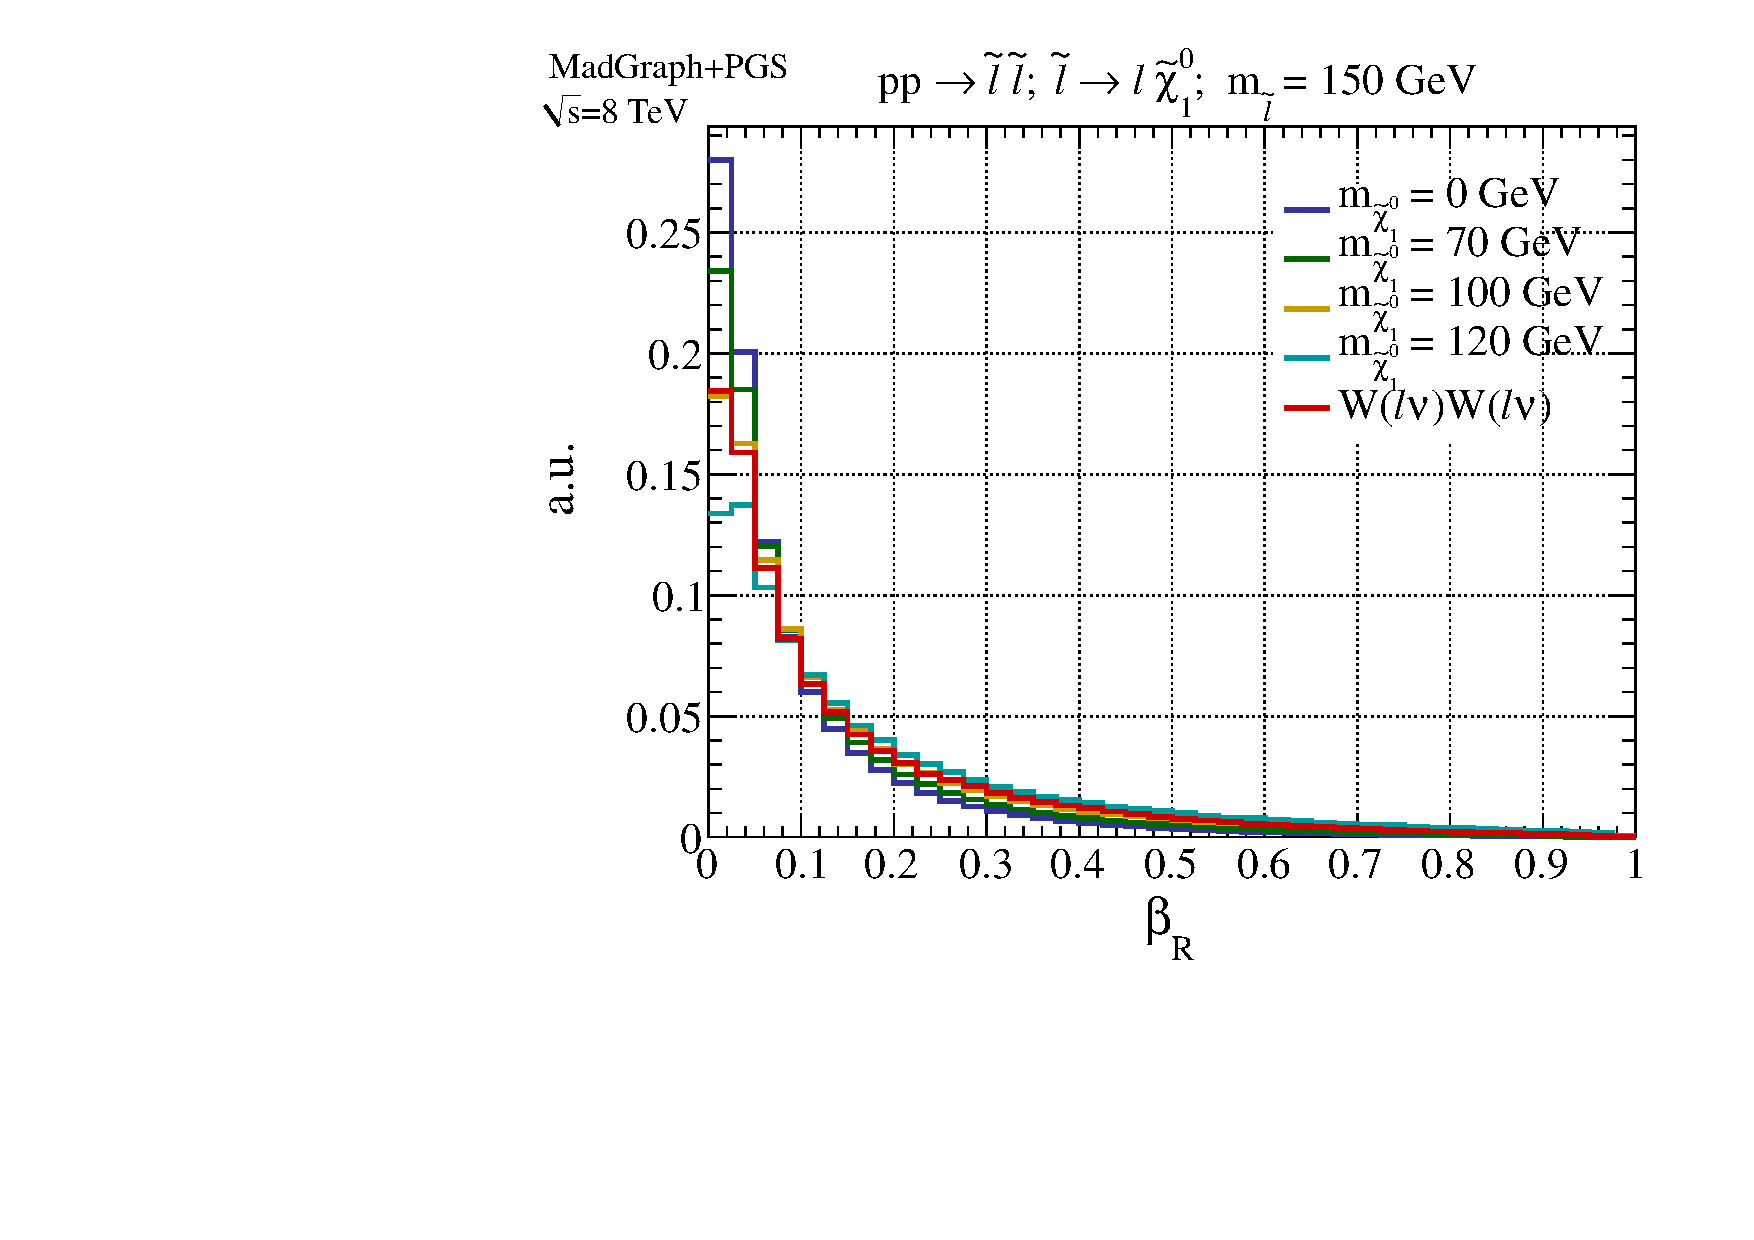
\includegraphics[width=0.4\columnwidth]{fig/sectionII/betaR_1D_slepton.pdf}
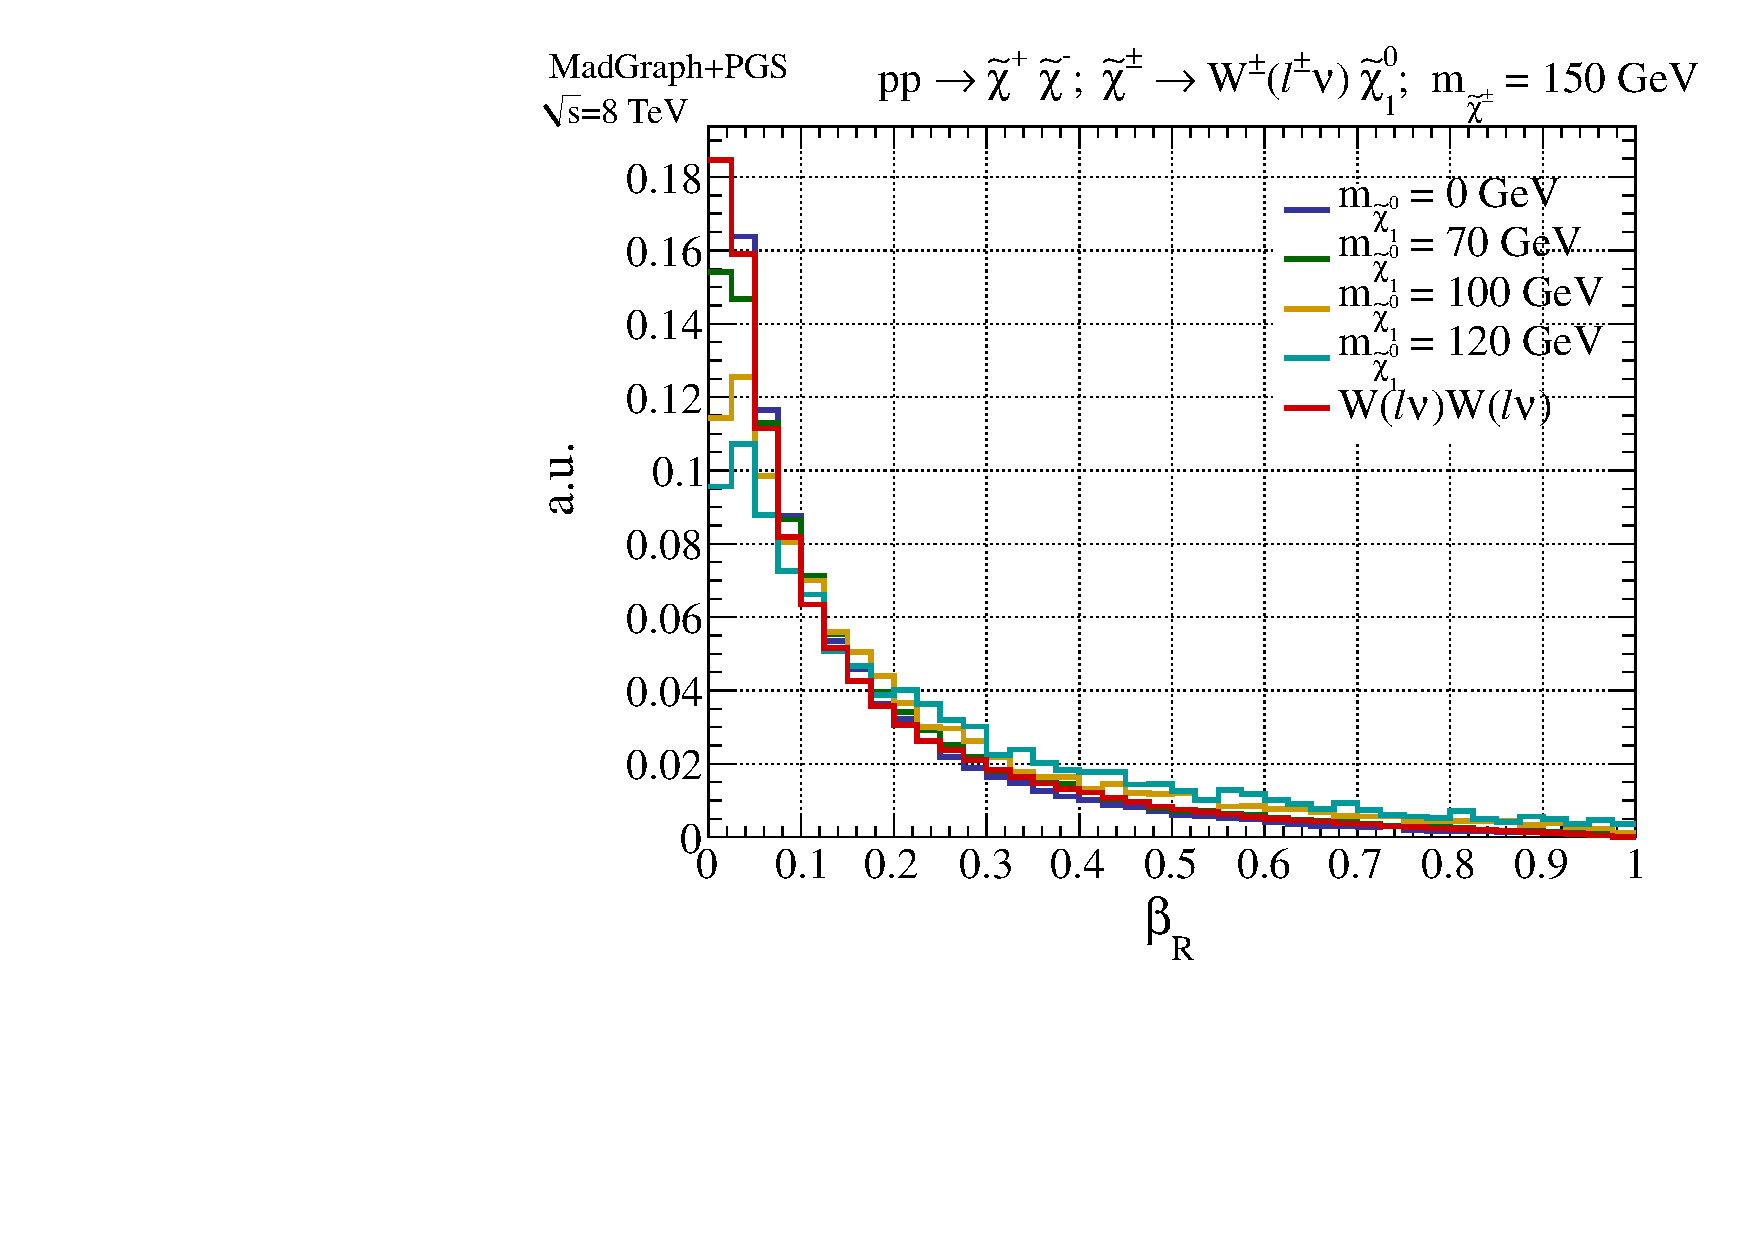
\includegraphics[width=0.4\columnwidth]{fig/sectionII/betaR_1D_chargino.pdf}
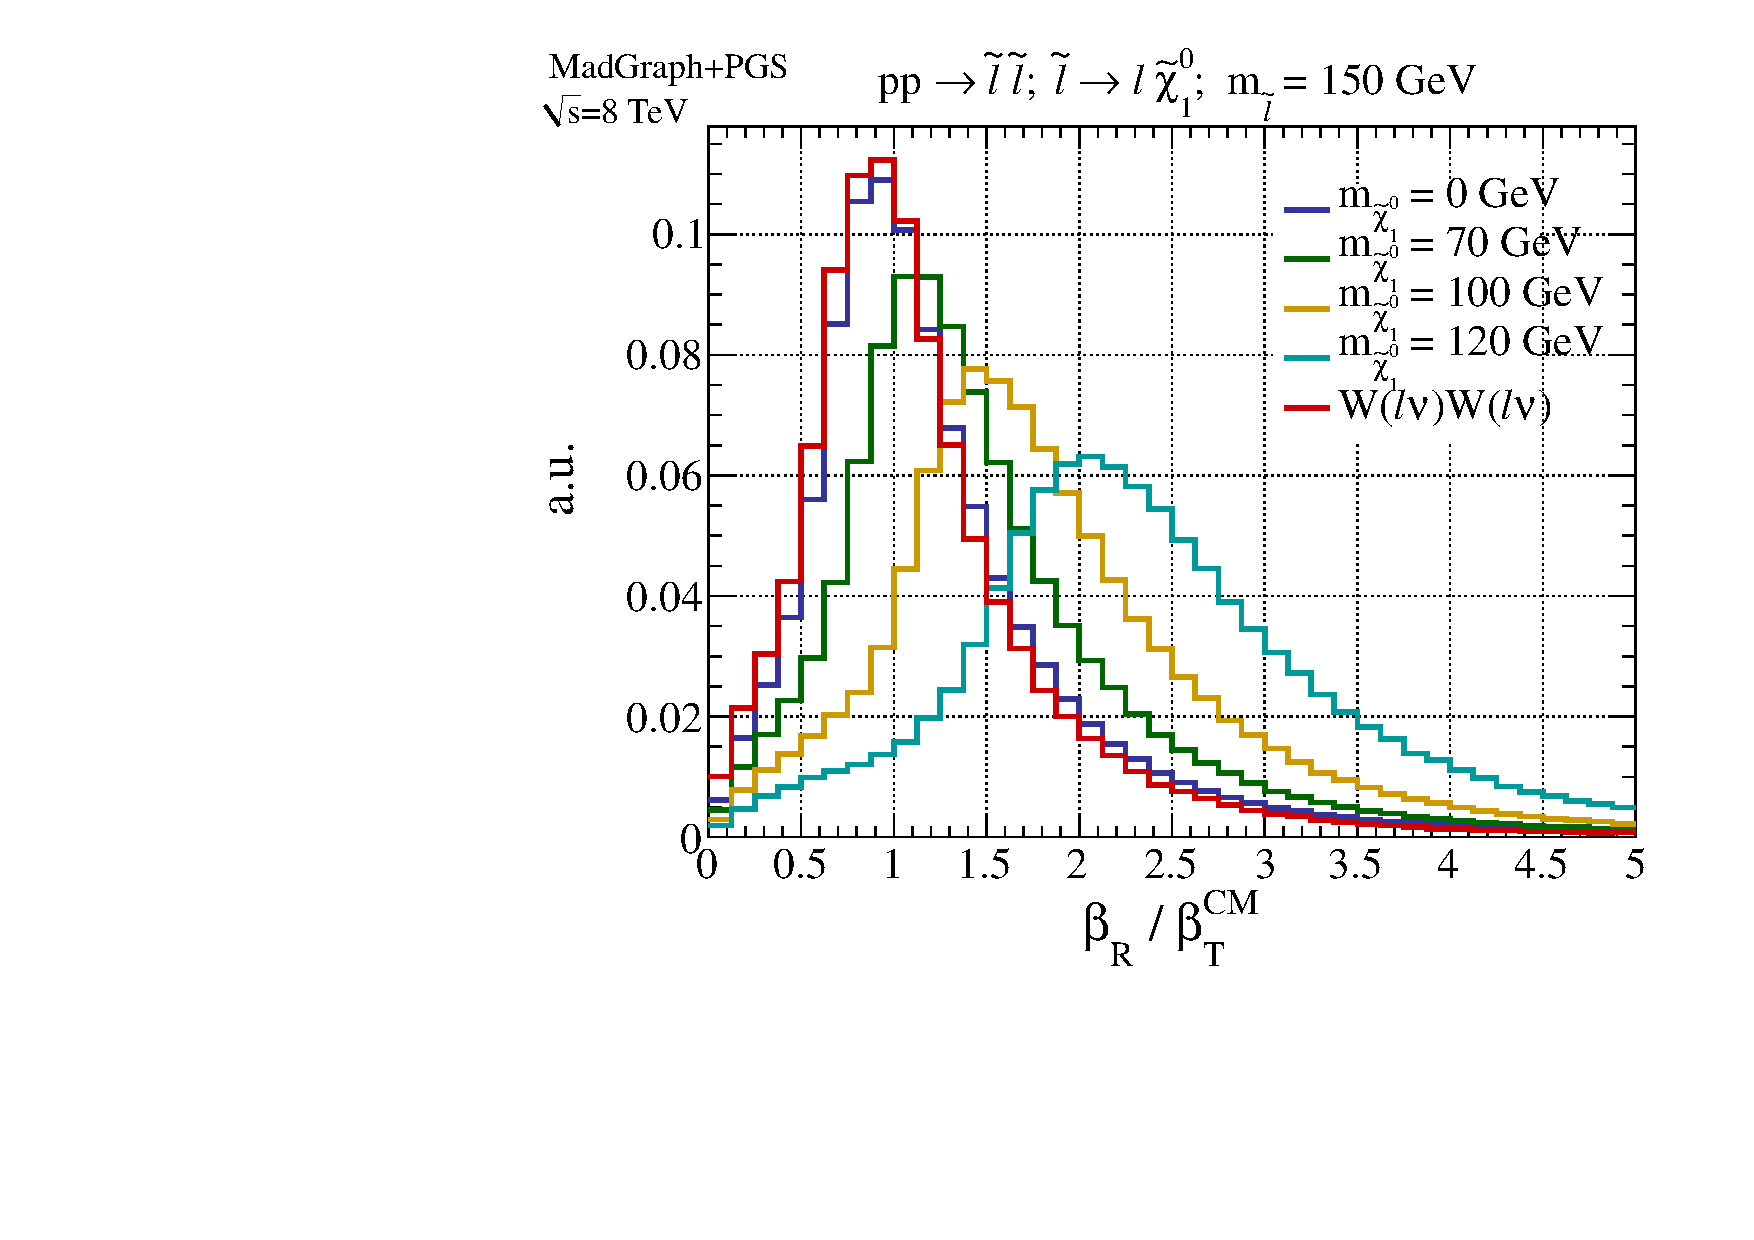
\includegraphics[width=0.4\columnwidth]{fig/sectionII/betaR_norm_1D_slepton.pdf}
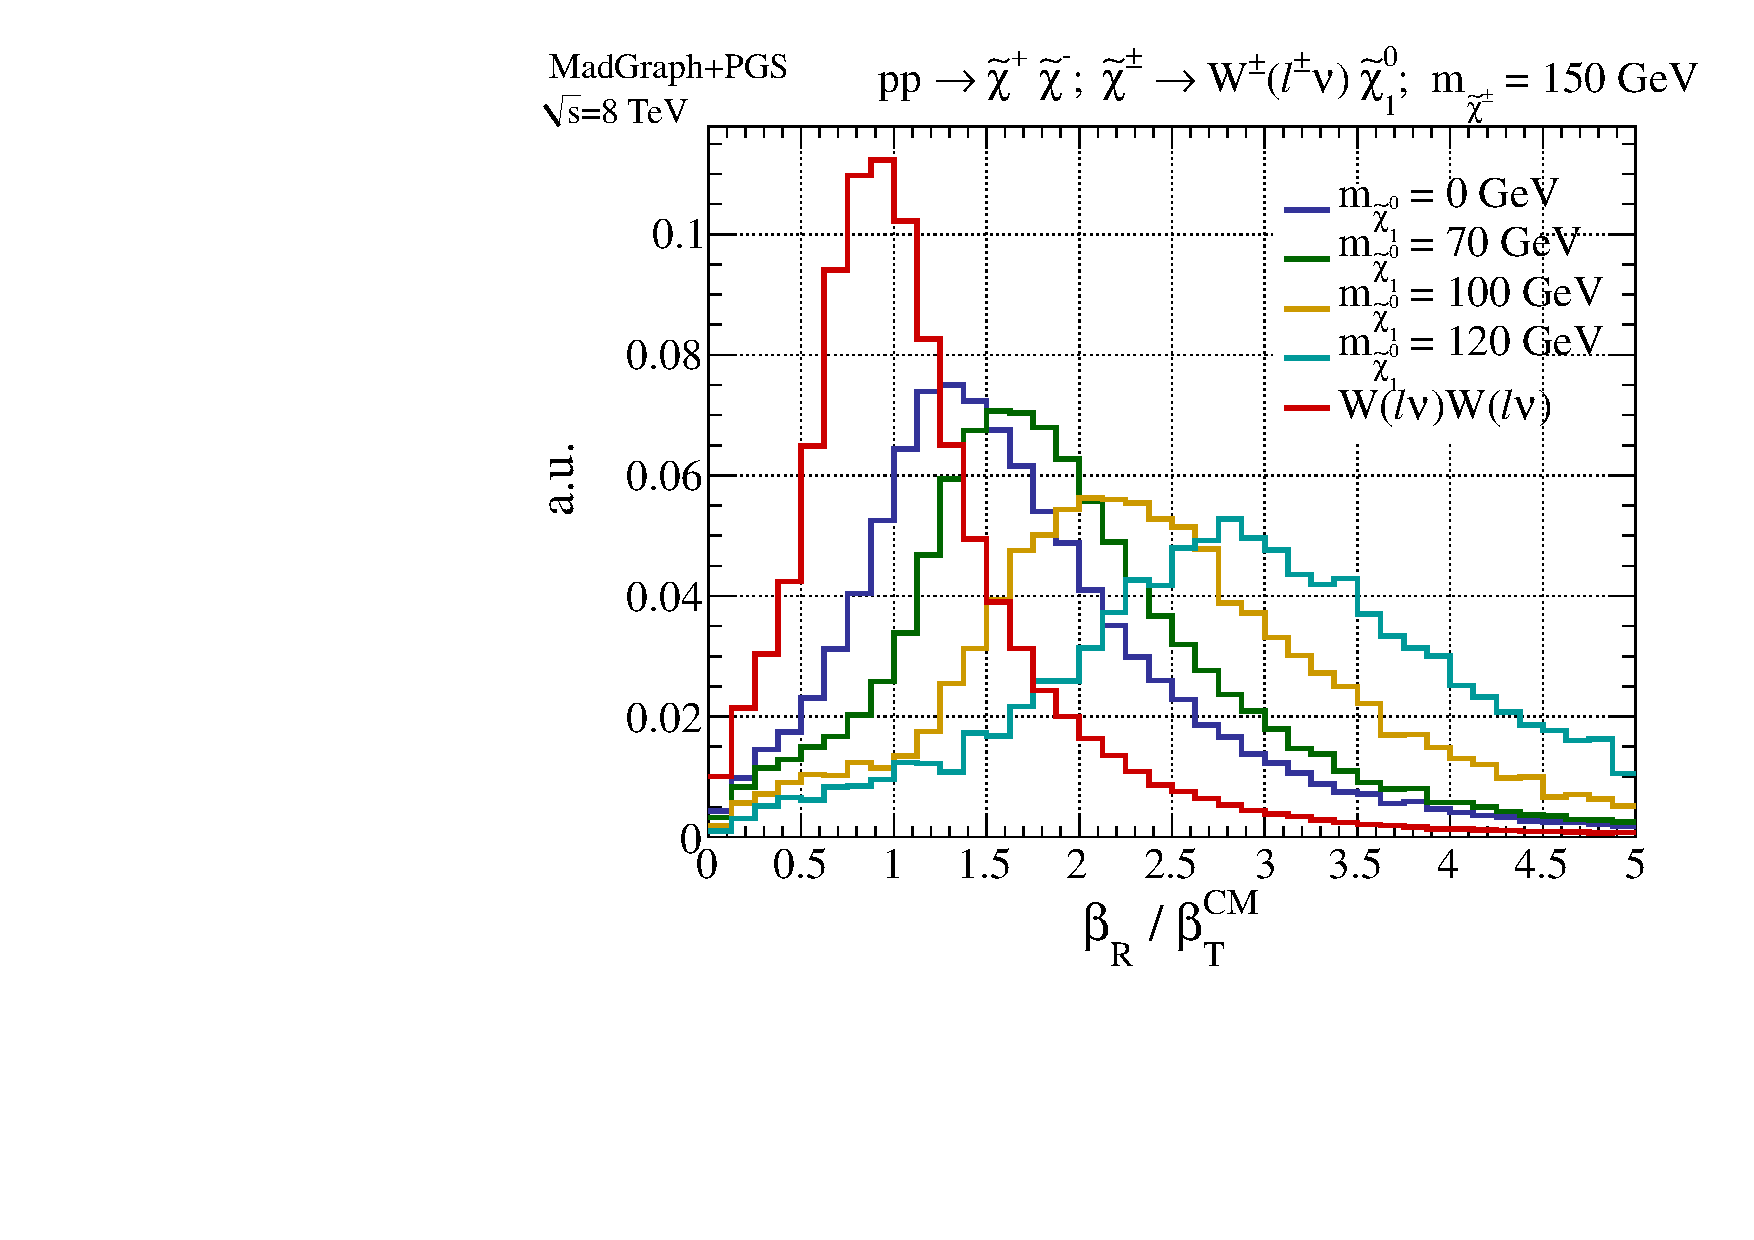
\includegraphics[width=0.4\columnwidth]{fig/sectionII/betaR_norm_1D_chargino.pdf}

\caption{Top Row: Distributions of $\beta_R$ for 150~GeV selectrons (left) or charginos (right) decaying into neutralinos and electrons, for a range of neutralino masses. Also shown is the distribution of the $W^-W^+$ background. Bottom Row: Distributions of normalized $\beta_R/\beta_T^{\, \rm CM}$ (right) for 150~GeV selectrons (left) or charginos (right) decaying into neutralinos, again for a range of neutralino masses. \label{fig:beta}}
\end{figure}

\begin{figure}[ht]
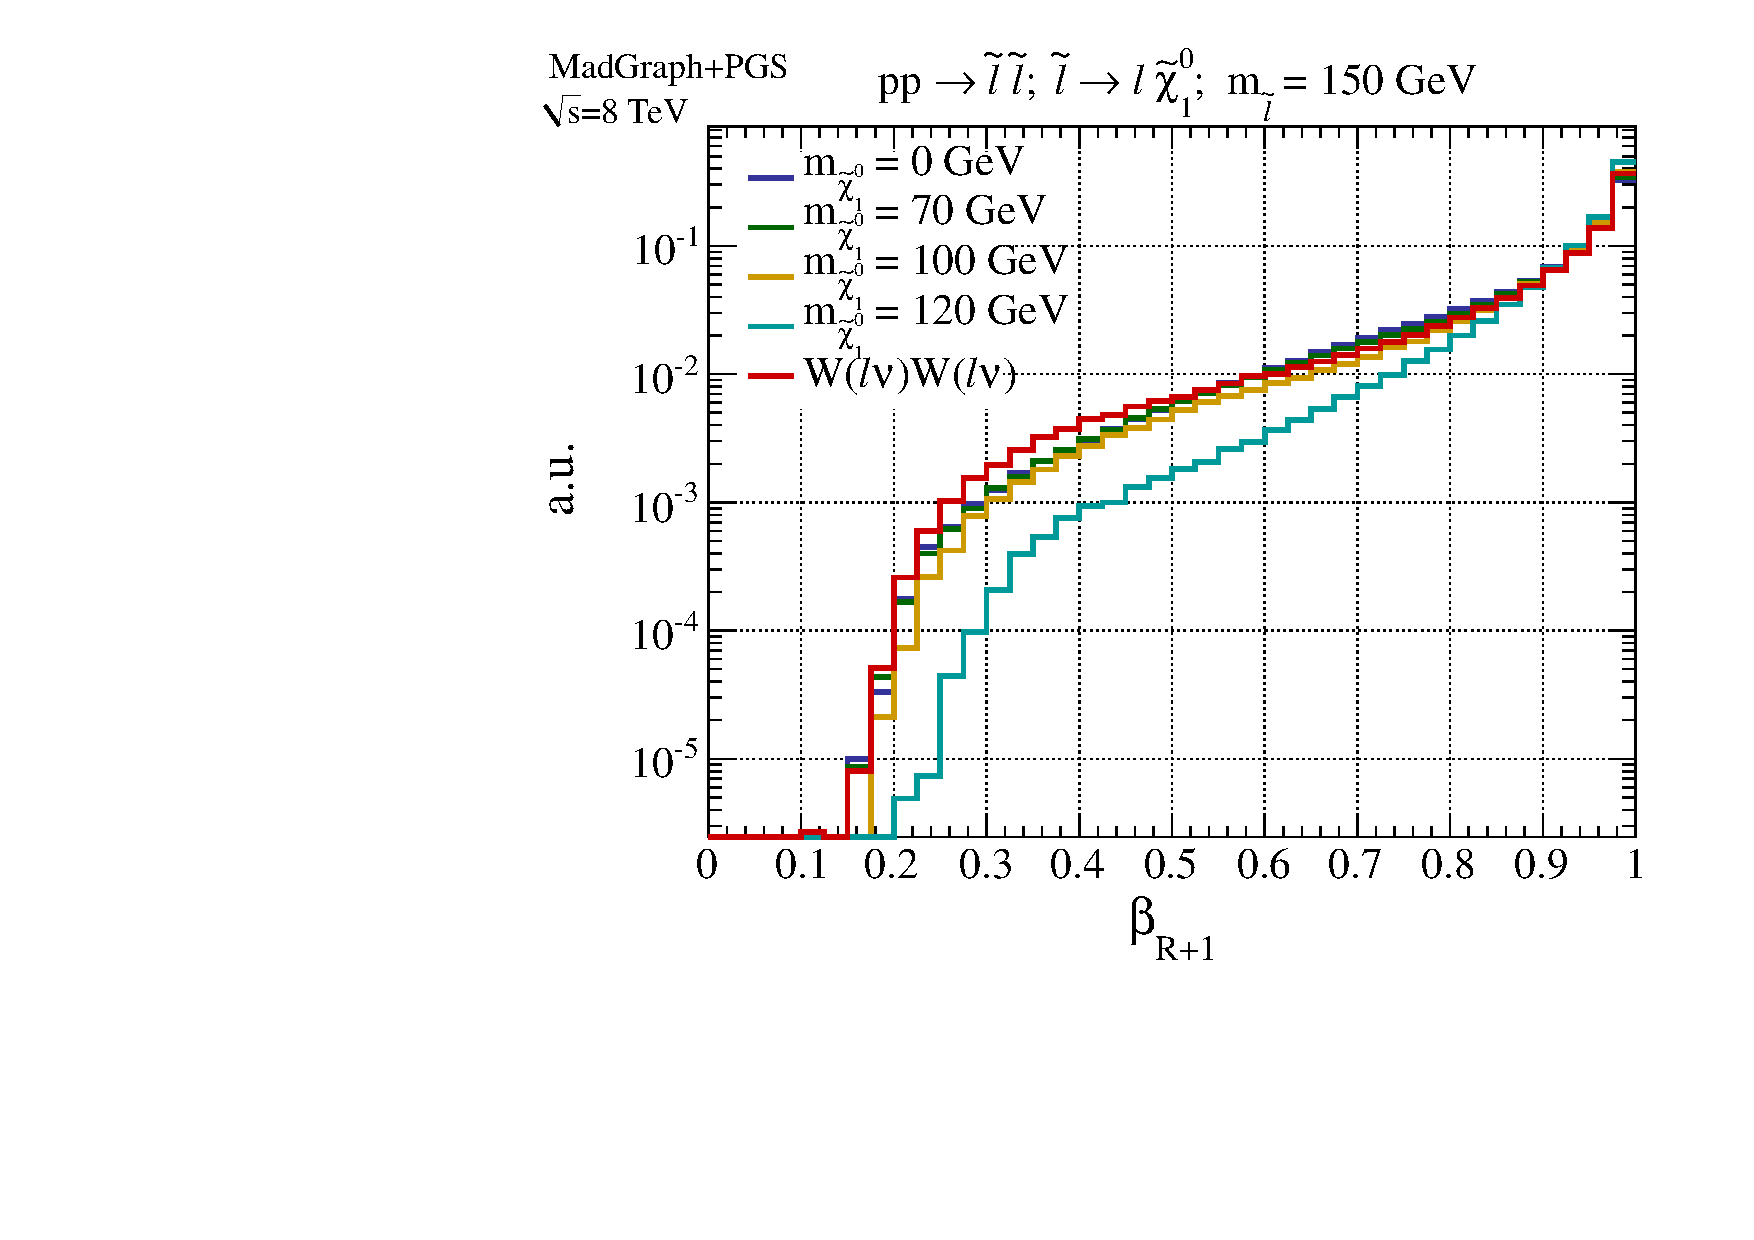
\includegraphics[width=0.4\columnwidth]{fig/sectionII/betaRp1_1D_slepton.pdf}
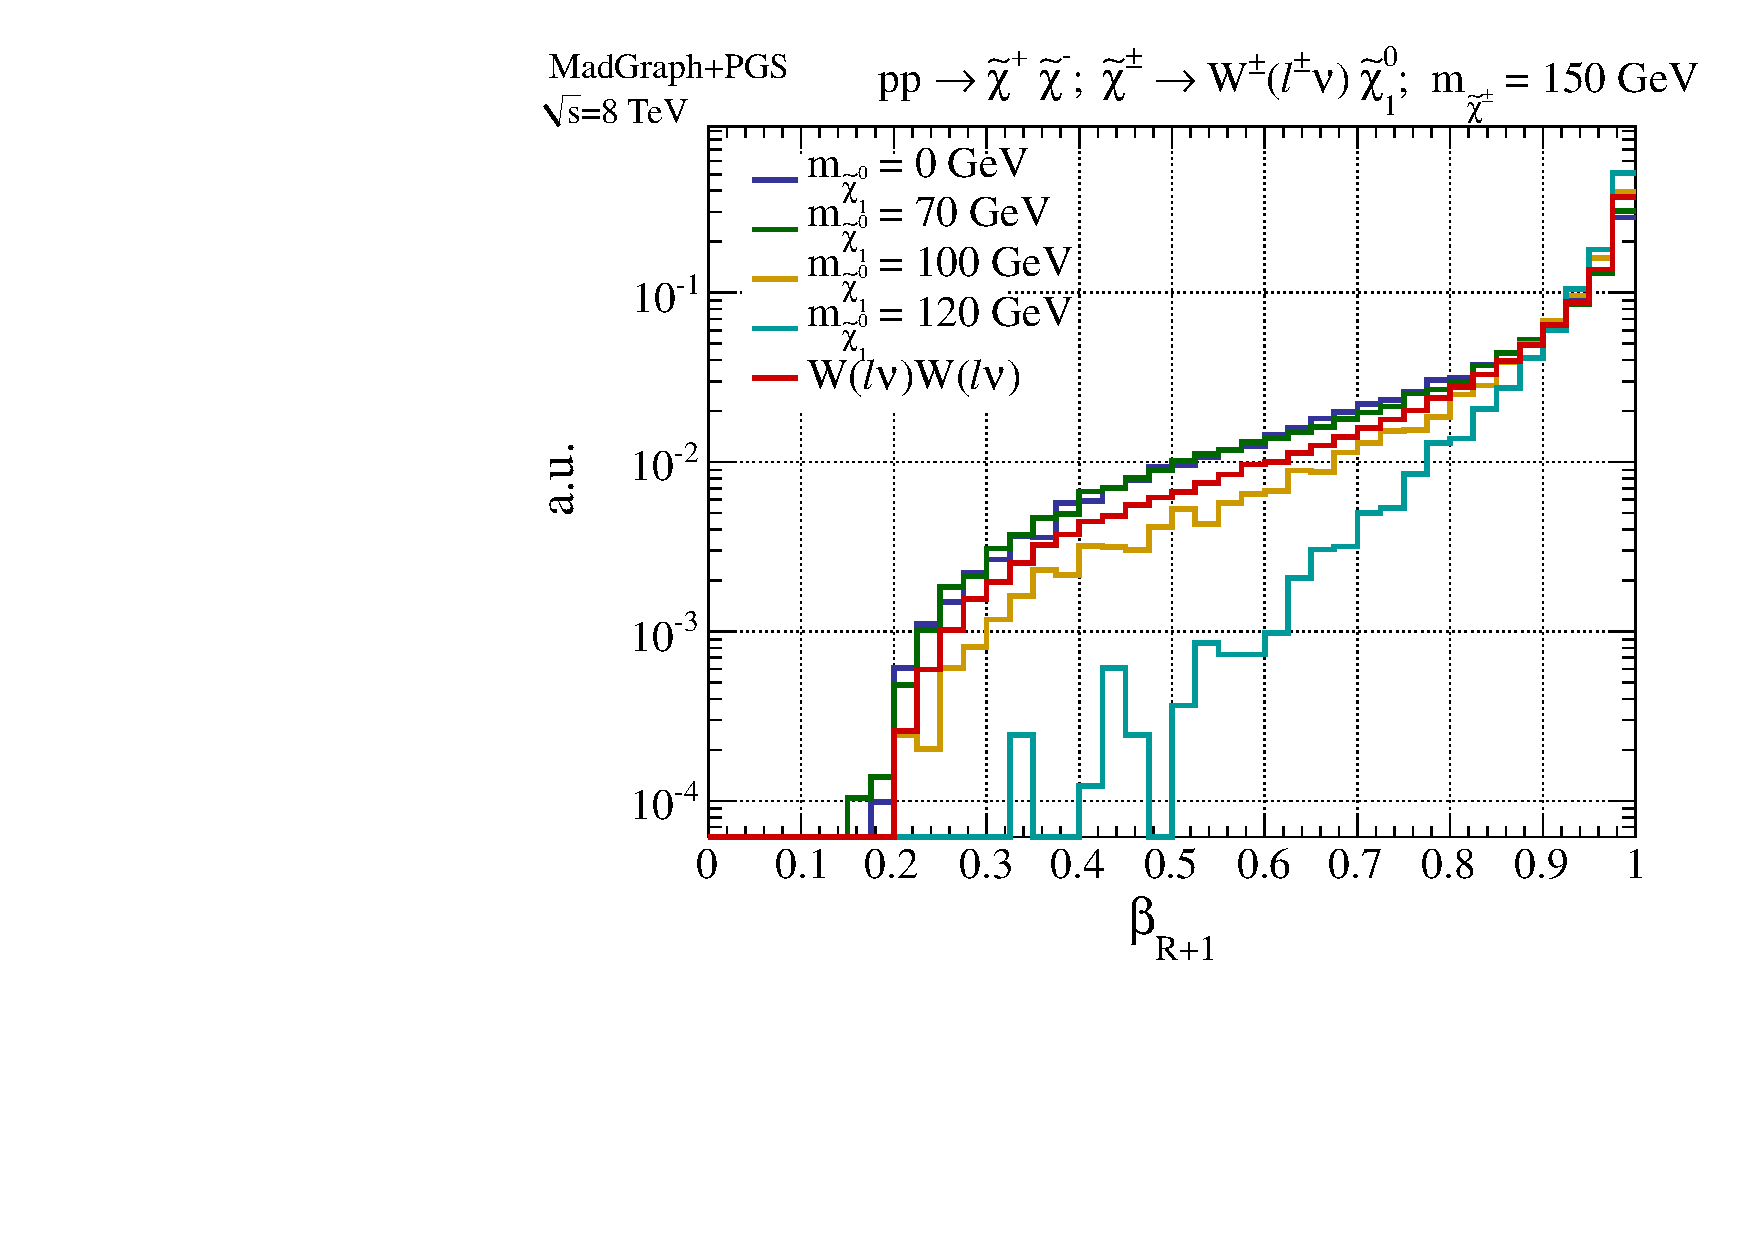
\includegraphics[width=0.4\columnwidth]{fig/sectionII/betaRp1_1D_chargino.pdf}
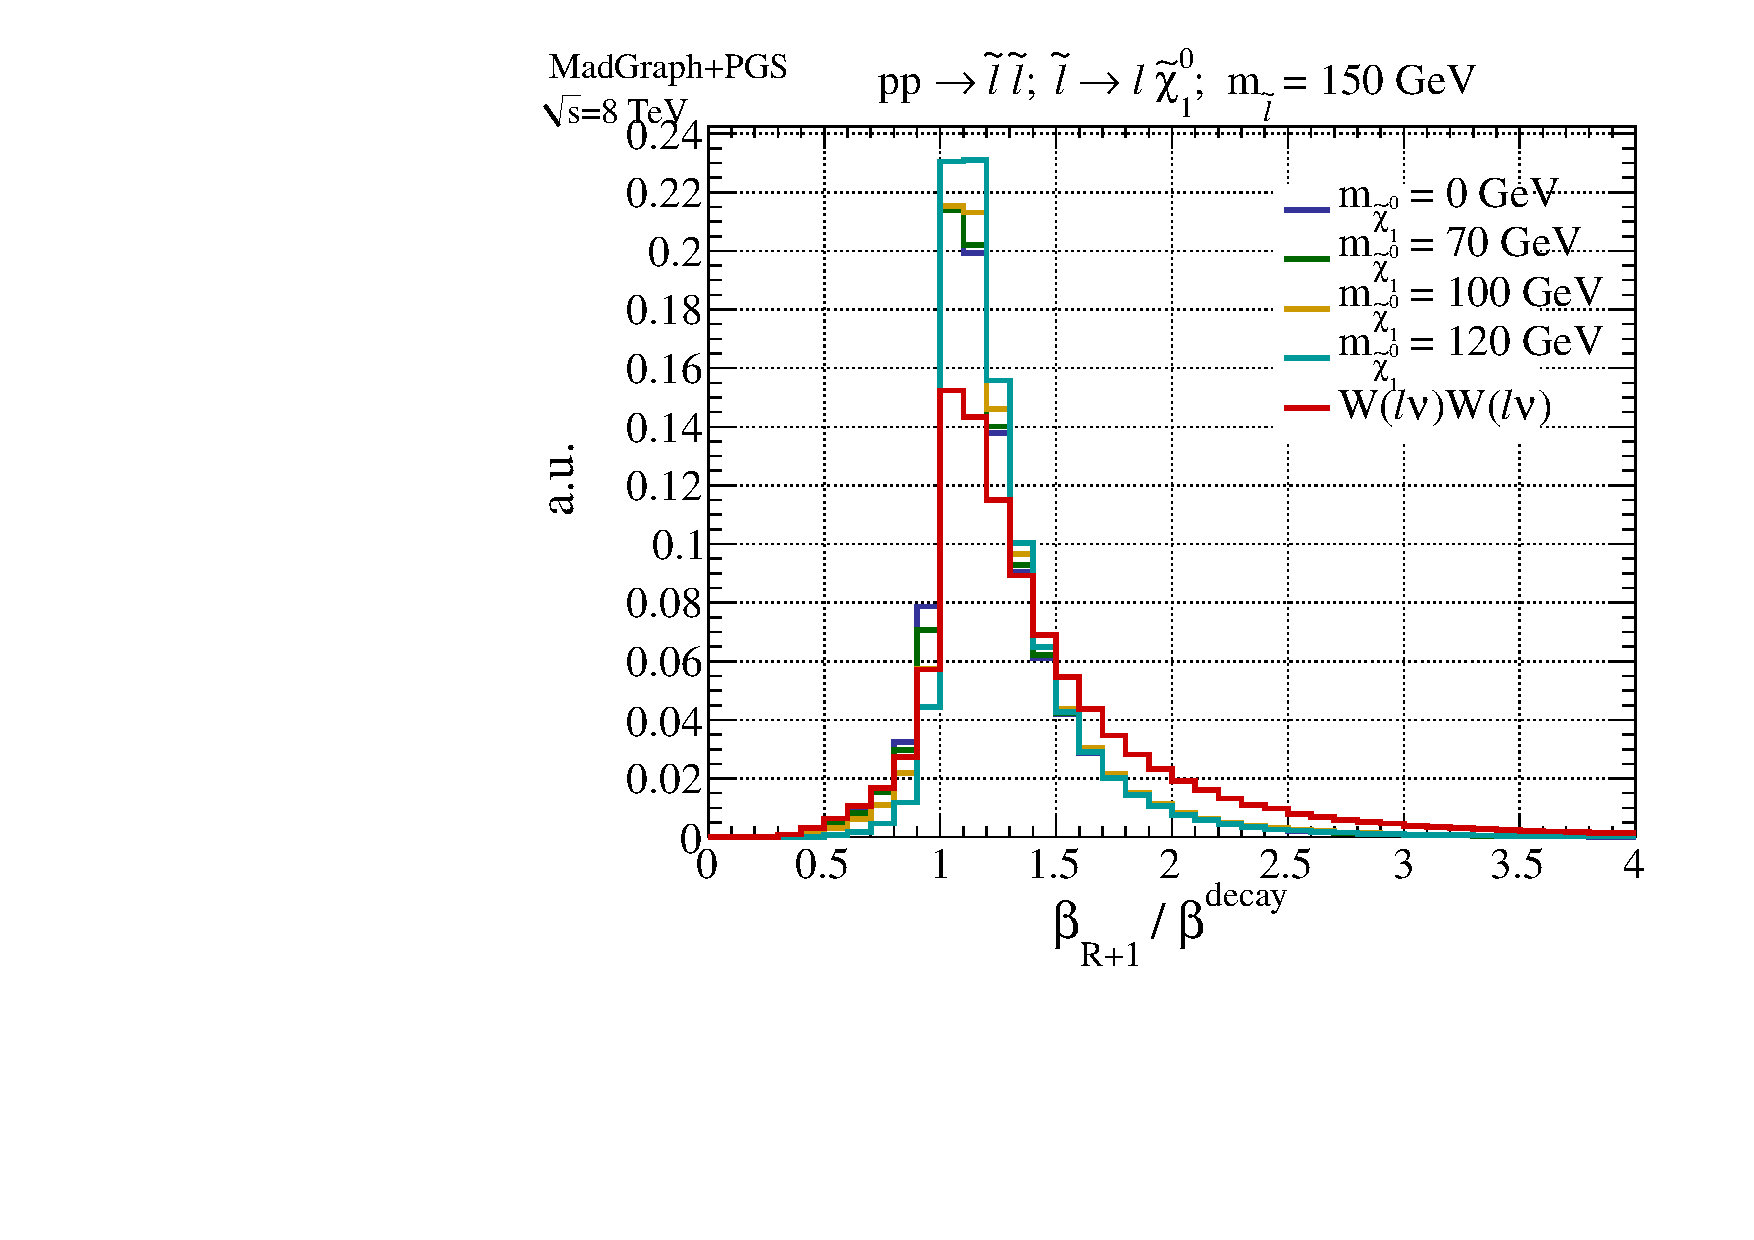
\includegraphics[width=0.4\columnwidth]{fig/sectionII/betaRp1_norm_1D_slepton.pdf}
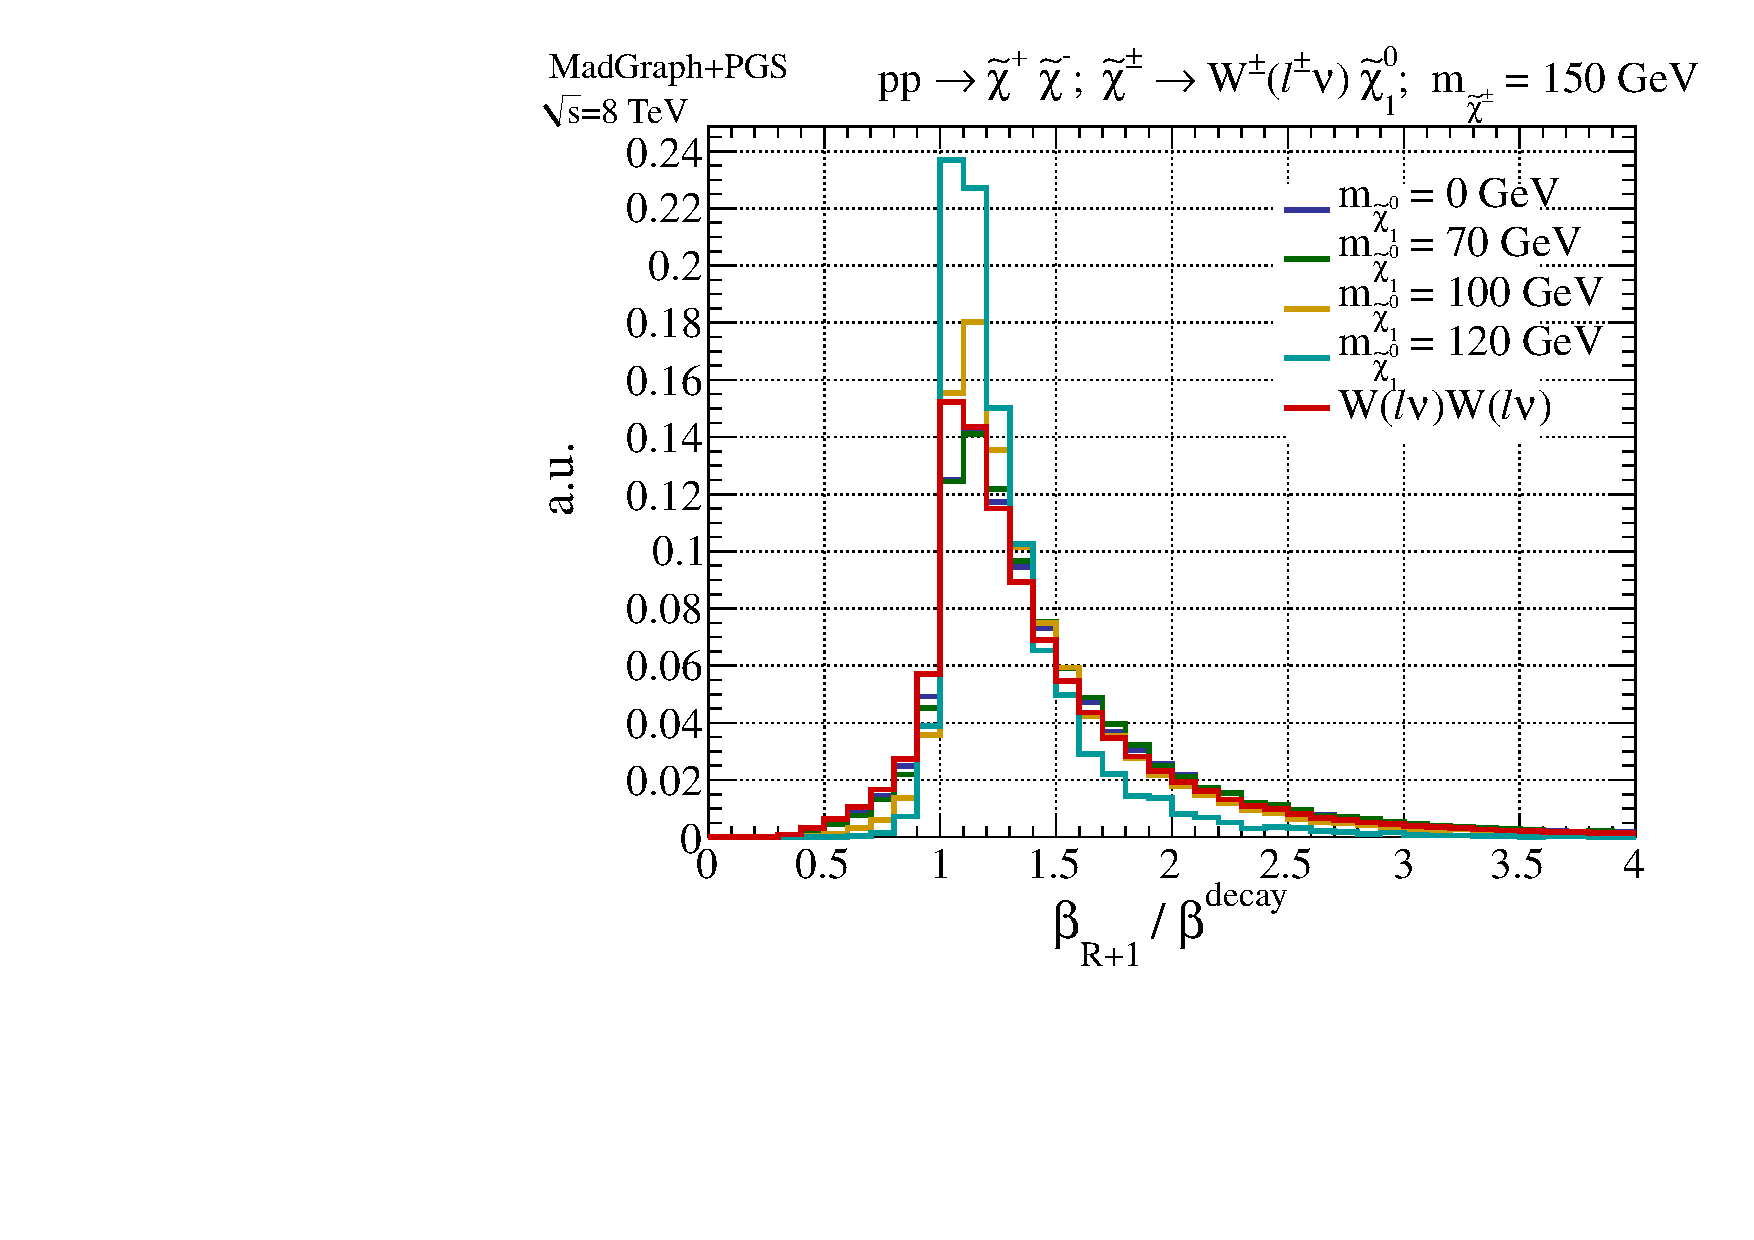
\includegraphics[width=0.4\columnwidth]{fig/sectionII/betaRp1_norm_1D_chargino.pdf}
\caption{Top Row: Distributions of $\beta_{R+1}$ for 150~GeV selectrons (left) or charginos (right) decaying into neutralinos and electrons, for a range of neutralino masses. Also shown is the distribution of the $W^-W^+$ background. Bottom Row: Distributions of normalized $\beta_{R+1}/\beta^{\, \rm decay}$ (right) for 150~GeV selectrons (left) or charginos (right) decaying into neutralinos, again for a range of neutralino masses. \label{fig:betap1}}
\end{figure}

%\begin{figure}[ht]
%\includegraphics[width=0.32\columnwidth]{fig/sectionII/betaCM_true_v_betaR_slepton_150_0.pdf}
%\includegraphics[width=0.32\columnwidth]{fig/sectionII/betaCM_true_v_betaR_slepton_150_100.pdf}
%\includegraphics[width=0.32\columnwidth]{fig/sectionII/betaCM_true_v_betaR_WW.pdf}
%\includegraphics[width=0.32\columnwidth]{fig/sectionII/betaCM_true_v_betaR_chargino_150_0.pdf}
%\includegraphics[width=0.32\columnwidth]{fig/sectionII/betaCM_true_v_betaR_chargino_150_100.pdf}
%\caption{Top Row: distributions of $\gamma_{R}$ for a range of $(m_{\tilde{e}},m_{\tilde{\chi}})$ signal points (right), and distributions of $\gamma_{R+1}$ (right). \\
%Bottom Row: distributions of $\gamma_R$ normalized to $\gamma^{\rm CM}$ (left), and distributions of $\gamma_{R+1}$ normalized to $\gamma^{\rm decay}$ (right).  \label{fig:compare_razor1}}
%\end{figure}

In Figure~\ref{fig:compare_hats} we plot the distributions of $\sqrt{\hat{s}}_R$ for a range of signal points and the $W^-W^+$ background, as well as the ratio of this razor variable to the quantity it is intended to estimate, $2\gamma^{\rm decay}M_\Delta$ (for background, the splitting $M_\Delta$ is the $W$ boson mass $m_W$, as the neutrino is massless for our purposes). As can be seen, the razor approximation is reasonably good, though systematically low for signal points with massive neutralinos, and less accurate for charginos than sleptons, for the reasons discussed previously. In Figure~\ref{fig:compare_mdelta}, we plot the distributions of the variable $M_\Delta^R$, both by itself and normalized to the estimator value of $M_\Delta$. The sharp edge at $M_\Delta^R = M_\Delta$ (seen most clearly in the slepton plot) indicates that this variable is useful in searches for new physics, especially in the regime where $M_\Delta$ is greater than the mass of the $W$ boson.

%\begin{figure}[ht]
%\includegraphics[width=0.32\columnwidth]{fig/sectionII/Mdelta_norm_v_shat_normtrue_chargino_150_0.pdf}
%\includegraphics[width=0.32\columnwidth]{fig/sectionII/Mdelta_norm_v_shat_normtrue_chargino_150_50.pdf}
%\includegraphics[width=0.32\columnwidth]{fig/sectionII/Mdelta_norm_v_shat_normtrue_chargino_150_100.pdf}
%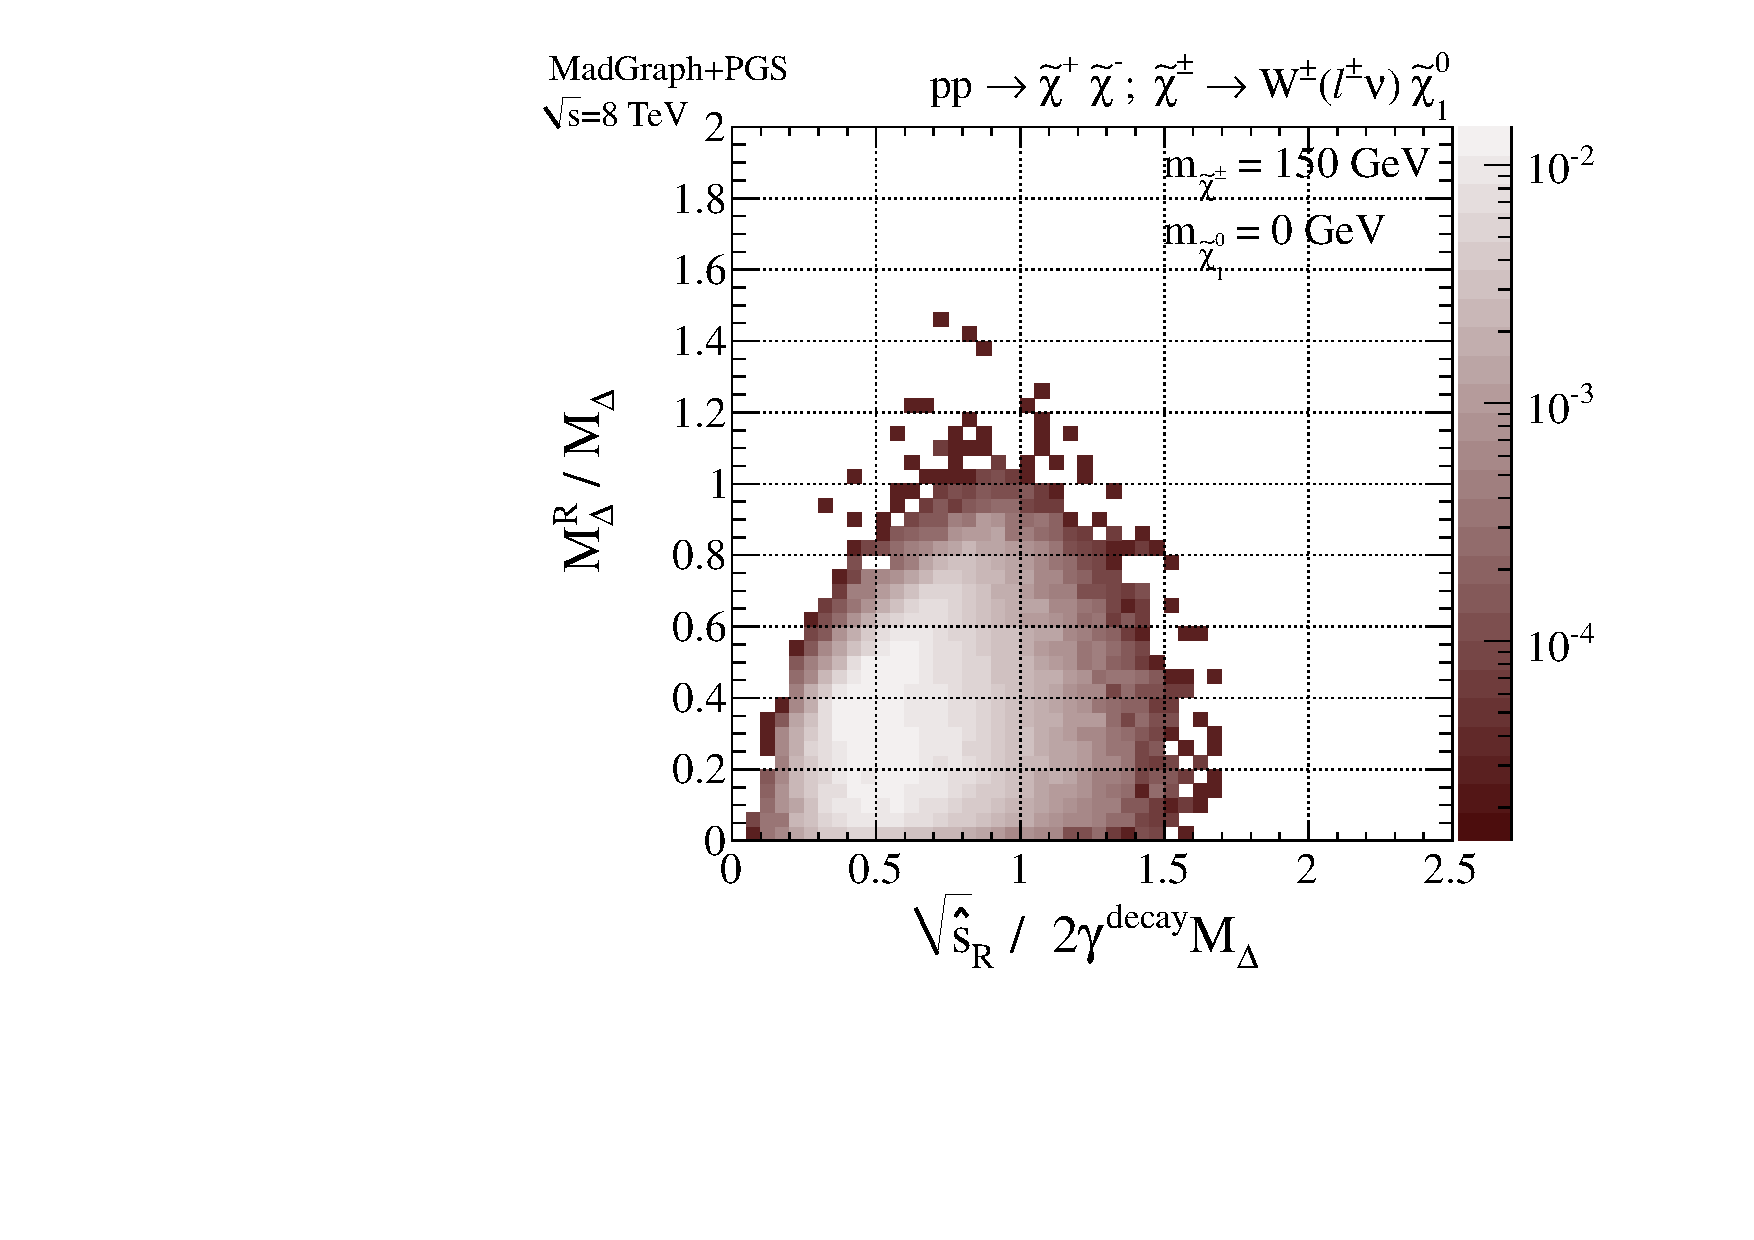
\includegraphics[width=0.32\columnwidth]{fig/sectionII/Mdelta_norm_v_shat_norm_chargino_150_0.pdf}
%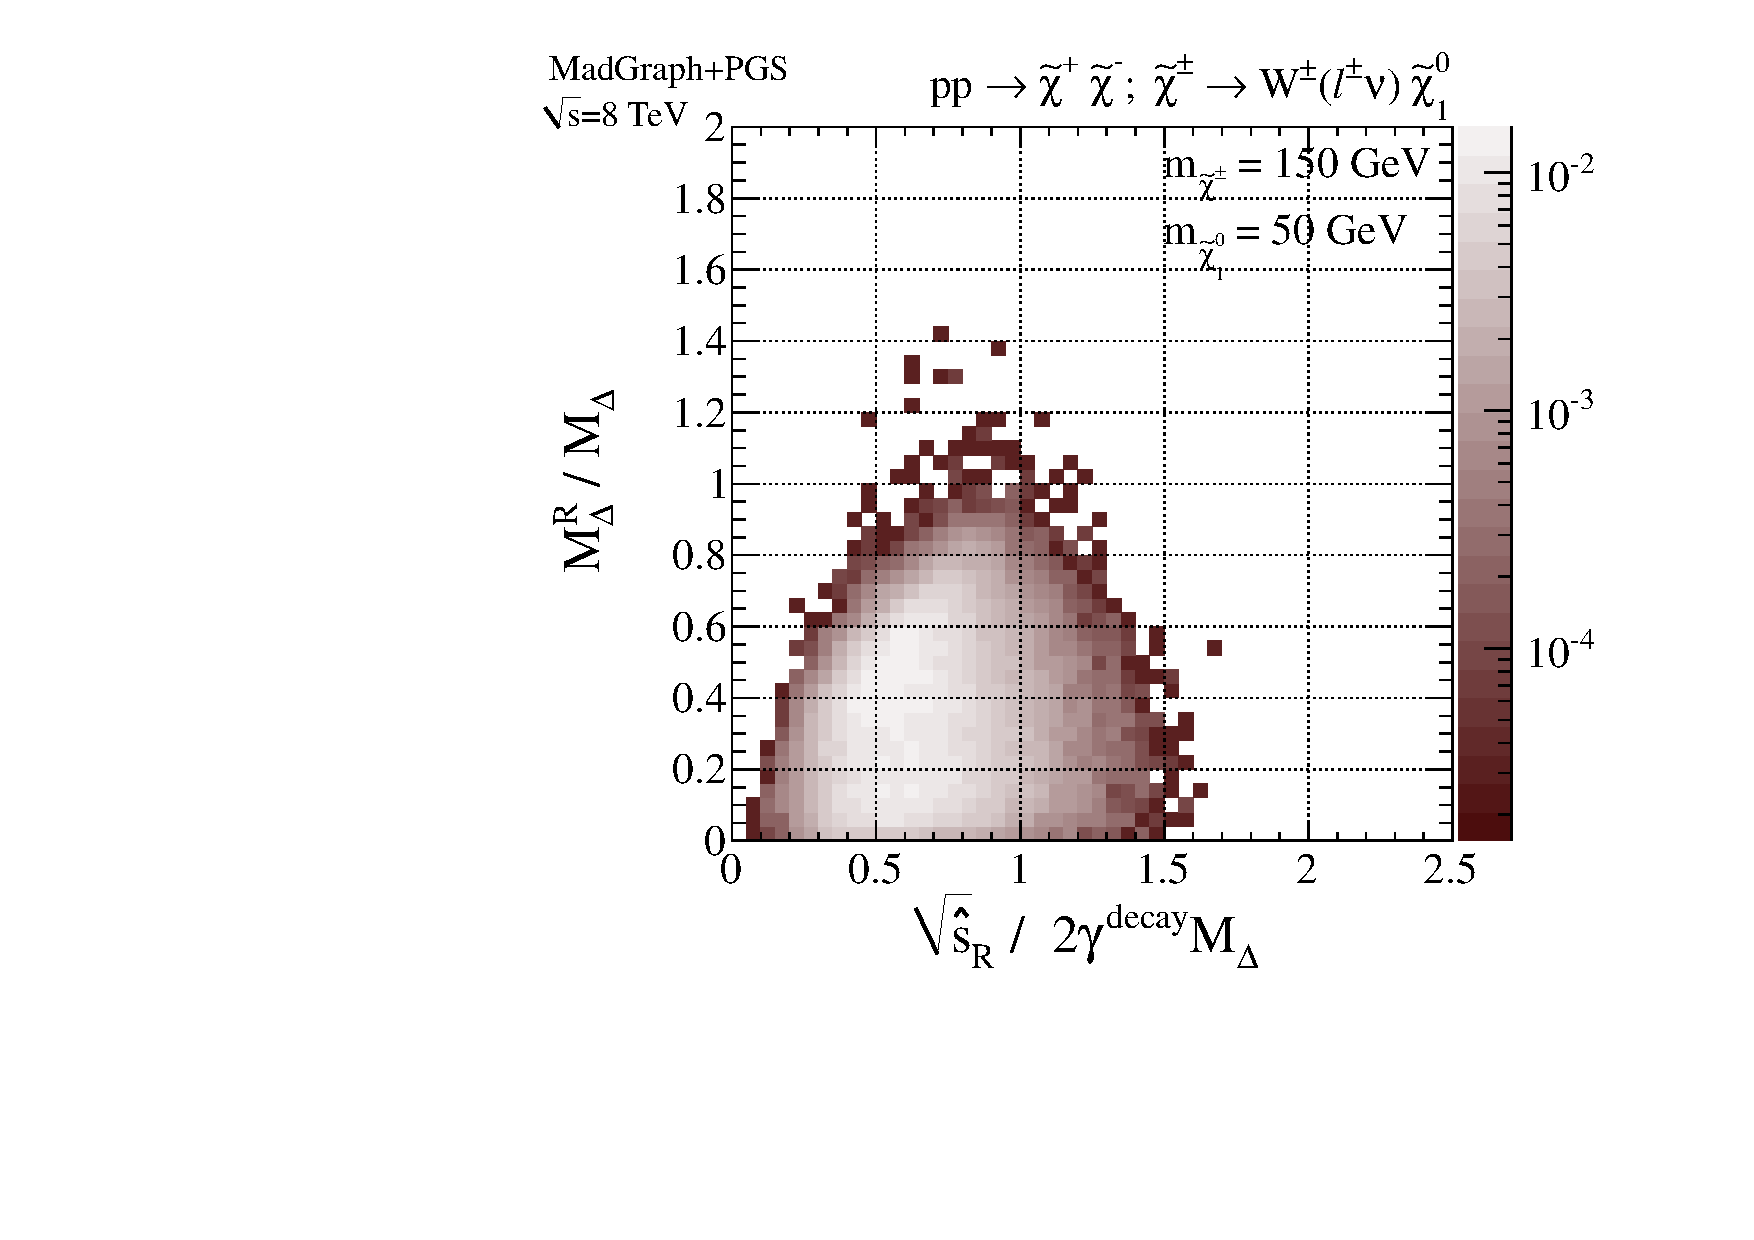
\includegraphics[width=0.32\columnwidth]{fig/sectionII/Mdelta_norm_v_shat_norm_chargino_150_50.pdf}
%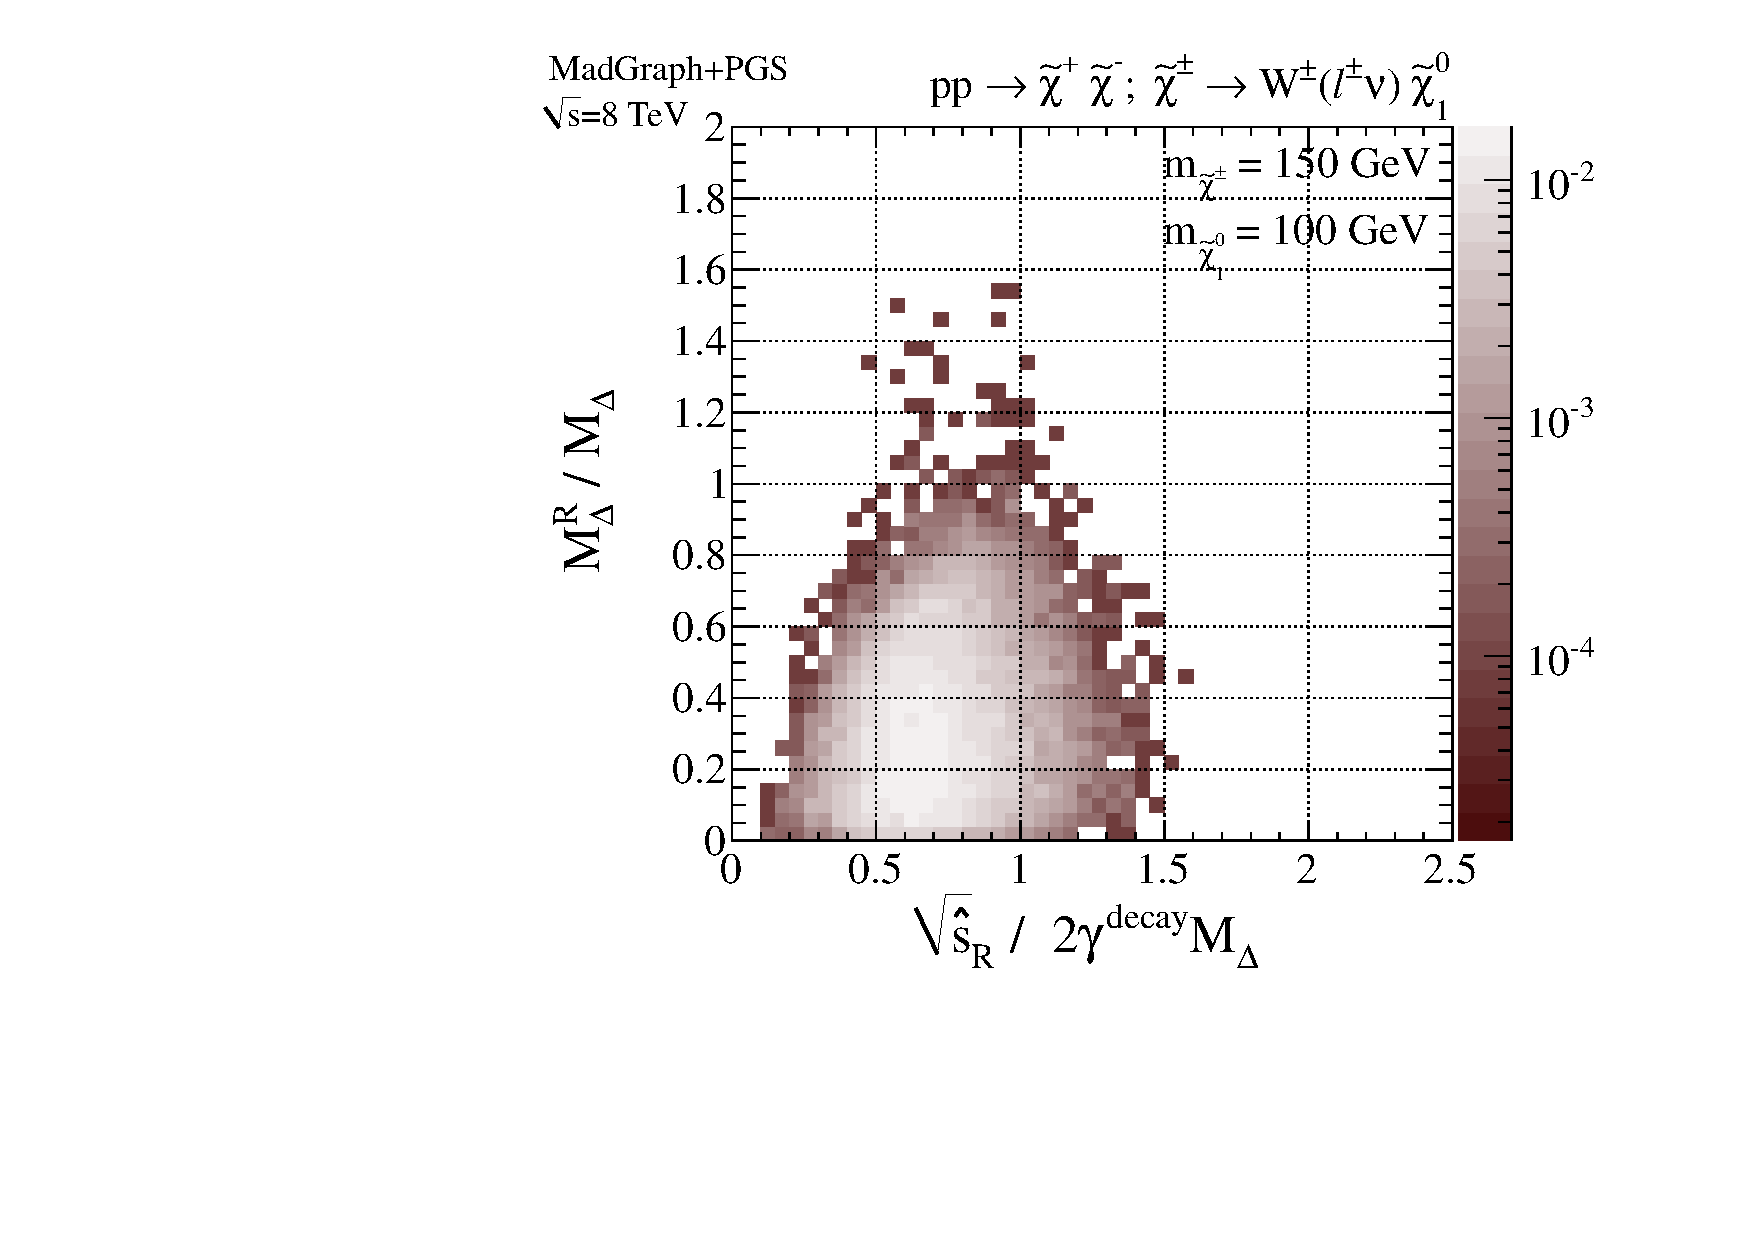
\includegraphics[width=0.32\columnwidth]{fig/sectionII/Mdelta_norm_v_shat_norm_chargino_150_100.pdf}
%\caption{Top Row: Distributions of $\sqrt{\hat{s}}_R$ for a range of $(m_{\tilde{e}}, m_{\tilde{\chi}})$ signal points (left), and distributions of $M_\Delta^R$ (right).  \\
%Bottom row: distributions of $\sqrt{\hat{s}}_R$ normalized to $2 \gamma^{\rm decay} M_\Delta$ (left), and distributions of $M_\Delta^R$ normalized to $M_\Delta$ (right).  \label{fig:compare_razor2}}
%\end{figure}

%\begin{figure}[ht]
%\includegraphics[width=0.4\columnwidth]{fig/sectionII/Mdelta_norm_v_shat_norm_WW.pdf}
%\caption{Top Row: Distributions of $\sqrt{\hat{s}}_R$ for a range of $(m_{\tilde{e}}, m_{\tilde{\chi}})$ signal points (left), and distributions of $M_\Delta^R$ (right).  \\
%Bottom row: distributions of $\sqrt{\hat{s}}_R$ normalized to $2 \gamma^{\rm decay} M_\Delta$ (left), and distributions of $M_\Delta^R$ normalized to $M_\Delta$ (right).  \label{fig:compare_razor2}}
%\end{figure}

Both $\hat{s}_R$ and $M_\Delta^R$ contain information about the mass splitting $M_\Delta$ for signal events. In Figure~\ref{fig:compare_shat_mdelta}, we plot the two variables (normalized to the physical quantities they estimate). Two things can be seen from these plots. First, the variables $\hat{s}_R$ and $M_\Delta^R$ are not degenerate; though both estimate the same quantity ($M_\Delta$), they contain independent kinematic information in that estimation. Secondly, we see that the scatter of the $\hat{s}_R$ around the true value is minimized near the edge structure of the $M_\Delta^R$ variable. This second piece of information will not be fully utilized in our analyses for computational simplicity, though it may provide a useful handle in the future.

As with the original razor variables $M_R$ and $M_T^R$, one or both of these new razor variables could be used. However, we would ideally like a variables that encapsulated information not about $M_\Delta$, but about the overall mass scale of the new particles in the event. This would help distinguish signal from background, especially in the cases where the mass difference is very small ({\it i.e.}~parent and invisible daughter are nearly degenerate in mass), or when the mass difference approaches the mass of the $W$. 

To try to capture more information about the event, we move beyond the mass variables already introduced and look at kinematic angles. In particular, we will be interested in the azimuthal angle between the razor boost $\vec{\beta}_R$ between the lab and $R$ frames and the sum of the visible momenta $\vec{q}_1+\vec{q}_2$, calculated in the razor frame $R$. An illustrative example of the relevant kinematics and angle definition is shown in Figure~\ref{fig:deltaphi}. We call this angle $\Delta \phi_R^{\beta}$, as it is the difference in azimuthal angle between the visible system and the boost $\vec{\beta}_R$, all defined in the razor frame $R$. 

This angle is useful because it inherits information about ratio of masses of the pair produced particles and their invisible daughters, and so can be used in conjunction with a variable such as $M_\Delta^R$ or $\sqrt{\hat{s}}_R$, which have information about the mass difference $M_\Delta$, as previously discussed. The sensitivity of this angular variable to the ratio of masses actually comes from the previously discussed systematic shift of the variable $\sqrt{\hat{s}}_R$ relative to the mass difference $M_\Delta$. As can be seen from Figures~\ref{fig:beta} and \ref{fig:compare_hats}, our estimators of $\beta^{\,\rm CM}$ and $\hat{s}$ ($\beta_R$ and $\hat{s}_R$), do not completely track the center of mass energy of the pair production. $\sqrt{\hat{s}}_R$, for example, is systematically smaller than $\hat{s}$, and $\beta_R$ systematically larger than $\beta^{\, \rm CM}$. This behavior can be easily understood: it is due to the assumption that the energy of the event is evenly split between the visible and invisible systems. For events with invisible particles that are heavy compared to the parent, this assumption will underestimate the energy associated with the missing transverse momentum, and thus $\hat{s}_R$ is an underestimate of $\hat{s}$.

If $\hat{s}_R < \hat{s}$, then the boost $\vec{\beta}_R$ built using $\hat{s}_R$ will be systematically larger than the correct boost $\vec{\beta}^{\, \rm CM}$. In the CM frame, the distribution of the sum of the visible particles relative to the boost direction should be relatively flat. However, if we are ``over-boosting'' from the lab frame to the approximation of the CM frame, then the sum of the visible momenta will tend to be anti-aligned with the boost direction. That is, for systems where $m_\chi/m_S \ll 1$, we expect that the azimuthal angle between $\beta_R$ and $\sum q_i$ will have a peak near $\Delta\phi_R^{\beta} \sim \pi$. In Figure~\ref{fig:deltaRbeta}, we show the distribution of this angle for a range of neutralino masses (for a fixed slepton or chargino mass). As can be seen, as the ratio $m_\chi/m_S$ approaches one, the peak of the distribution near $\pi$ becomes more pronounced. Note the large drop in statistics for chargino events where the mass of the neutralino approaches that of the parent chargino. With such a mass spectrum, events have difficulty passing the selection criteria, which will be discussed in more detail in the next section. 

Notice also from this figure that sleptons decaying to massless neutralinos are very similar to the $W^+W^- \to \ell^-\ell^+ \nu\nu$ background. This is as expected, as the $WW$ background is a case where the invisible particles (neutrinos) are massless, and so our estimate of $\hat{s}_R$ for this background will overboost to the $R$ frame, just as with the massless signal case. Thus, we do not expect this angle to be of great use in the massless neutralino limit, however, it will be of significant help in distinguishing from background in the near-degenerate limit, where traditional mass variables sensitive to $M_\Delta$ are less effective. We also comment that the Drell-Yan $Z \to \ell \ell$ background, also shown in Figure~\ref{fig:deltaRbeta}, has a strong peak near $\Delta\phi_R^{\beta}\sim 0$. In this case, we are underboosting compared to the correct CM frame, as we are assuming that there is real missing transverse energy in an event that has no invisible particles.

In the $R$-frame, there is one final kinematic variable that we can construct. The variable $\sqrt{\hat{s}}_R$ is our estimate of the total energy available in the pair-production event. In the razor frame $R$, it can be divided up into three components:
\begin{equation}
\frac{\hat{s}_R}{4} = (M_\Delta^R)^2+(q_{1R}+q_{2R})^2+(E_{1R}-E_{2R})^2. \label{eq:shatRexpansion}
\end{equation}
$M_\Delta^R$ and the invariant mass of the visible system $\sqrt{(q_{1R}+q_{2R})^2}$ have already been considered. However, the energy difference of the visible particles, $E_{1R}-E_{2R}$, has not been used. As with $\hat{s}_R$ and $M_\Delta^R$, the overall mass scale of $E_{1R}-E_{2R}$ is sensitive to $M_\Delta$, and is thus degenerate with our other mass variables. We therefore construct a new dimensionless variable
\begin{equation}
|\cos\theta_{R+1}|^2 = \frac{(E_{1R}-E_{2R})^2}{\hat{s}_R/4-(M_\Delta^R)^2} = \frac{\hat{s}_R/4-(M_\Delta^R)^2-(q_{1R}+q_{2R})^2}{\hat{s}_R/4-(M_\Delta^R)^2}. \label{eq:costhetaR1}
\end{equation}
This particular definition (and identification as a cosine of an angle) is because this variable can also be interpreted as the angle between the boost direction $\vec{\beta}_R$ and the direction of $q_1$ or $q_2$ in the frame $R+1$. However, it is more useful to think of this angle as a measure of the energy difference between the two visible particles.

A measure of the energy difference is useful in background rejection, especially in removing $W^-W^+$ events. The reasoning is as follows: for scalar particles, the decay of the parent into the visible and invisible daughters has a flat angular distribution in the parent's rest frame. In the production frame, we do not then expect a large correlation between the energy of the two visible particles. Though in their respective decay frames each has the same energy, the orientation of their momentum relative to the momentum of the parent is uncorrelated, and so $|E_1 - E_2| \propto |\cos\theta_{R+1}|$ will not cluster at zero. The exception is for very large boosts of the parent particle; in this case, the direction of the visible daughter in the decay frame is effective erased by the very large boost. In such cases, both visible particles are colinear with their parent direction and have $E_1 \approx E_2$.

Now consider $W^-W^+$ background. Unlike scalar decay, the vector $W$ boson decaying into fermions has a correlation in the direction of the visible lepton relative to the parent polarization. As the polarizations of the two $W$ bosons in an event are themselves correlated, this means that, after the boost from the decay frames to the production frame (or to our approximation of that frame, the $R$ frame), the two visible leptons will tend to have similar energies: $E_1 \approx E_2$. Therefore, the distribution of $|\cos\theta_{R+1}|$ for this background will be more highly peaked towards zero. The behavior of signal and background in this variable is shown in Figure~\ref{fig:costheta}, for representative signal points.


In Figure~\ref{fig:costheta_v_MdeltaR}, we show the distributions of $|\cos\theta_{R+1}|$ with respect to $M_\Delta^R$ for a representative choice of slepton and neutralino masses, and compare with the distribution for the $W^-W^+$ background. As can be seen, when $M_\Delta^R \sim 0$, the signal events cluster near $|\cos\theta_{R+1}| = 0$. This makes sense, as $M_\Delta^R \sim 0$ corresponds to large boosts of the parent particles (as can be seen in Eq.~\eqref{eq:mdeltaR}). As $M_\Delta^R$ approaches $M_\Delta$, we recover the essentially flat distribution of $|\cos\theta_{R+1}|$ we expect from a scalar decay. The $W^-W^+$ background, on the other hand, does not have a flat distribution for $M_\Delta^R \sim m_W$. This, therefore, allows for discrimination of signal and background events even for signal events where $M_\Delta \sim m_W$.

These new angular variables demonstrates the utility of the razor boosts. The mass variables ($\hat{s}_R$ and $M_\Delta^R$) are not completely unique to our work; they have been independently developed in different contexts in the past (see Ref.~\cite{Rainwater:1999sd}). However, by associating these variables with a particular set of boosts, we can approximate the CM of the event. This allows us to build additional variables using this approximation, two of which ($\Delta \phi_R^{\beta}$ and $|\cos\theta_{R+1}|$) turn out to encode further information about the event. Furthermore, as the construction of the $|\cos\theta_{R+1}|$ variable relies on the spin of the new particles being searched for, it has the potential to be used as a measurement of spin if new physics is found. This possibility will be investigated in a future work. 

In this study, we work primarily with the set of four variables $\hat{s}_R$, $M_\Delta^R$, $\Delta \phi_R^{\beta}$, and $|\cos\theta_{R+1}|$. The two mass variables are somewhat degenerate, as both are estimators of the mass splitting between the parent and daughter particles. Though there may be some utility in using all four variables in a single analysis, here we will demonstrate the possible reach of our super-razor search by restricting ourselves to the $M_\Delta^R$, $\Delta \phi_R^{\beta}$, and $|\cos\theta_{R+1}|$ combination only. We will also use $\gamma_{R}$ and $\gamma_{R+1}$ in our improved selection criteria to reduce background contamination  We choose $M_\Delta^R$ over $\hat{s}_R$ for our analysis because, as Figure~\ref{fig:deltaphiMdelta} shows, the variables $M_\Delta^R$ and $|\cos\theta_{R+1}|$ are approximately uncorrelated with $\Delta\phi_R^\beta$ for signal events. This simplifies the shape analysis we will discuss in the next section, as it allows us to decompose a 3D analysis into a 2D $\times$ 1D one.

\begin{figure}[ht]
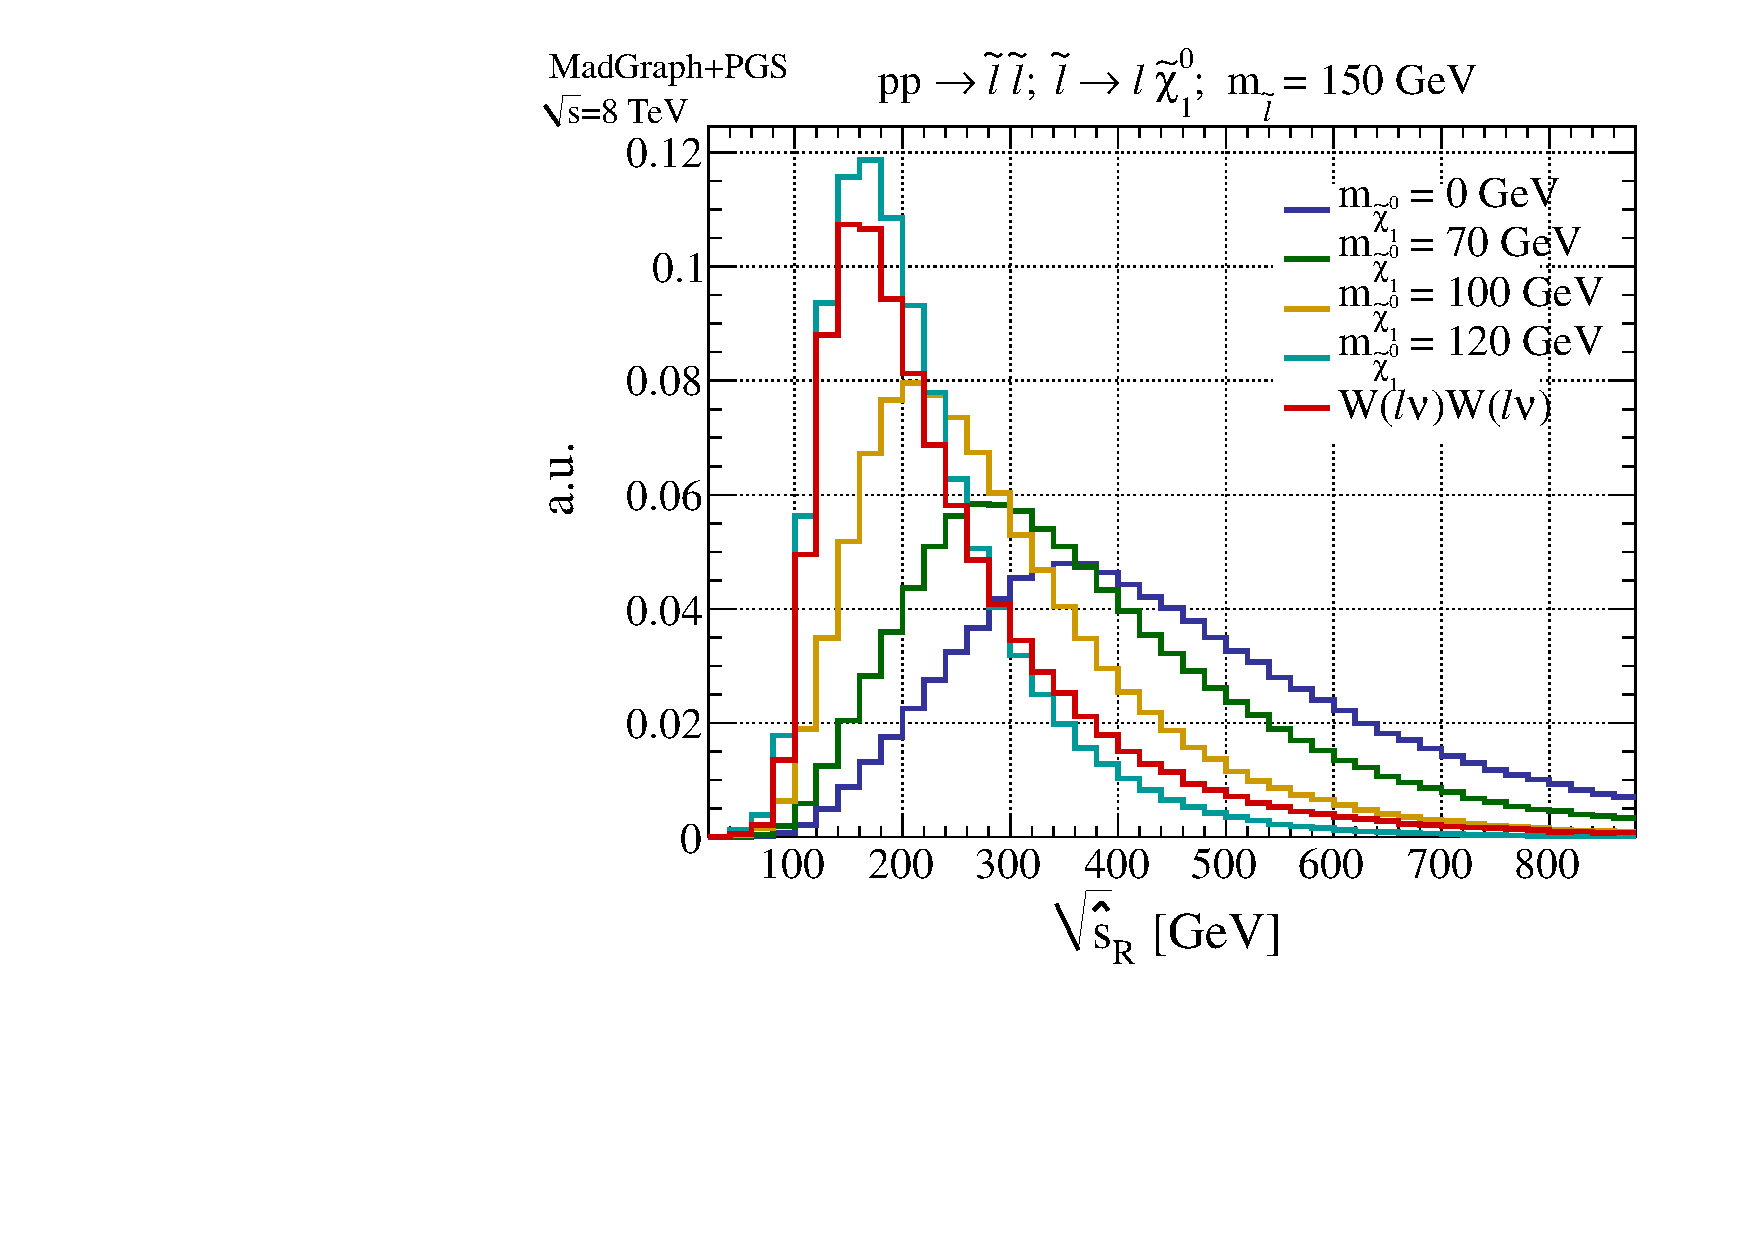
\includegraphics[width=0.35\columnwidth]{fig/sectionII/shat_1D_slepton.pdf}
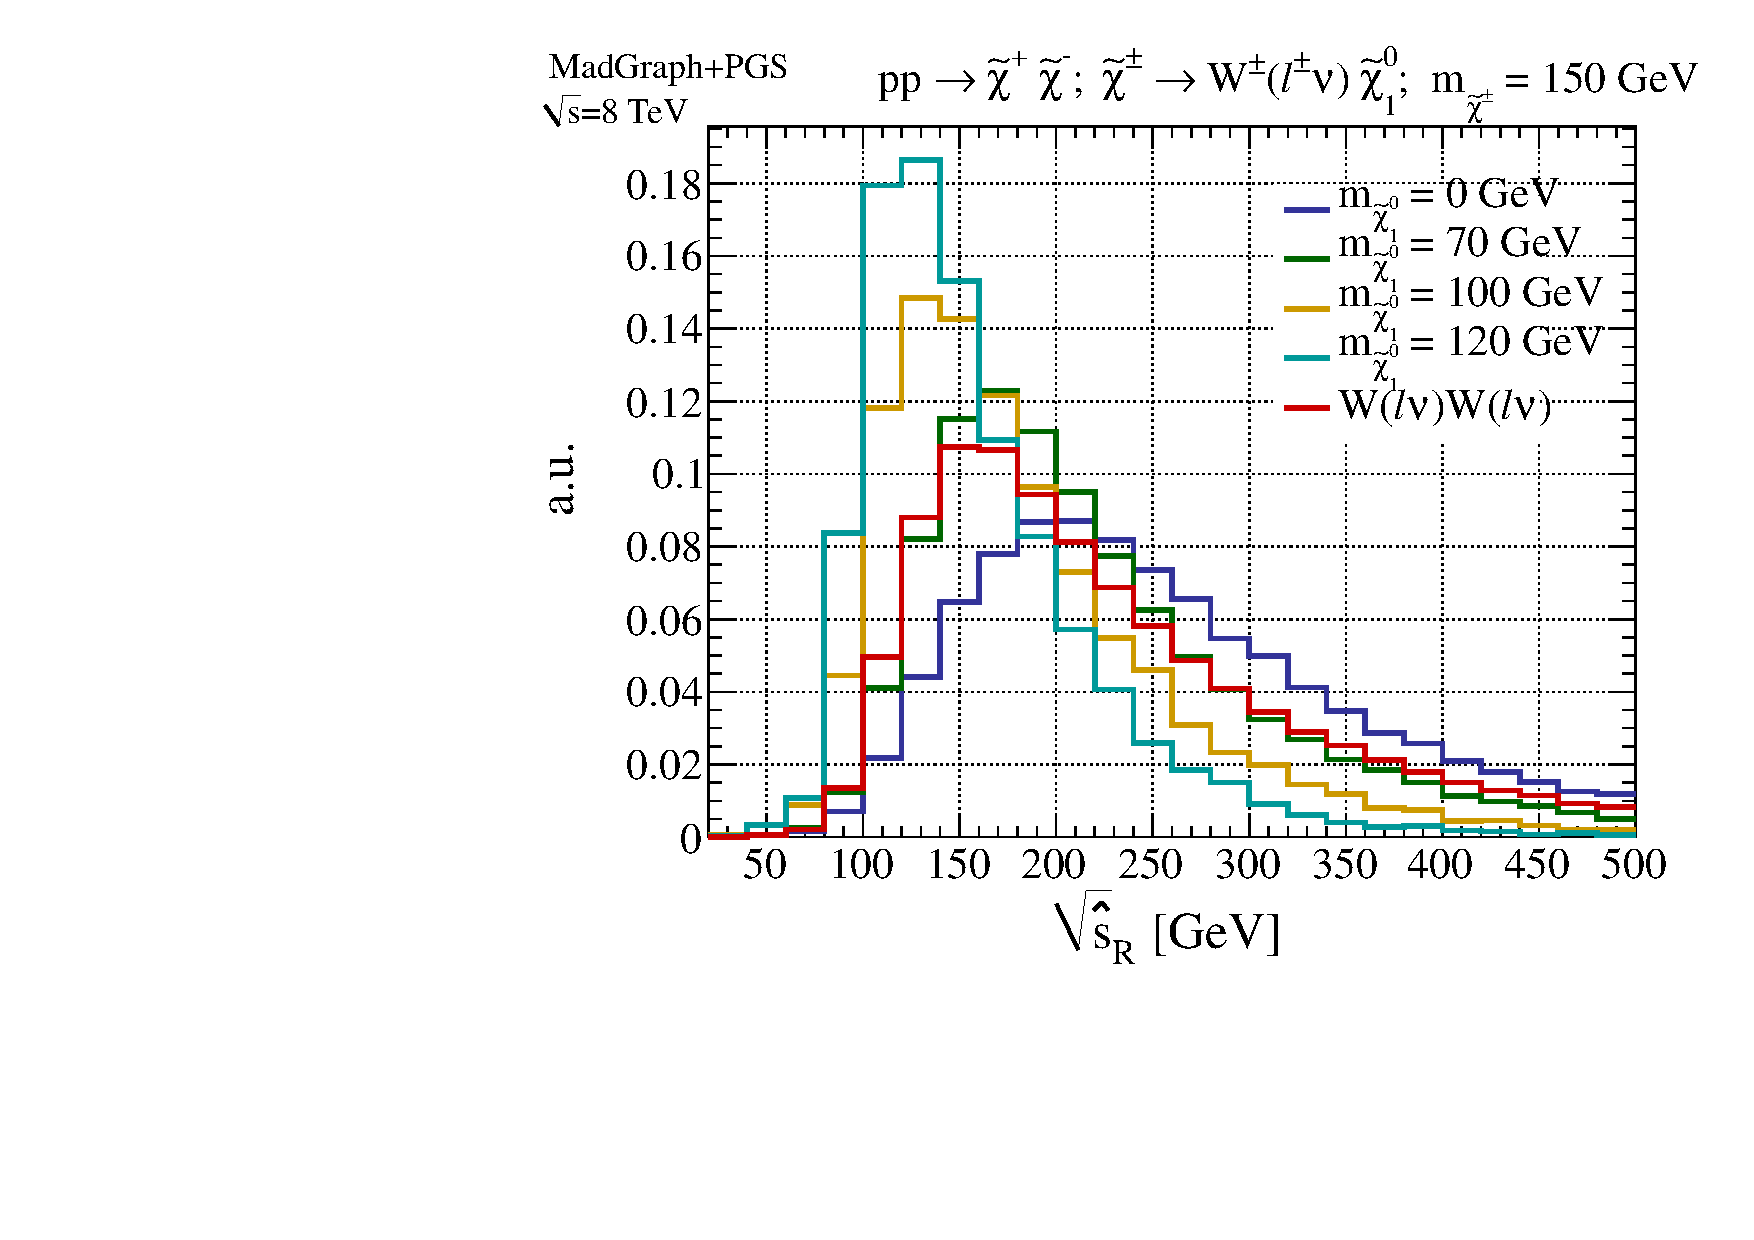
\includegraphics[width=0.35\columnwidth]{fig/sectionII/shat_1D_chargino.pdf}
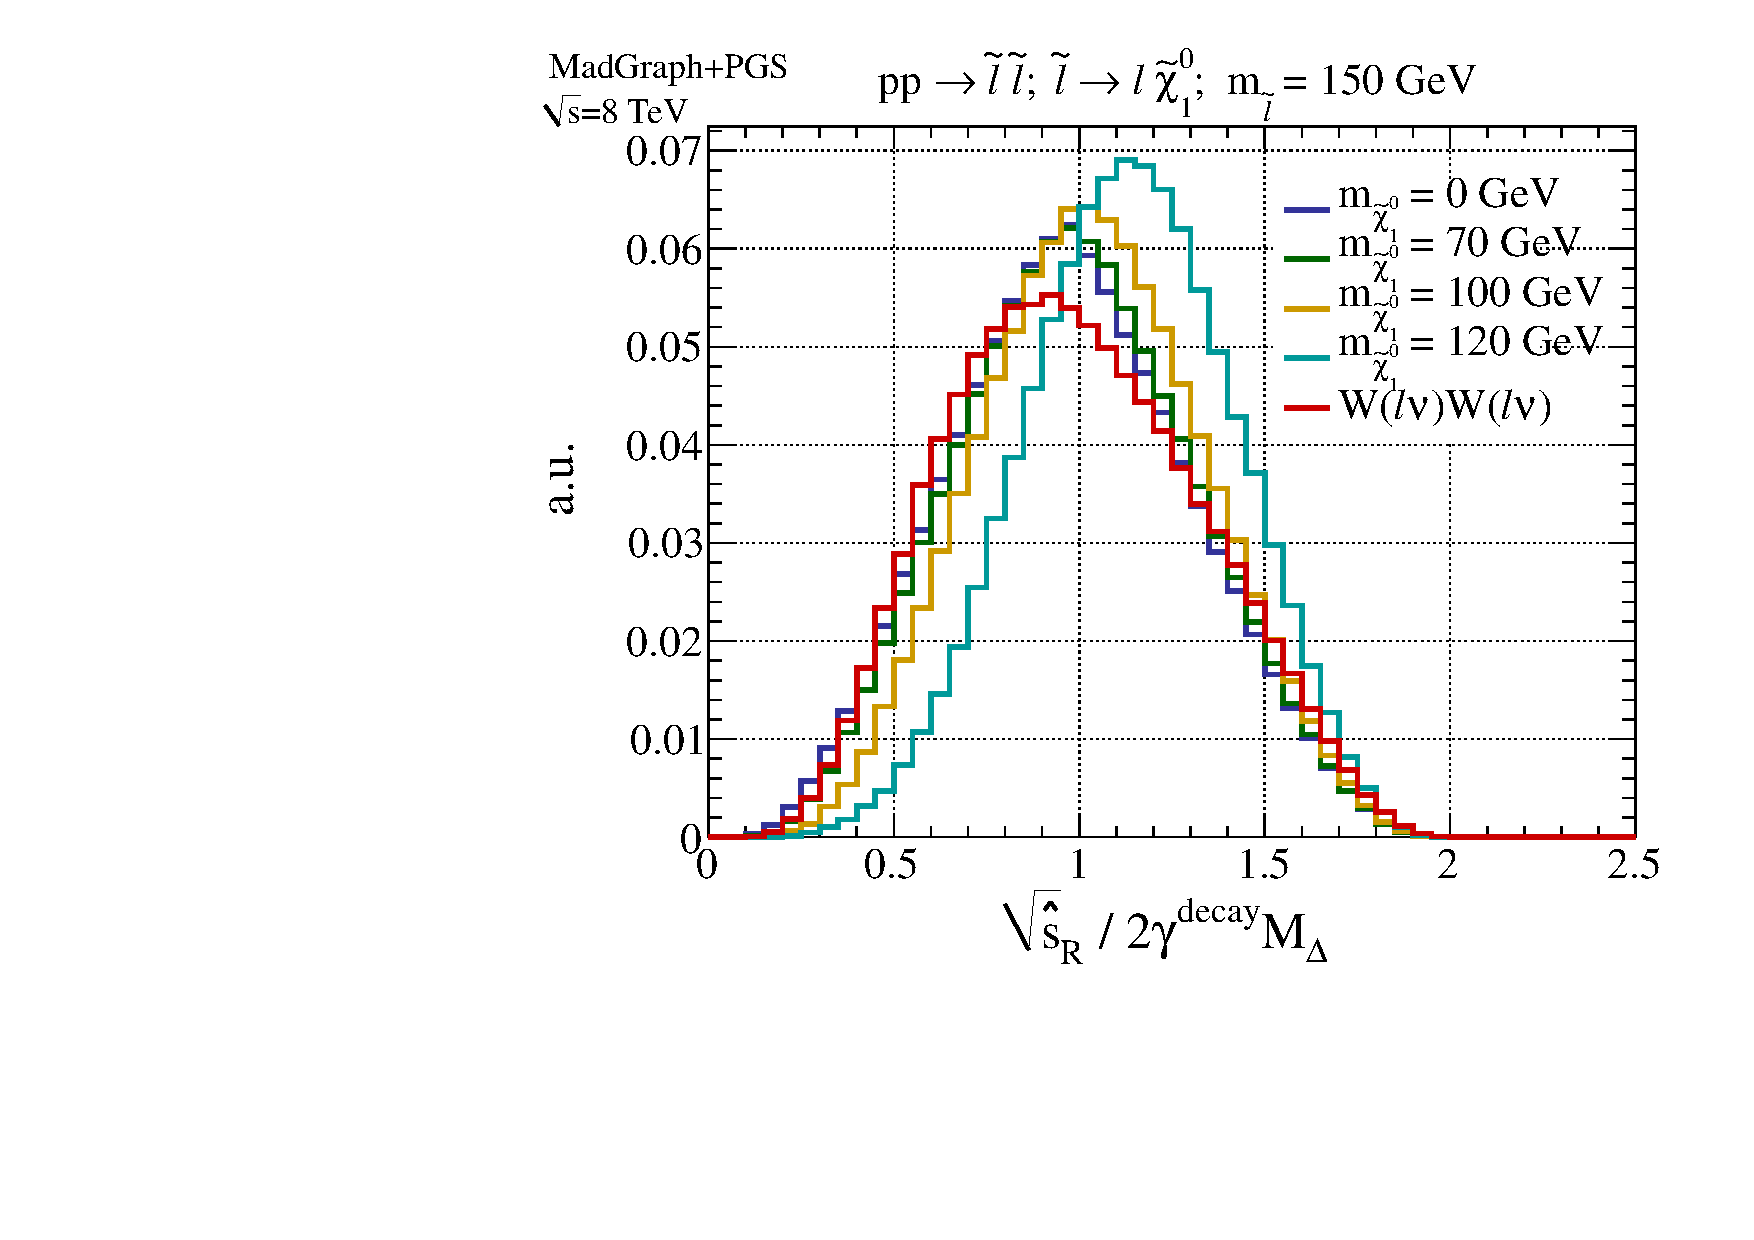
\includegraphics[width=0.35\columnwidth]{fig/sectionII/shat_norm_1D_slepton.pdf}
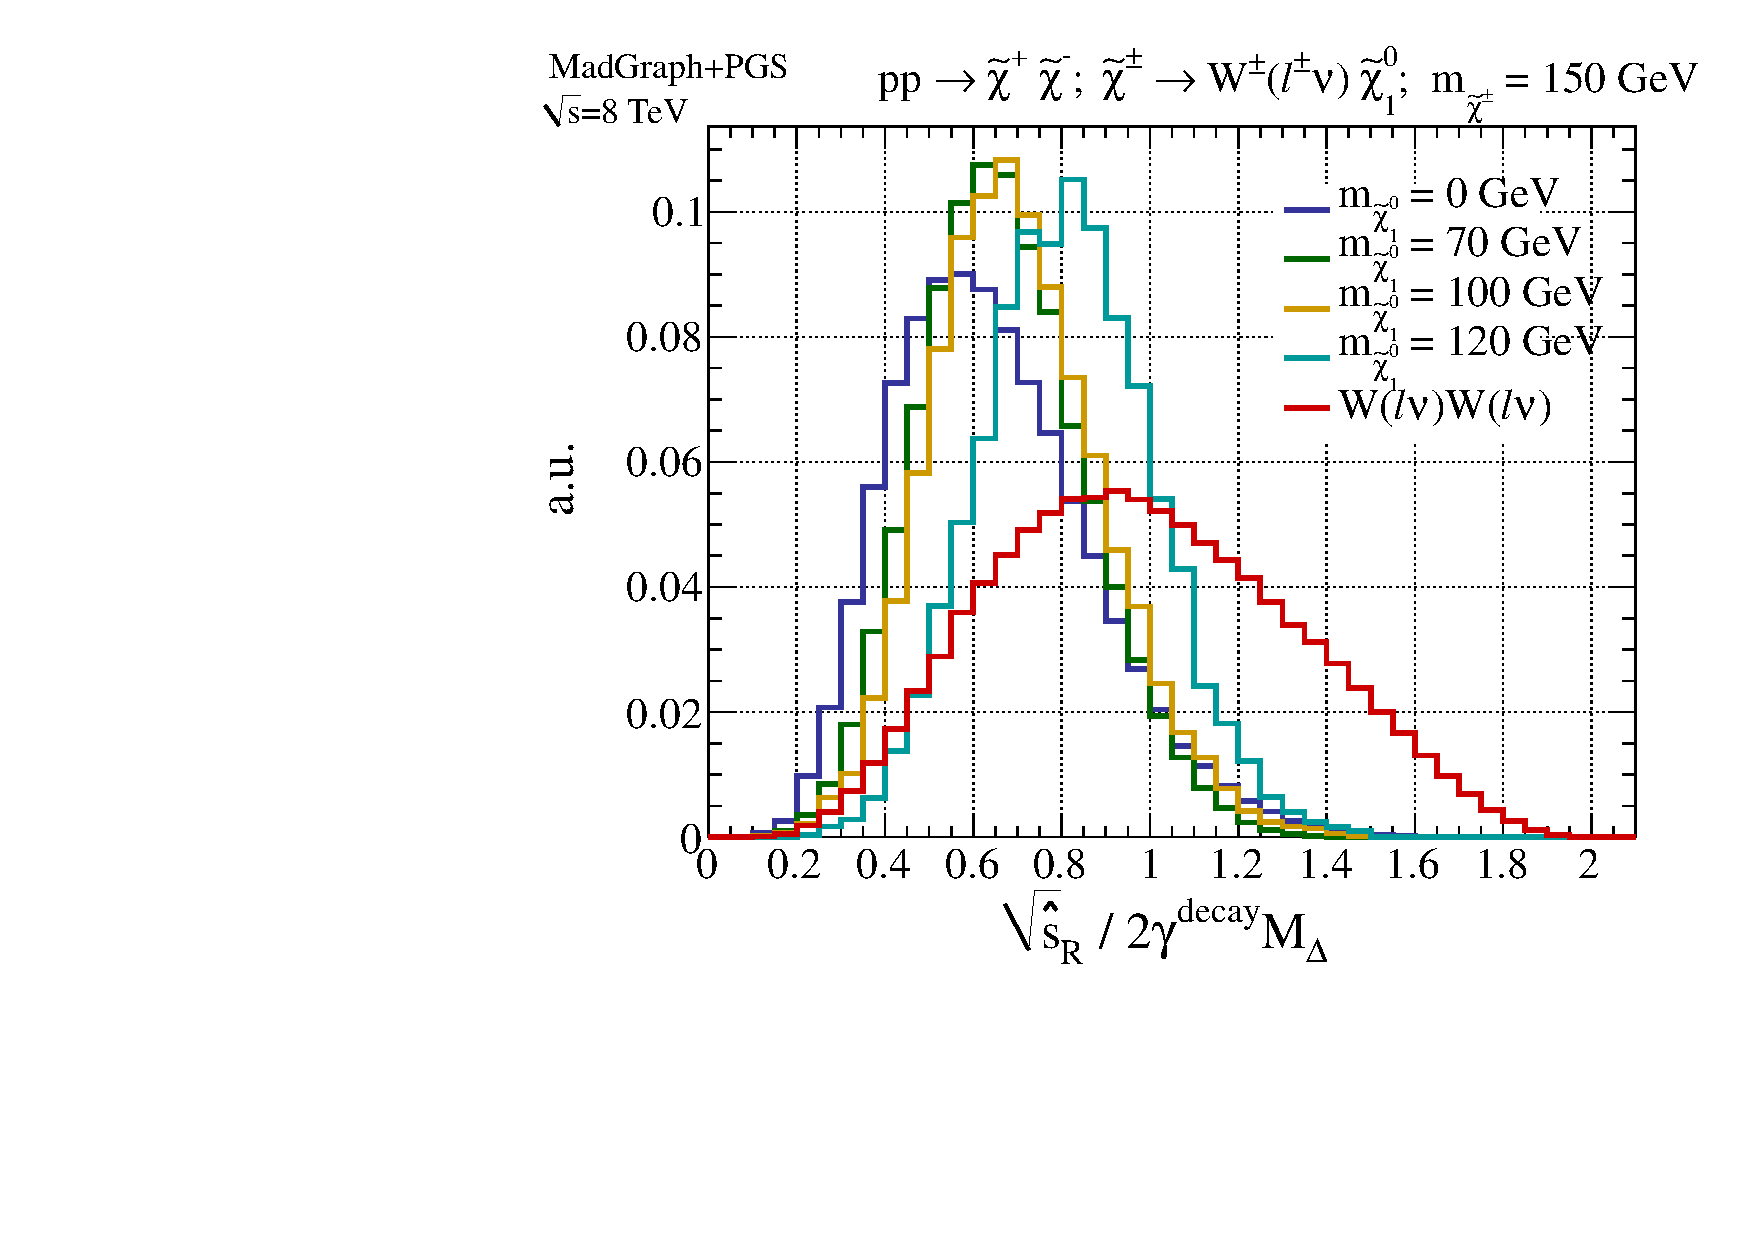
\includegraphics[width=0.35\columnwidth]{fig/sectionII/shat_norm_1D_chargino.pdf}
\caption{Top Row: Distributions of $\sqrt{\hat{s}}_R$ for a 150~GeV slepton (left) or chargino (right) and a range of neutralino masses. Also shown is the distribution of the $W^-W^+$ background.  Bottom row: Distributions of $\sqrt{\hat{s}}_R$ normalized to $2 \gamma^{\rm decay} M_\Delta$ for selectrons (left) and charginos (right), again for a range of neutralino masses. \label{fig:compare_hats}}
\end{figure}

\begin{figure}[ht]
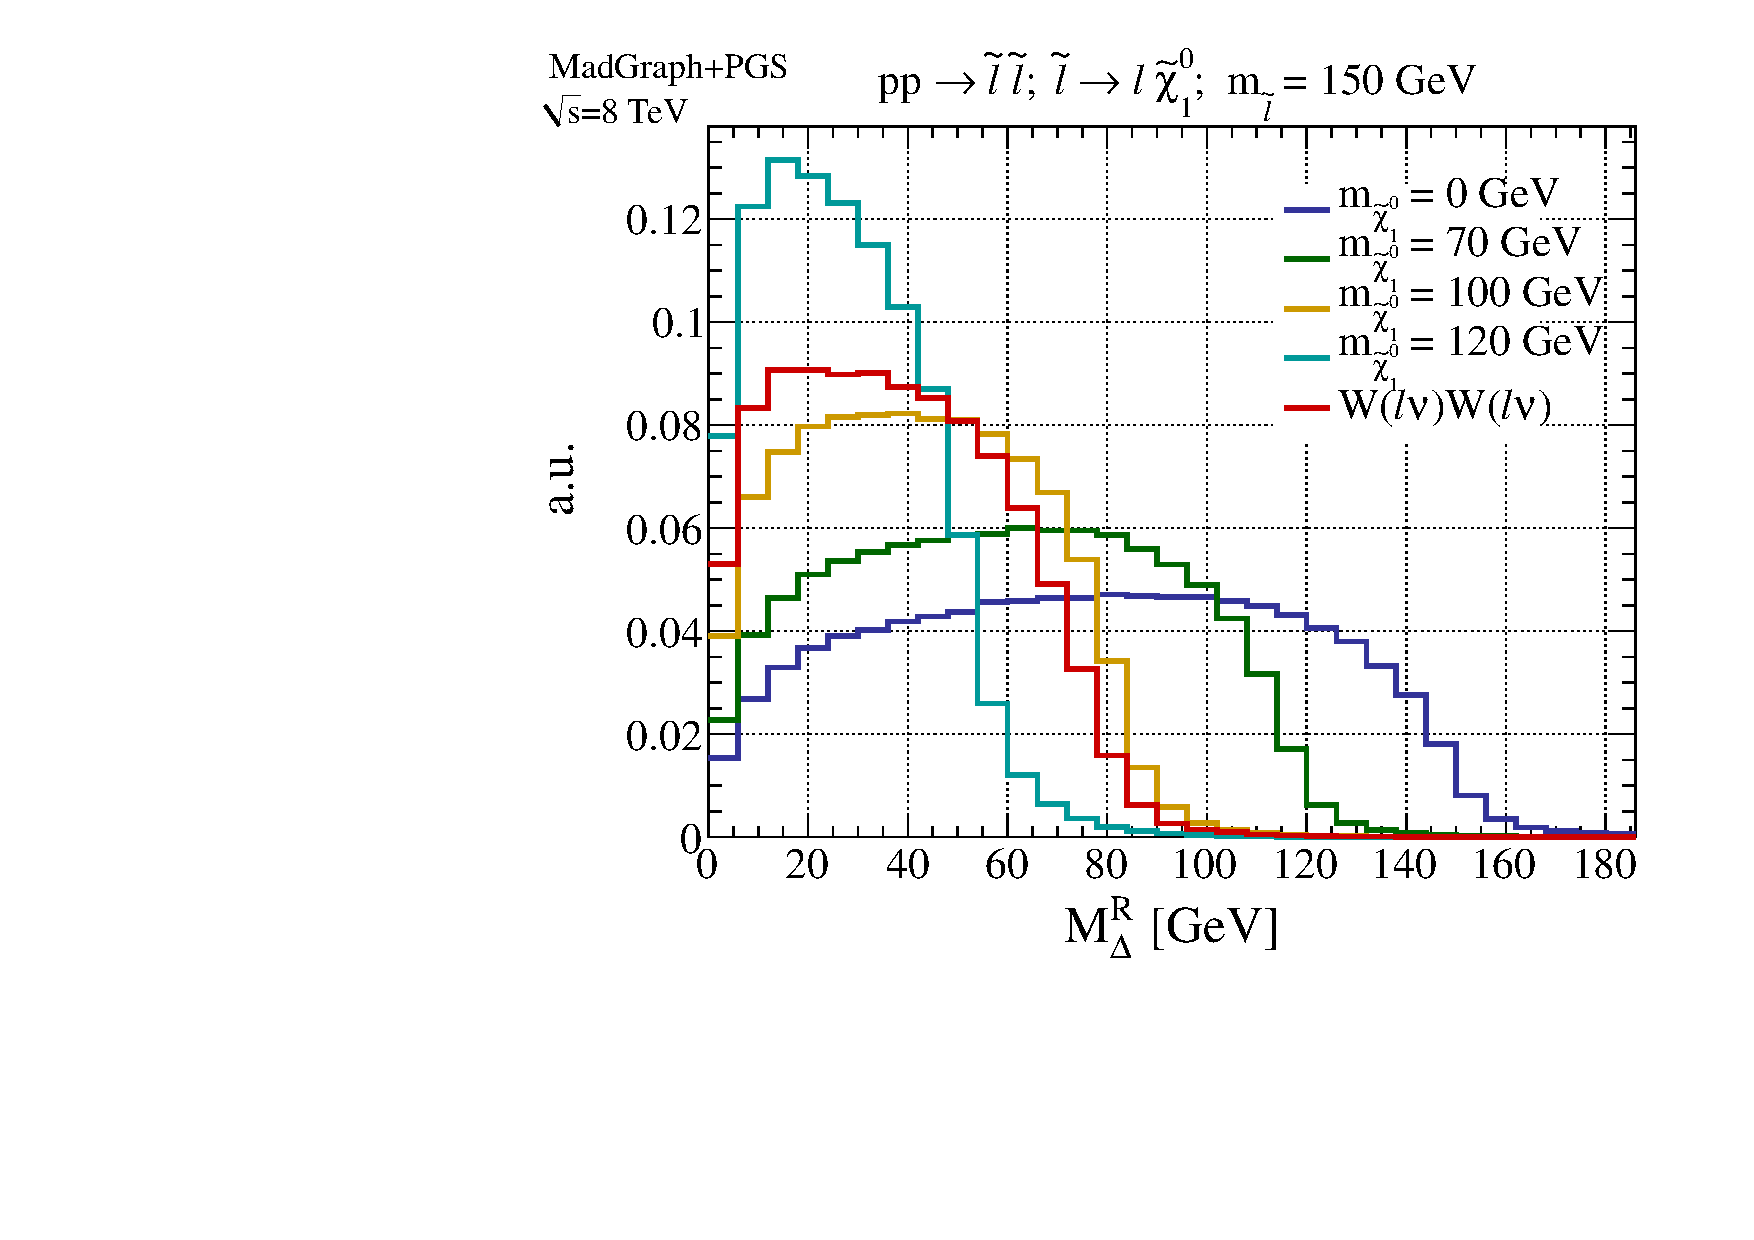
\includegraphics[width=0.35\columnwidth]{fig/sectionII/Mdelta_1D_slepton.pdf}
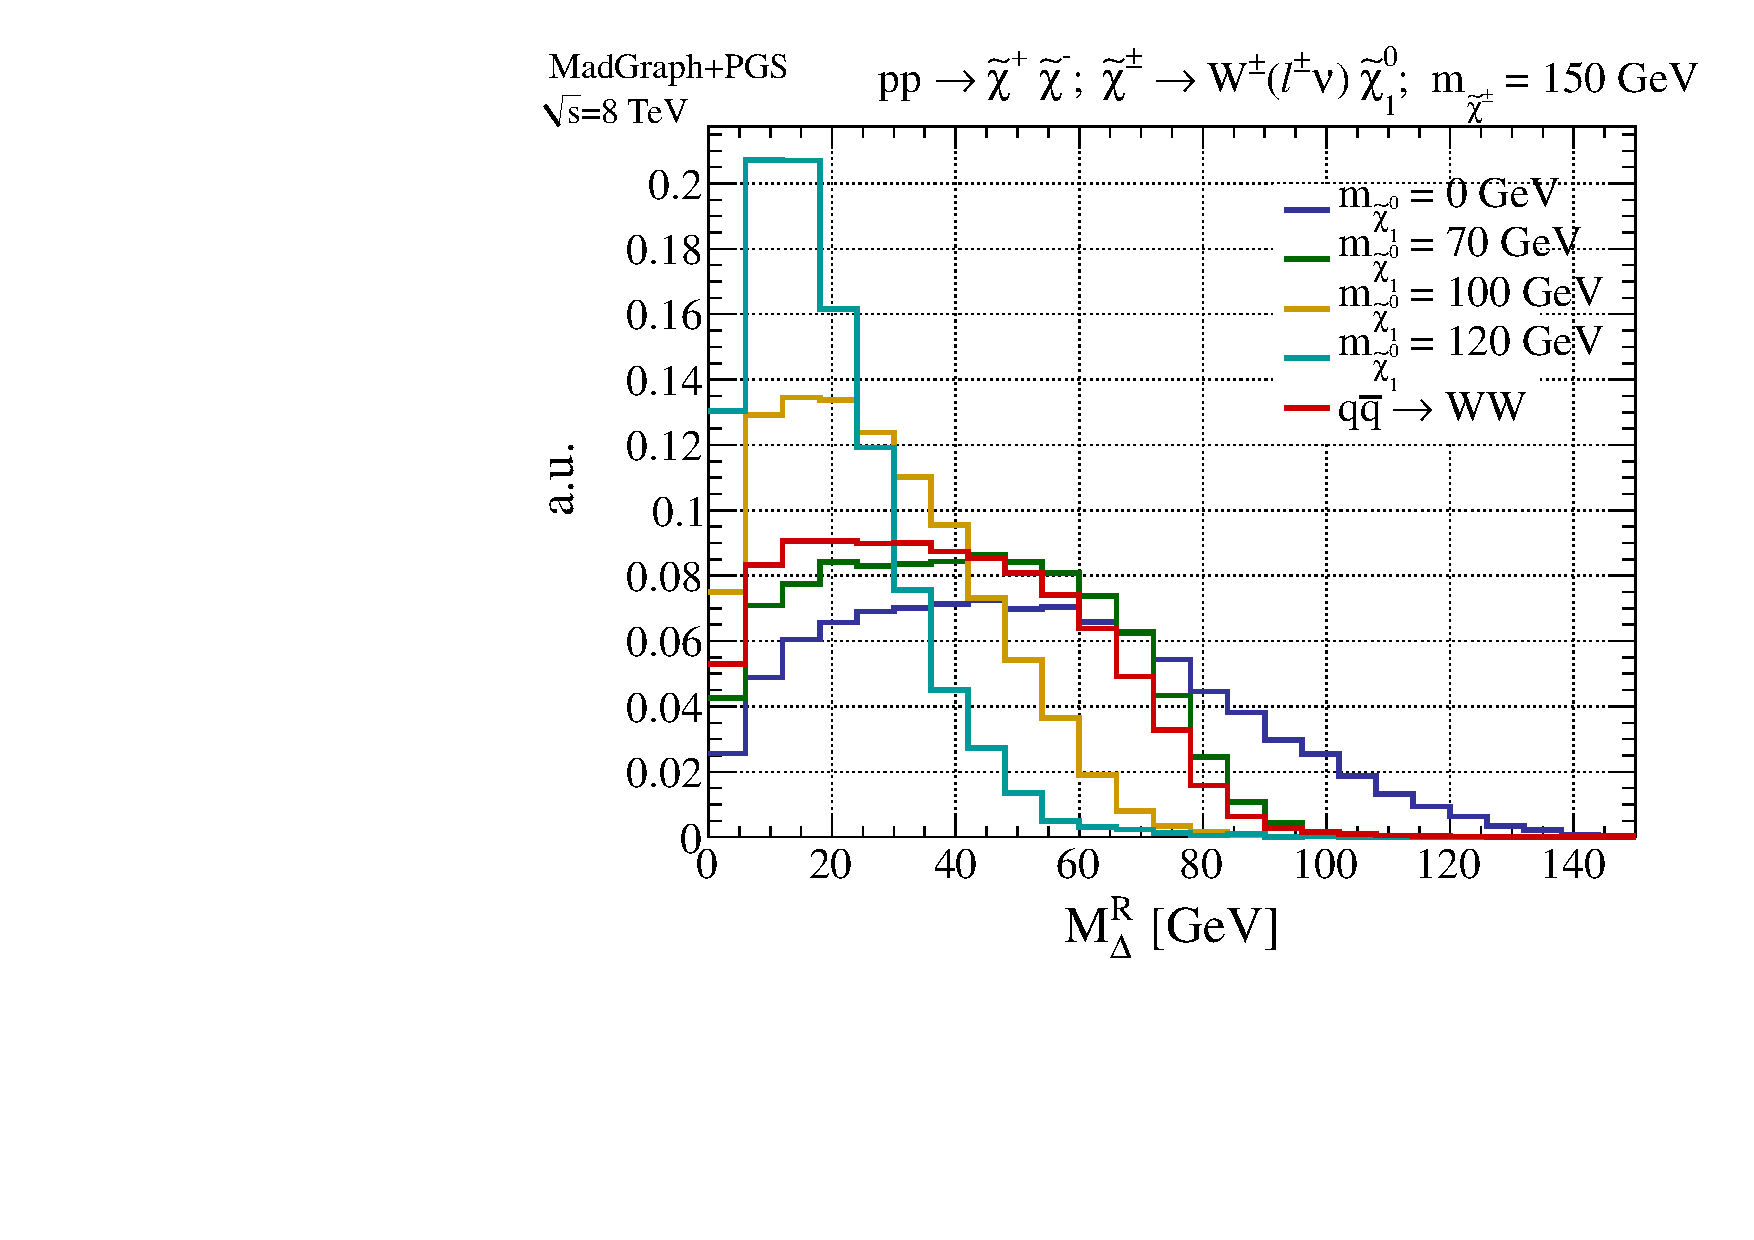
\includegraphics[width=0.35\columnwidth]{fig/sectionII/Mdelta_1D_chargino.pdf}
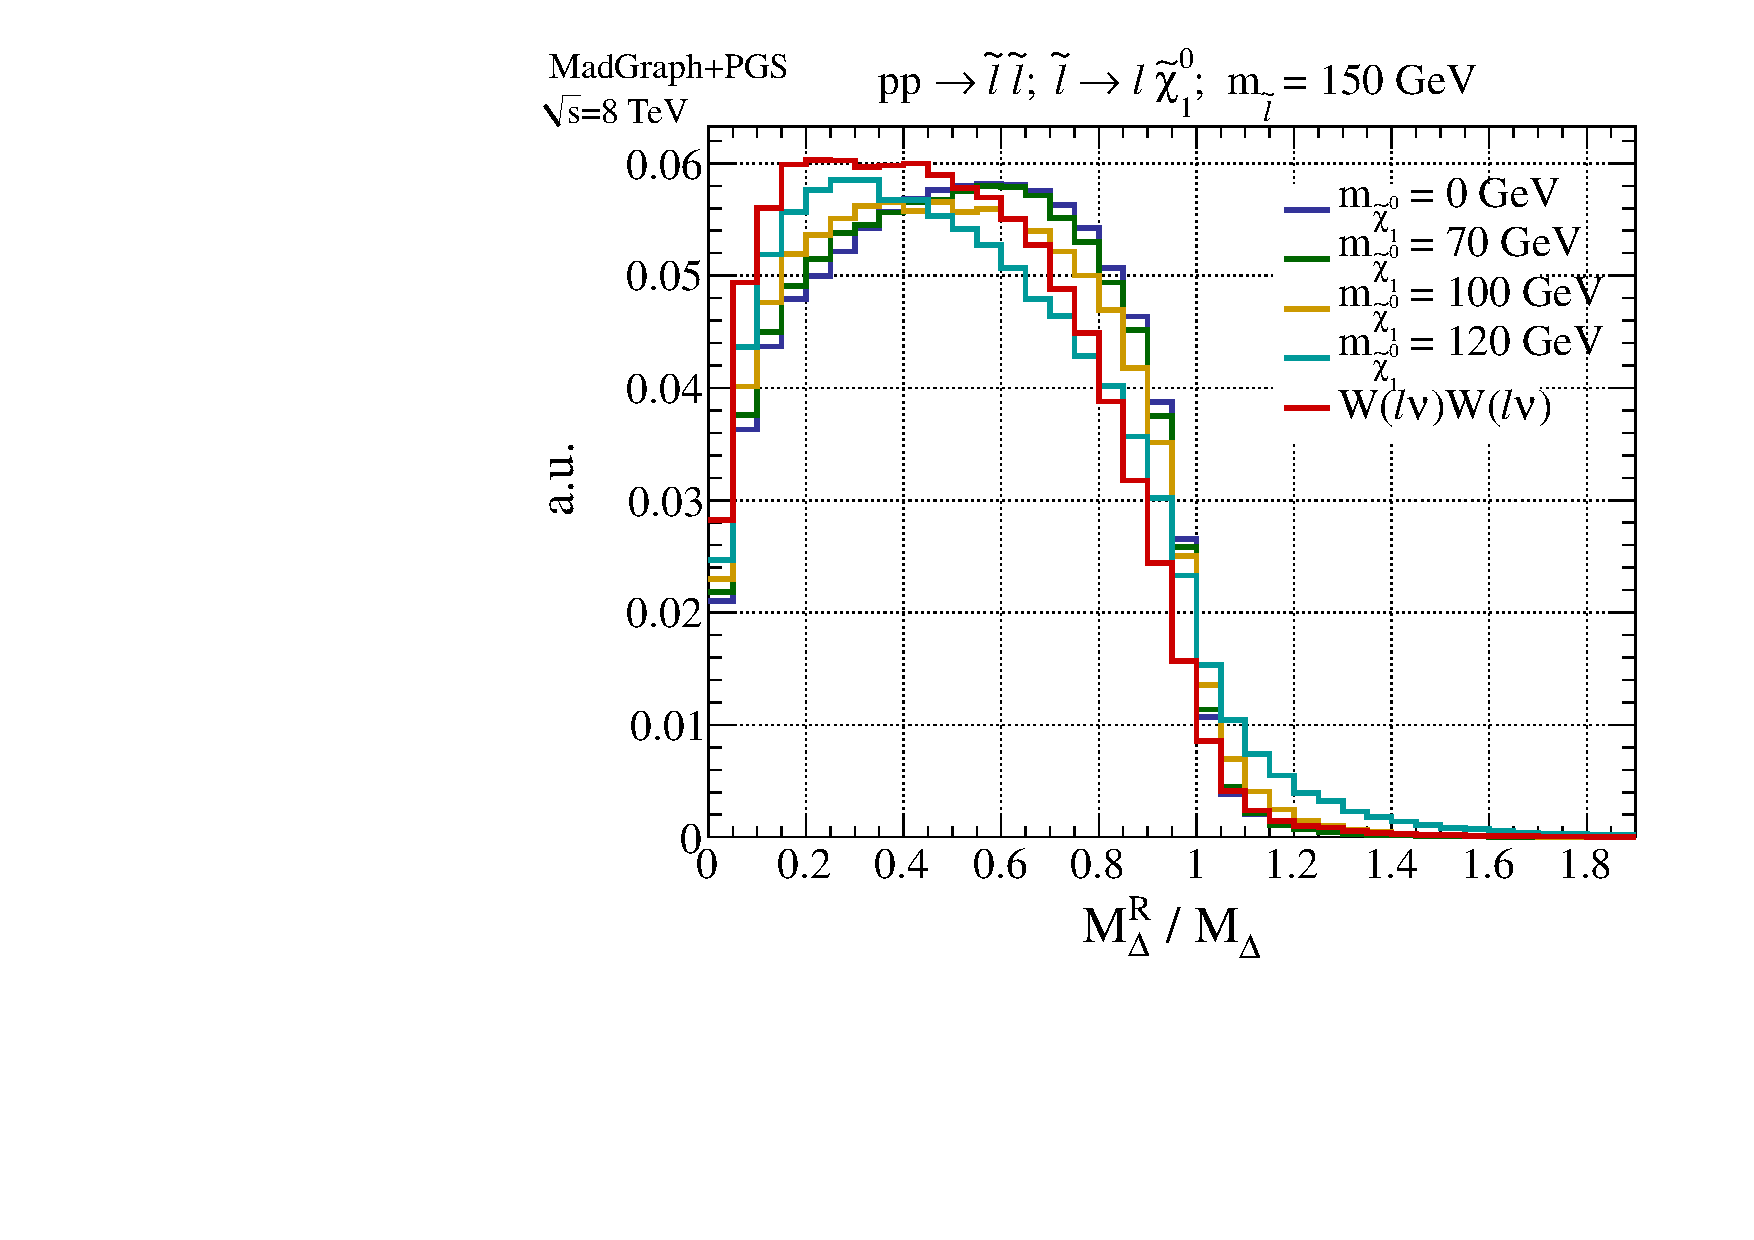
\includegraphics[width=0.35\columnwidth]{fig/sectionII/Mdelta_norm_1D_slepton.pdf}
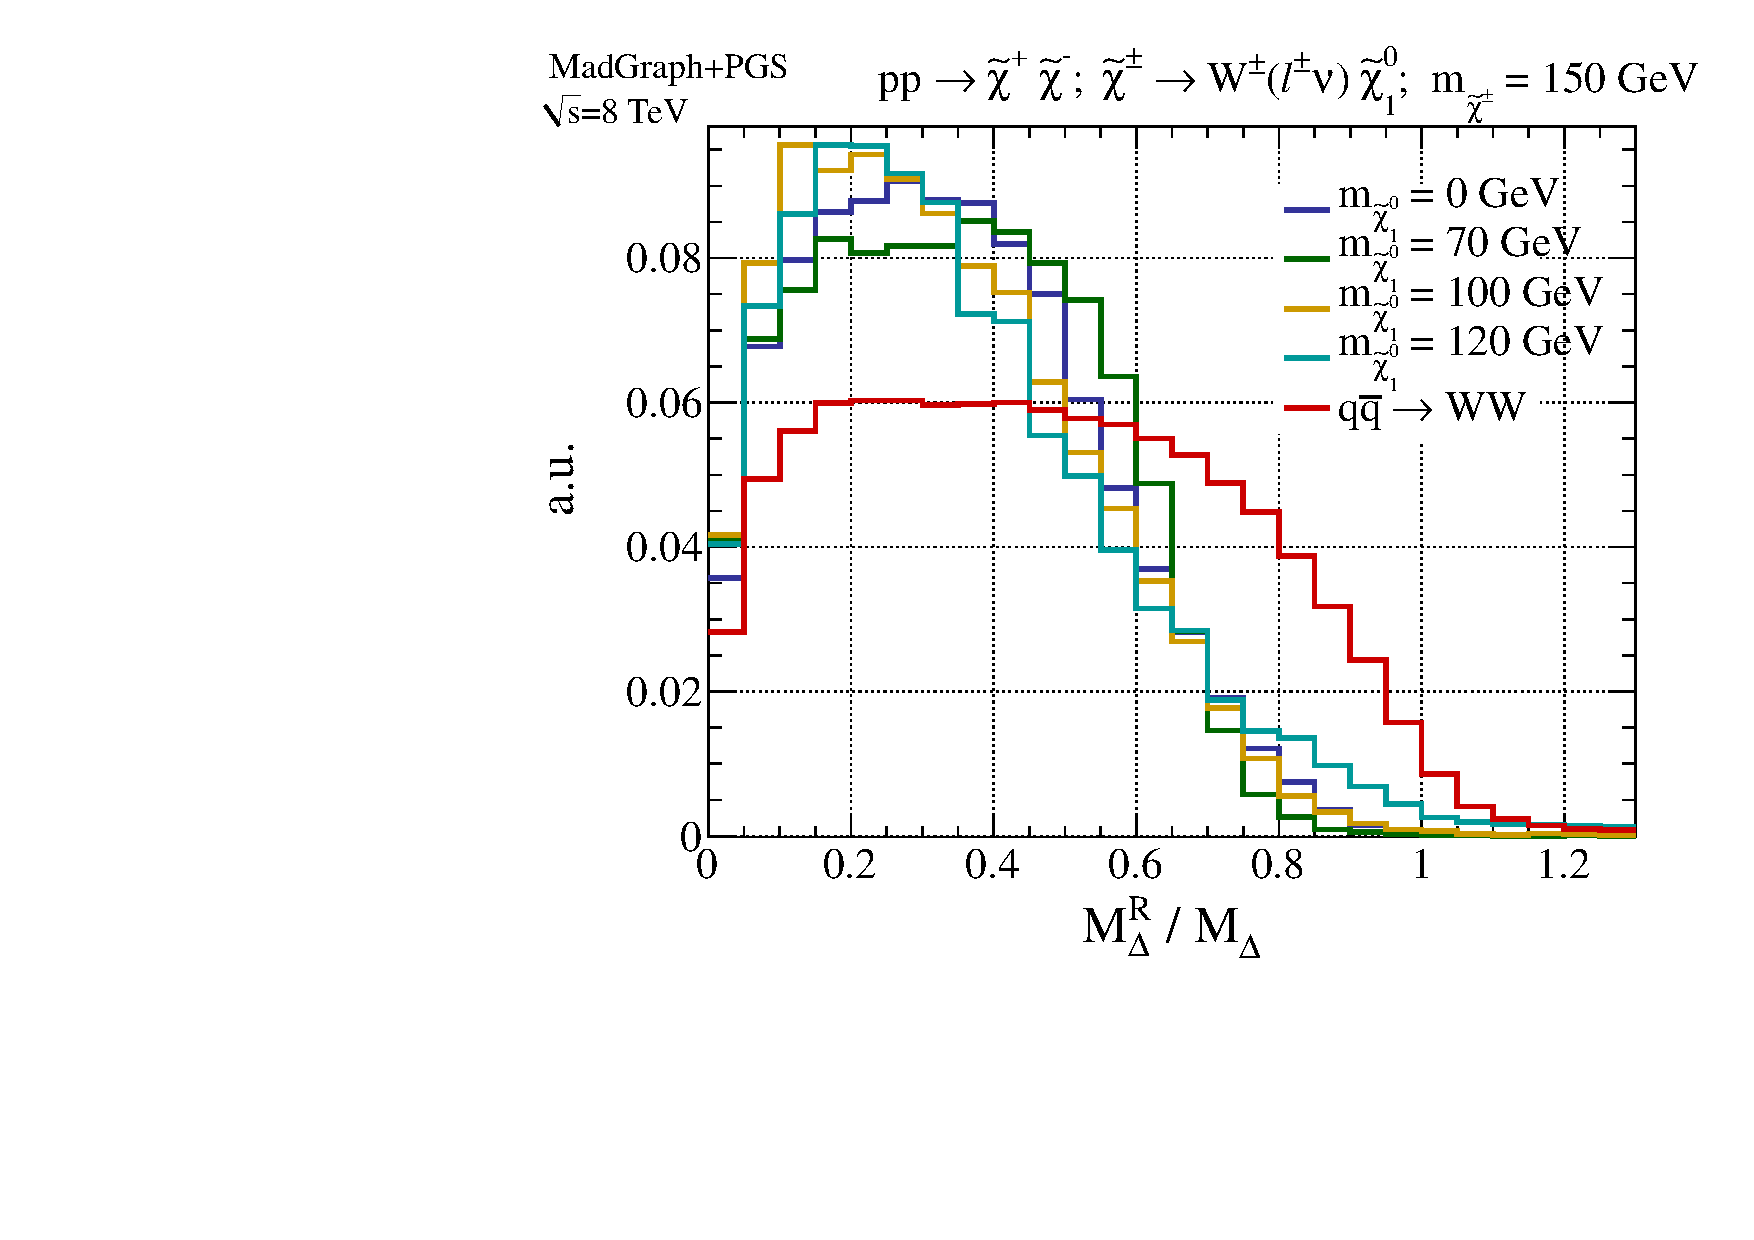
\includegraphics[width=0.35\columnwidth]{fig/sectionII/Mdelta_norm_1D_chargino.pdf}
\caption{Top Row: Distributions of $M_\Delta^R$ for a 150~GeV slepton (left) or chargino (right) and a range of neutralino masses. Also shown is the distribution of the $W^-W^+$ background. For the $W$ background, $M_\Delta = m_W$. Bottom row: Distributions of $M_\Delta^R$ normalized to $M_\Delta$ for selectrons (left) and charginos (right), again for a range of neutralino masses  \label{fig:compare_mdelta}}
\end{figure}

\begin{figure}[ht]
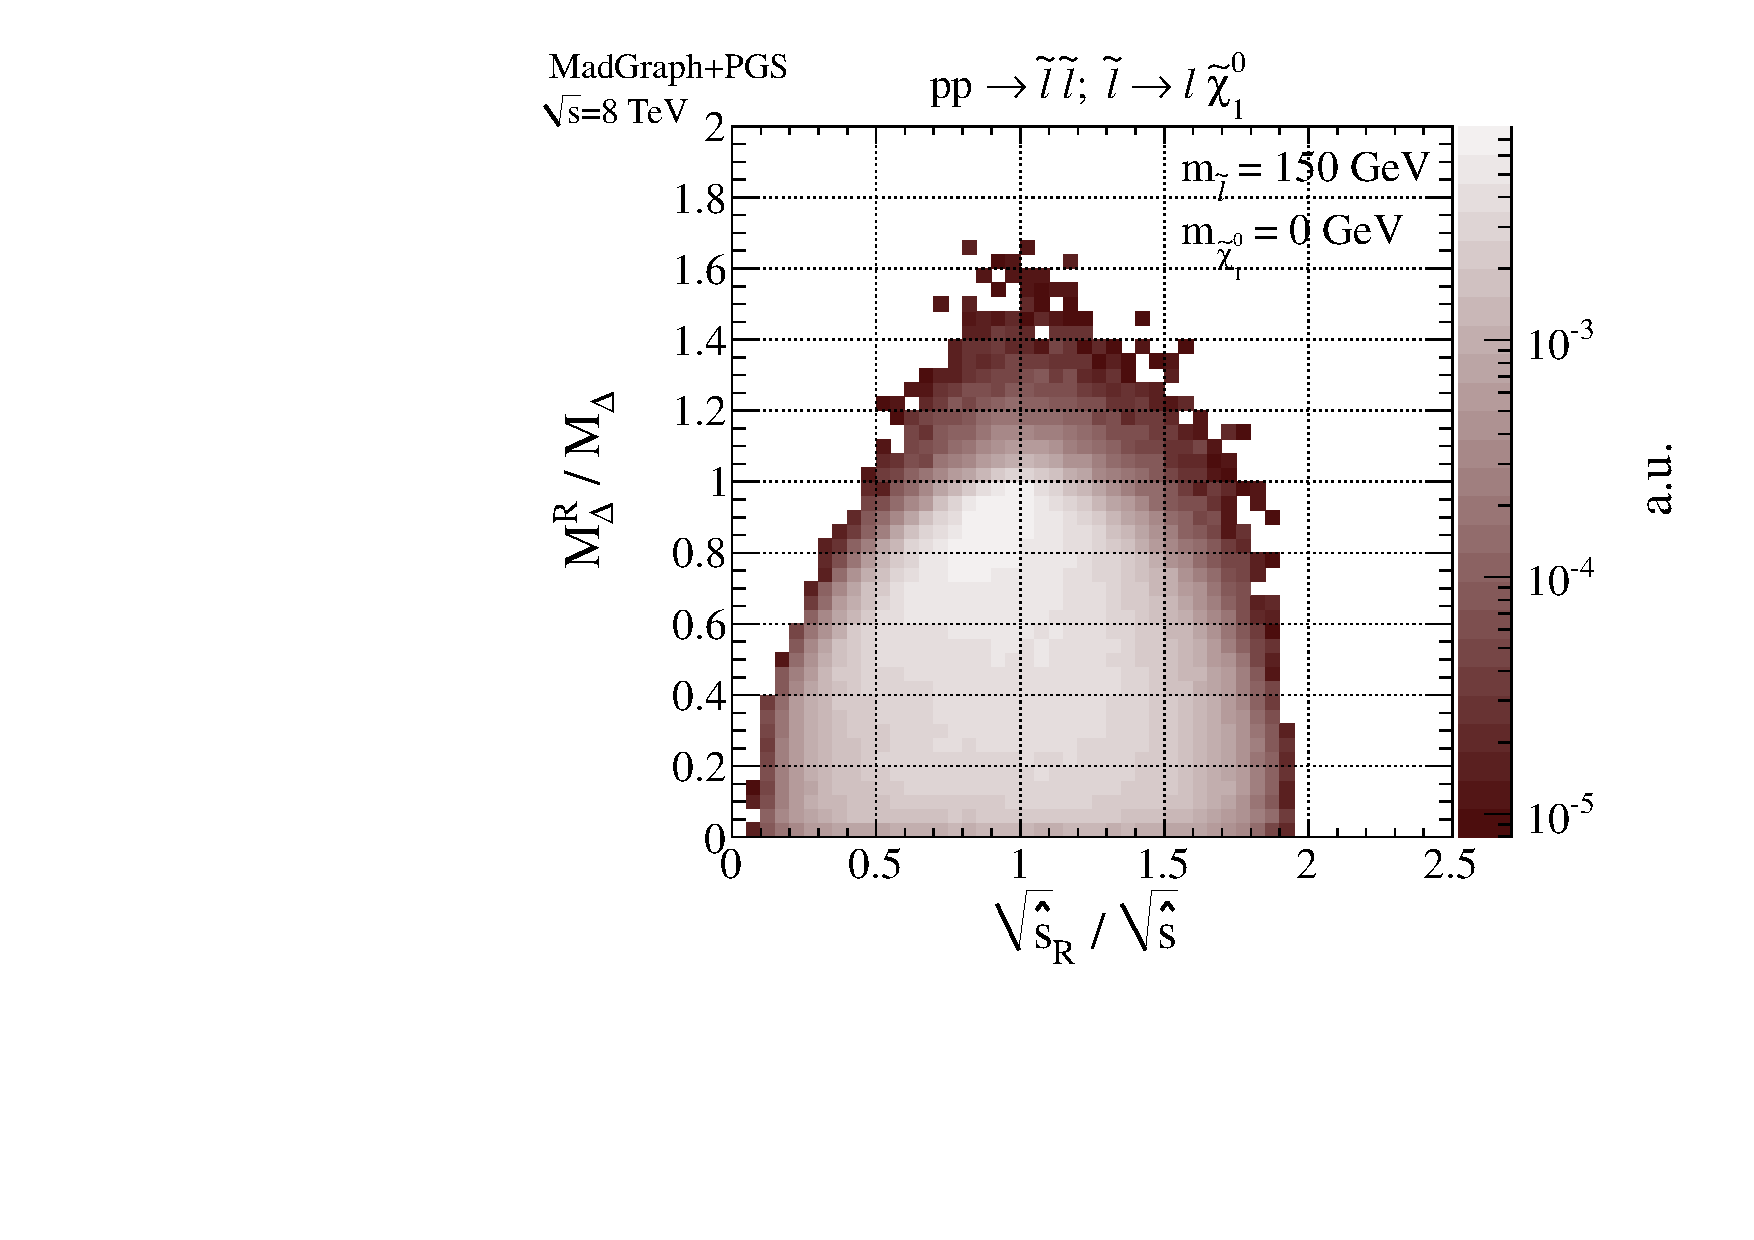
\includegraphics[width=0.32\columnwidth]{fig/sectionII/Mdelta_norm_v_shat_normtrue_slepton_150_0.pdf}
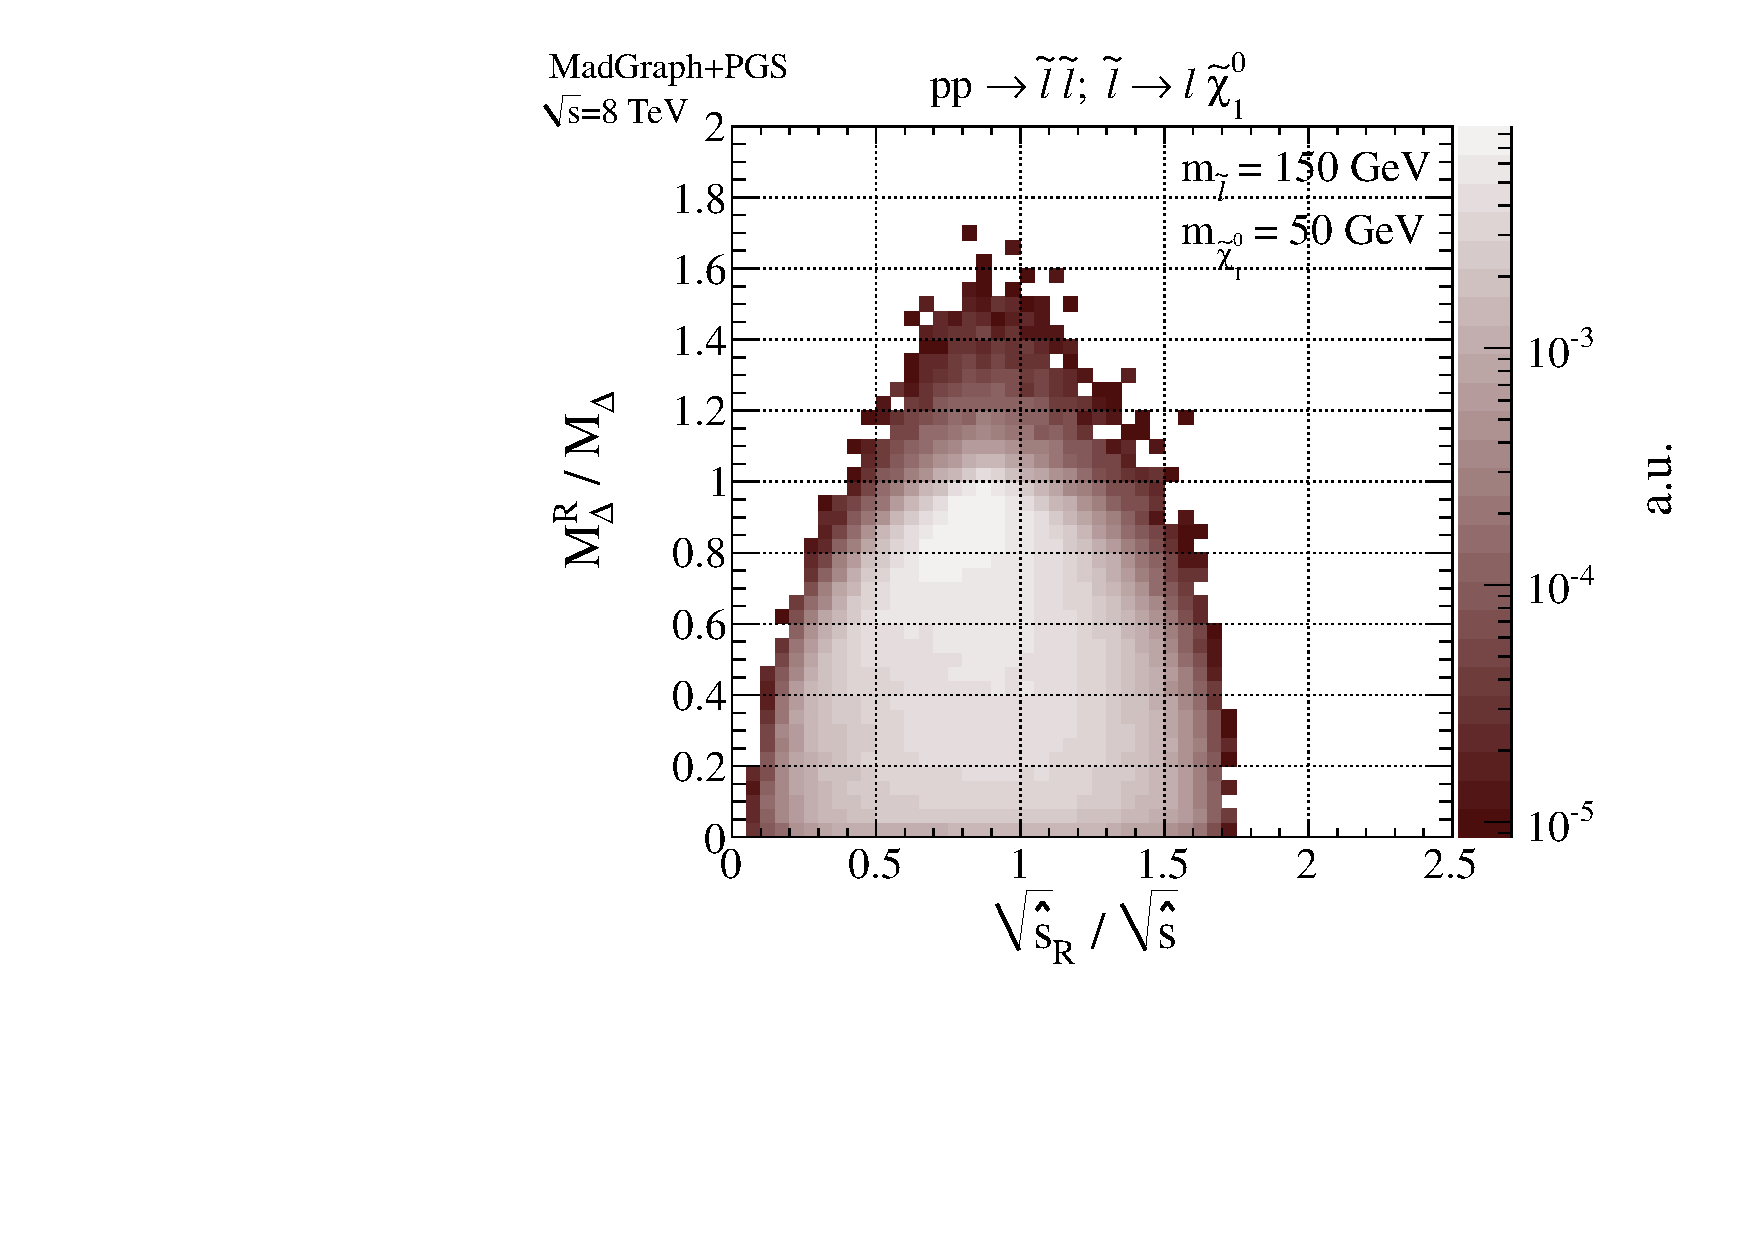
\includegraphics[width=0.32\columnwidth]{fig/sectionII/Mdelta_norm_v_shat_normtrue_slepton_150_50.pdf}
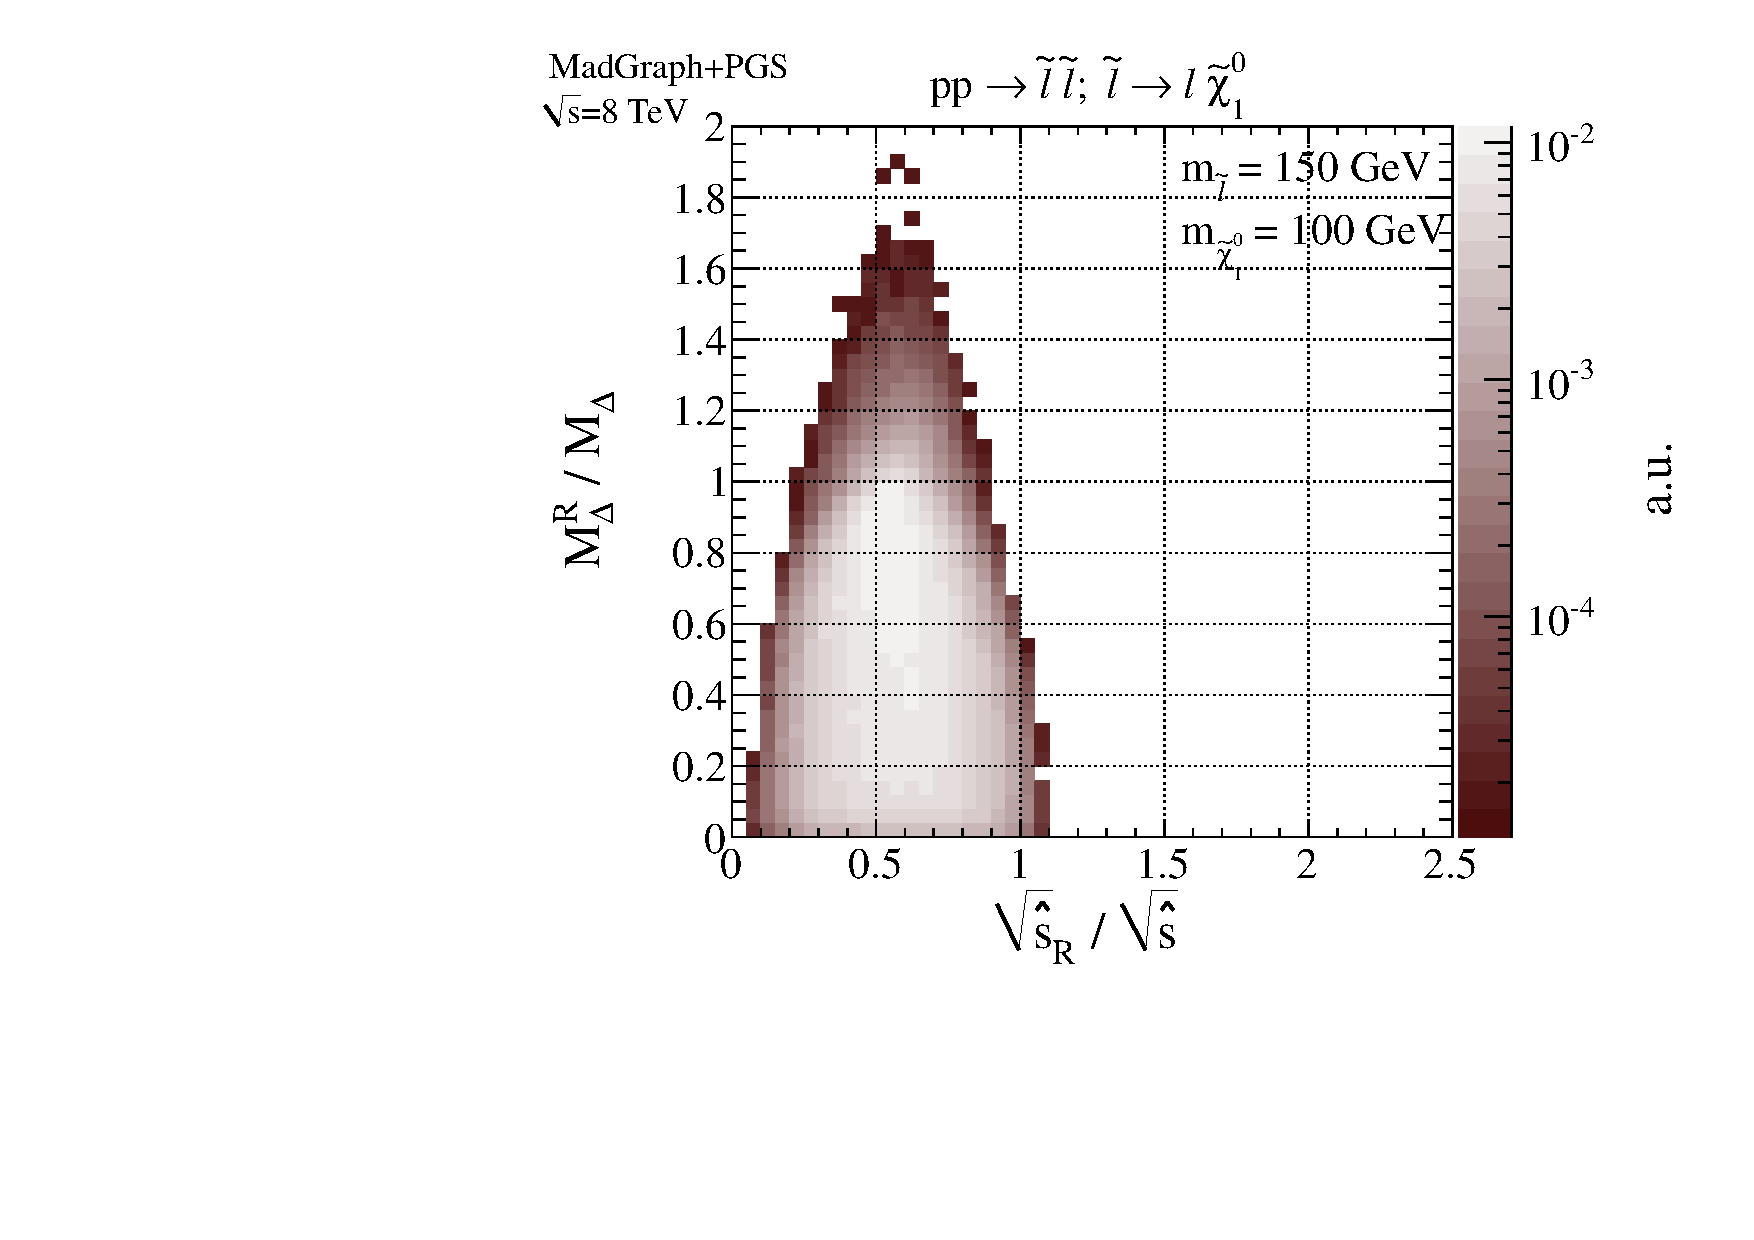
\includegraphics[width=0.32\columnwidth]{fig/sectionII/Mdelta_norm_v_shat_normtrue_slepton_150_100.pdf}
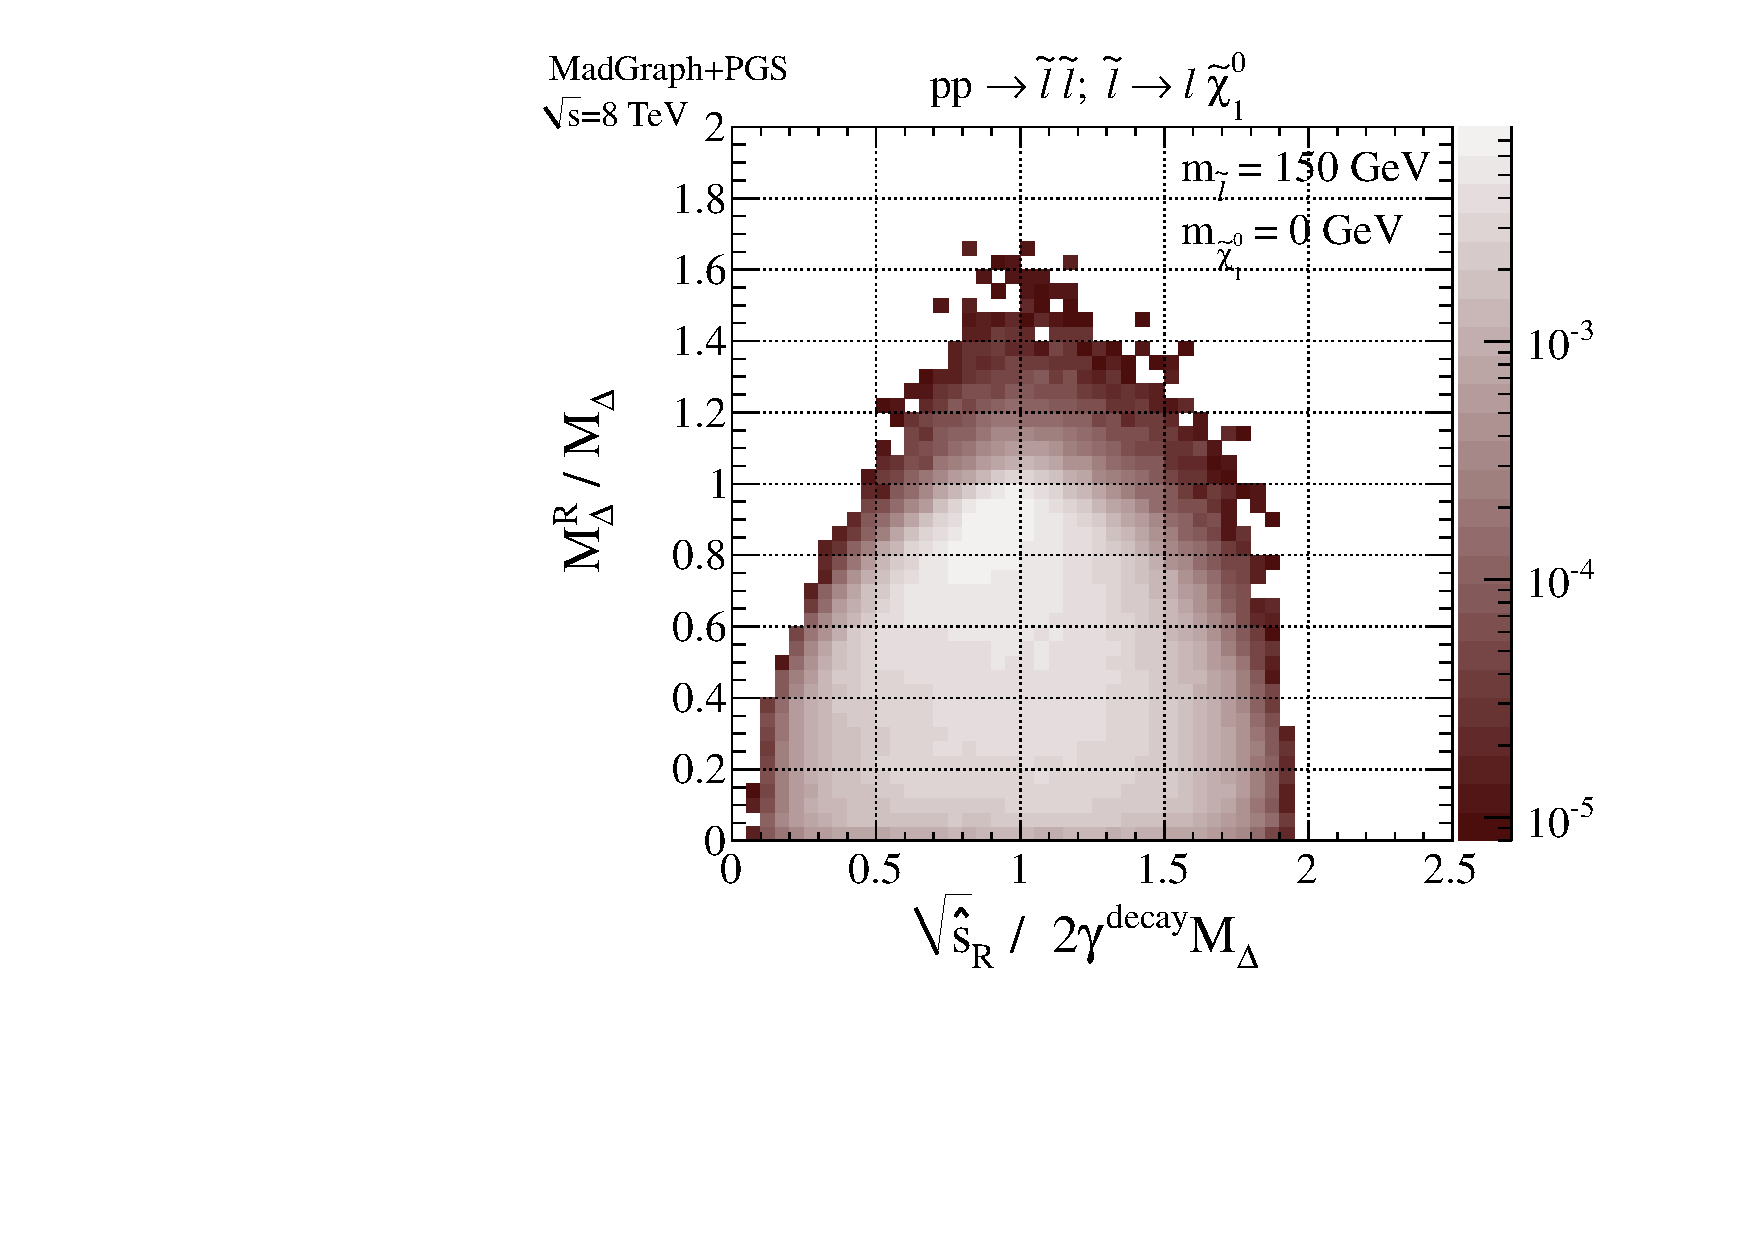
\includegraphics[width=0.32\columnwidth]{fig/sectionII/Mdelta_norm_v_shat_norm_slepton_150_0.pdf}
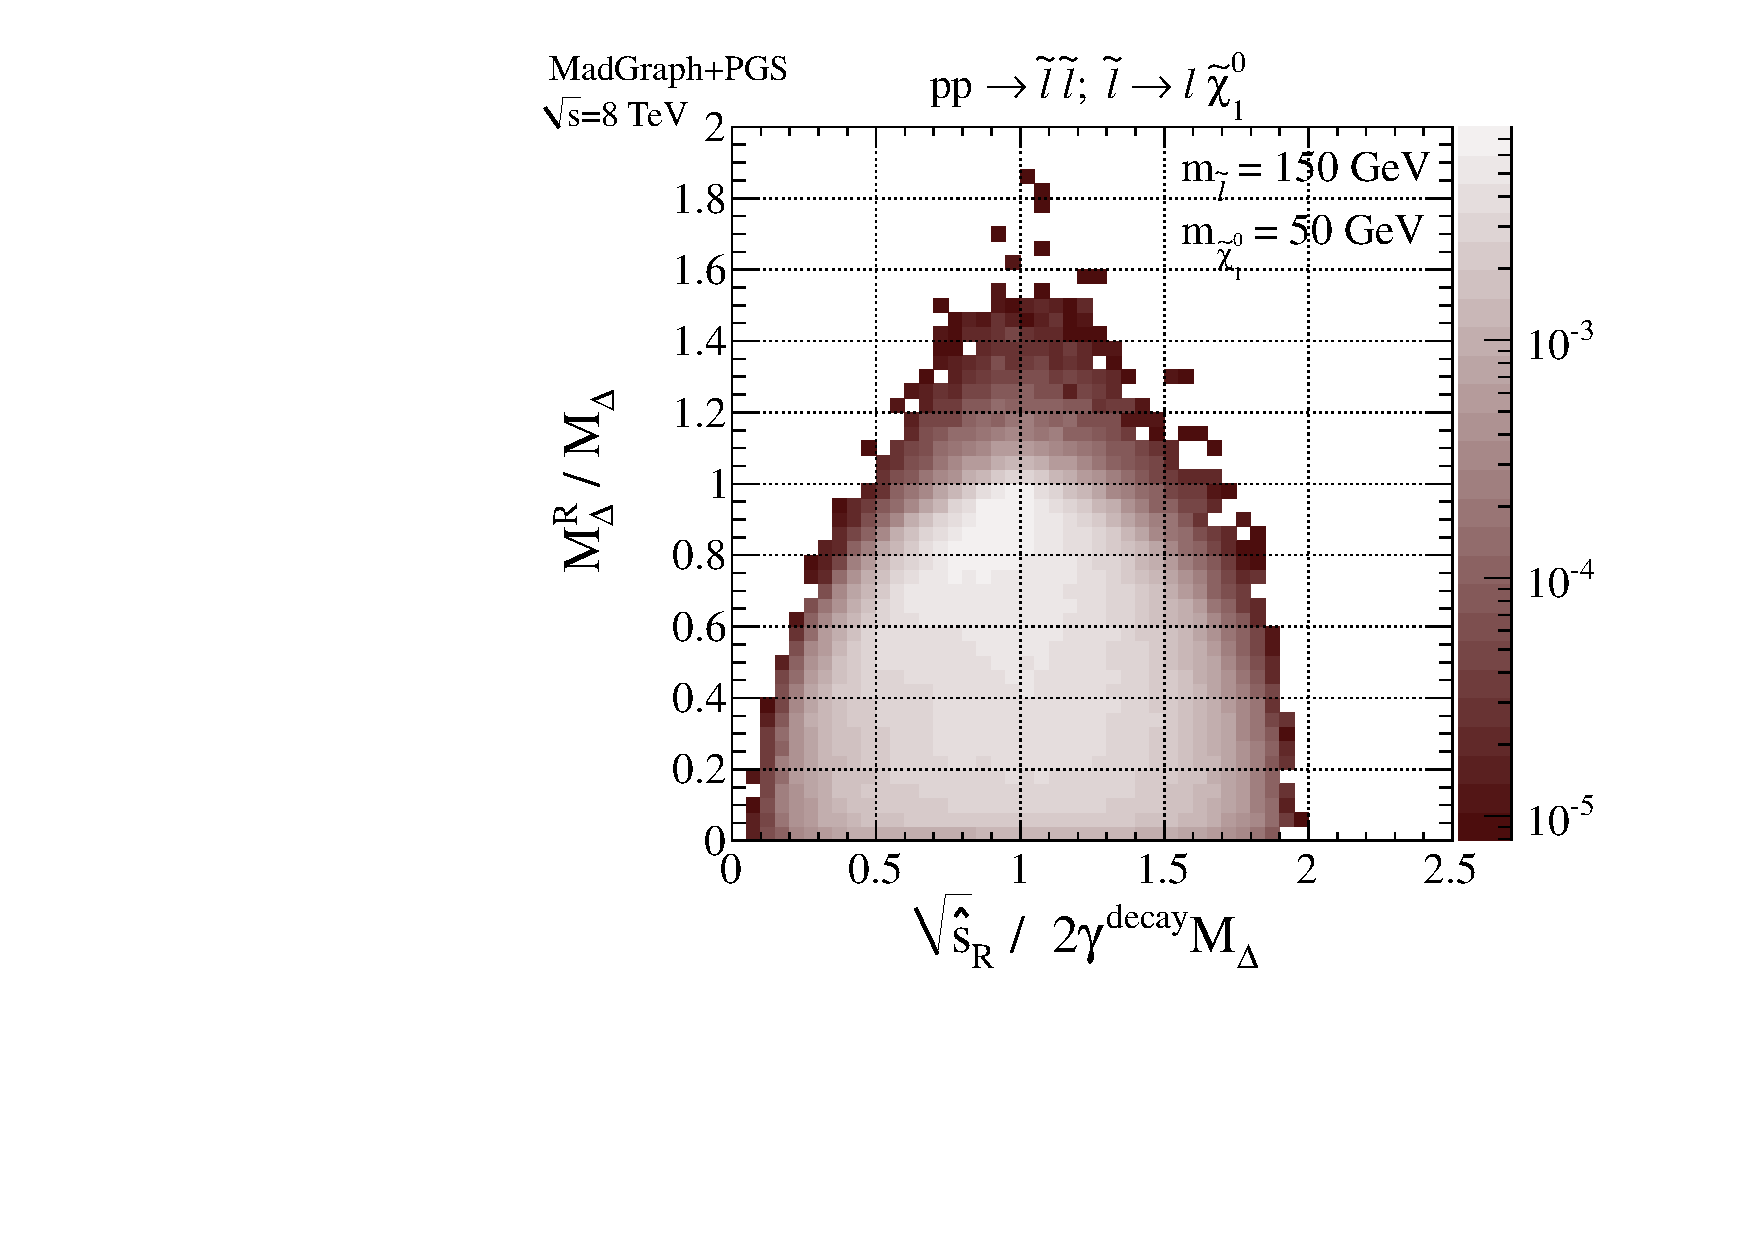
\includegraphics[width=0.32\columnwidth]{fig/sectionII/Mdelta_norm_v_shat_norm_slepton_150_50.pdf}
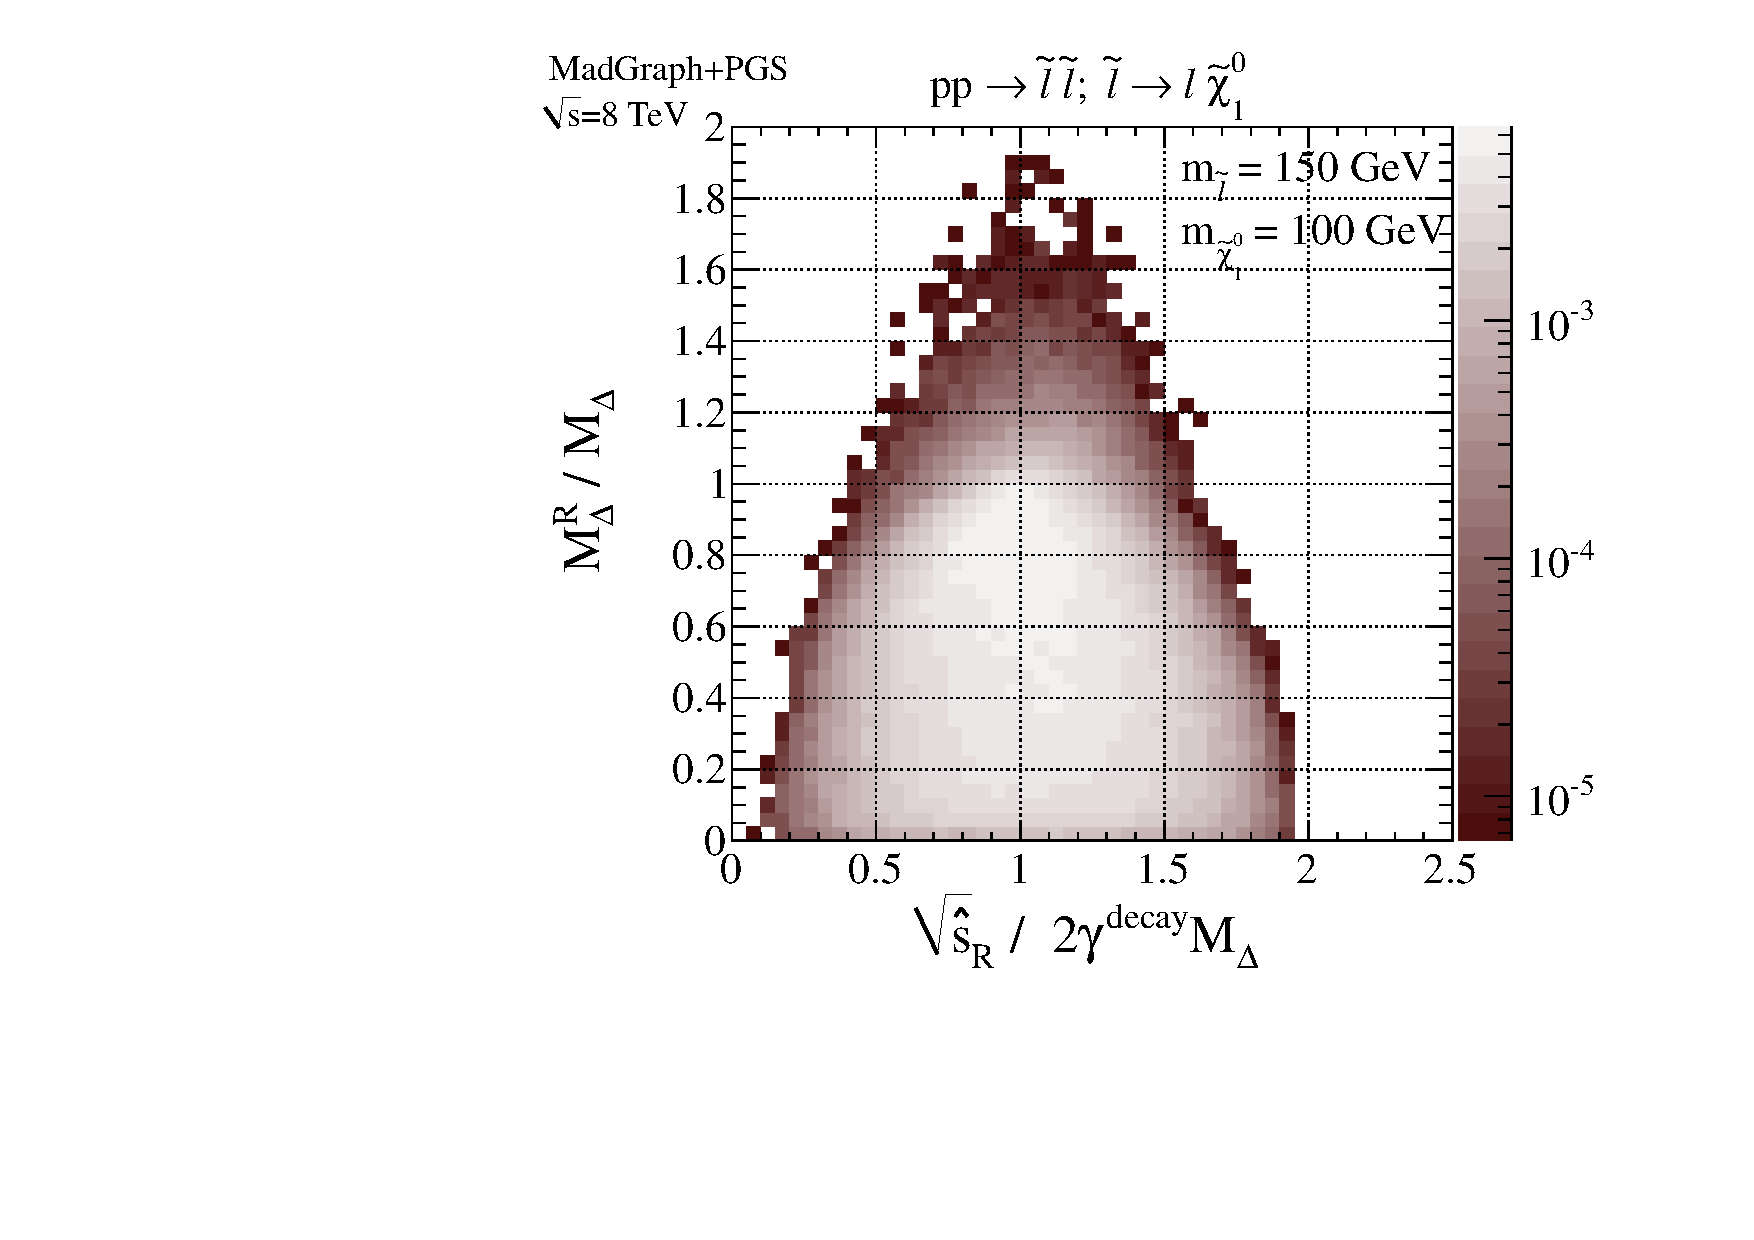
\includegraphics[width=0.32\columnwidth]{fig/sectionII/Mdelta_norm_v_shat_norm_slepton_150_100.pdf}
\caption{Top Row: Distributions of $\sqrt{\hat{s}}_R/\sqrt{\hat{s}}$ vs.~$M_\Delta^R/M_\Delta$ for 150~GeV sleptons and a range of $m_{\tilde{\chi}})$ masses. Bottom Row: Distributions of $\sqrt{\hat{s}}_R/2 \gamma^{\rm decay}M_\Delta$ vs.~$M_\Delta^R/M_\Delta$ for 150~GeV sleptons and a range of $m_{\tilde{\chi}})$ masses.  \label{fig:compare_shat_mdelta}}
\end{figure}

\begin{figure}[ht]
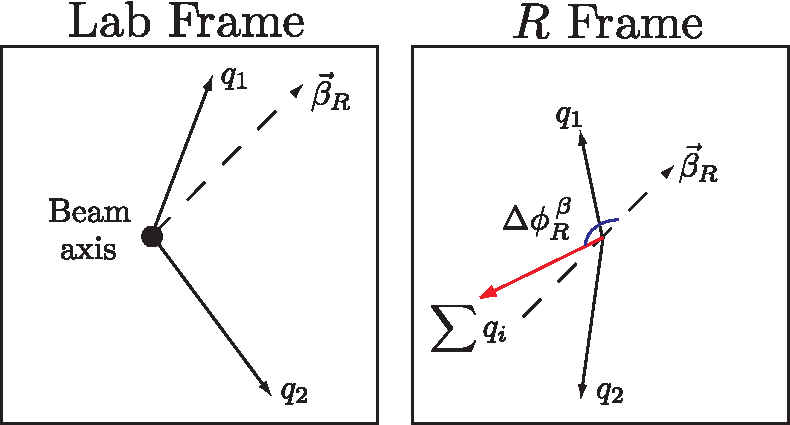
\includegraphics[width=0.7\columnwidth]{fig/sectionII/deltaphi.pdf}
\caption{Schematic example of the definition of the azimuthal angle $\Delta\phi_R^{\beta}$. The lab frame (seen here down the beam-line) contains two visible objects, $q_1$ and $q_2$. The direction of the boost $\vec{\beta}_R$ (defined in Eq.~\eqref{eq:razorbeta}), in the lab frame is also shown. In the frame $R$, arrived at by performing the boost $\vec{\beta}_R$, the visible momenta $q_1$ and $q_2$ are shown, along with their sum. The azimuthal angle between their sum $q_1+q_2$ and the boost direction $\vec{\beta}_R$ in frame $R$ defines $\Delta \phi_R^{\beta}$. \label{fig:deltaphi}}
\end{figure}

\begin{figure}[ht]
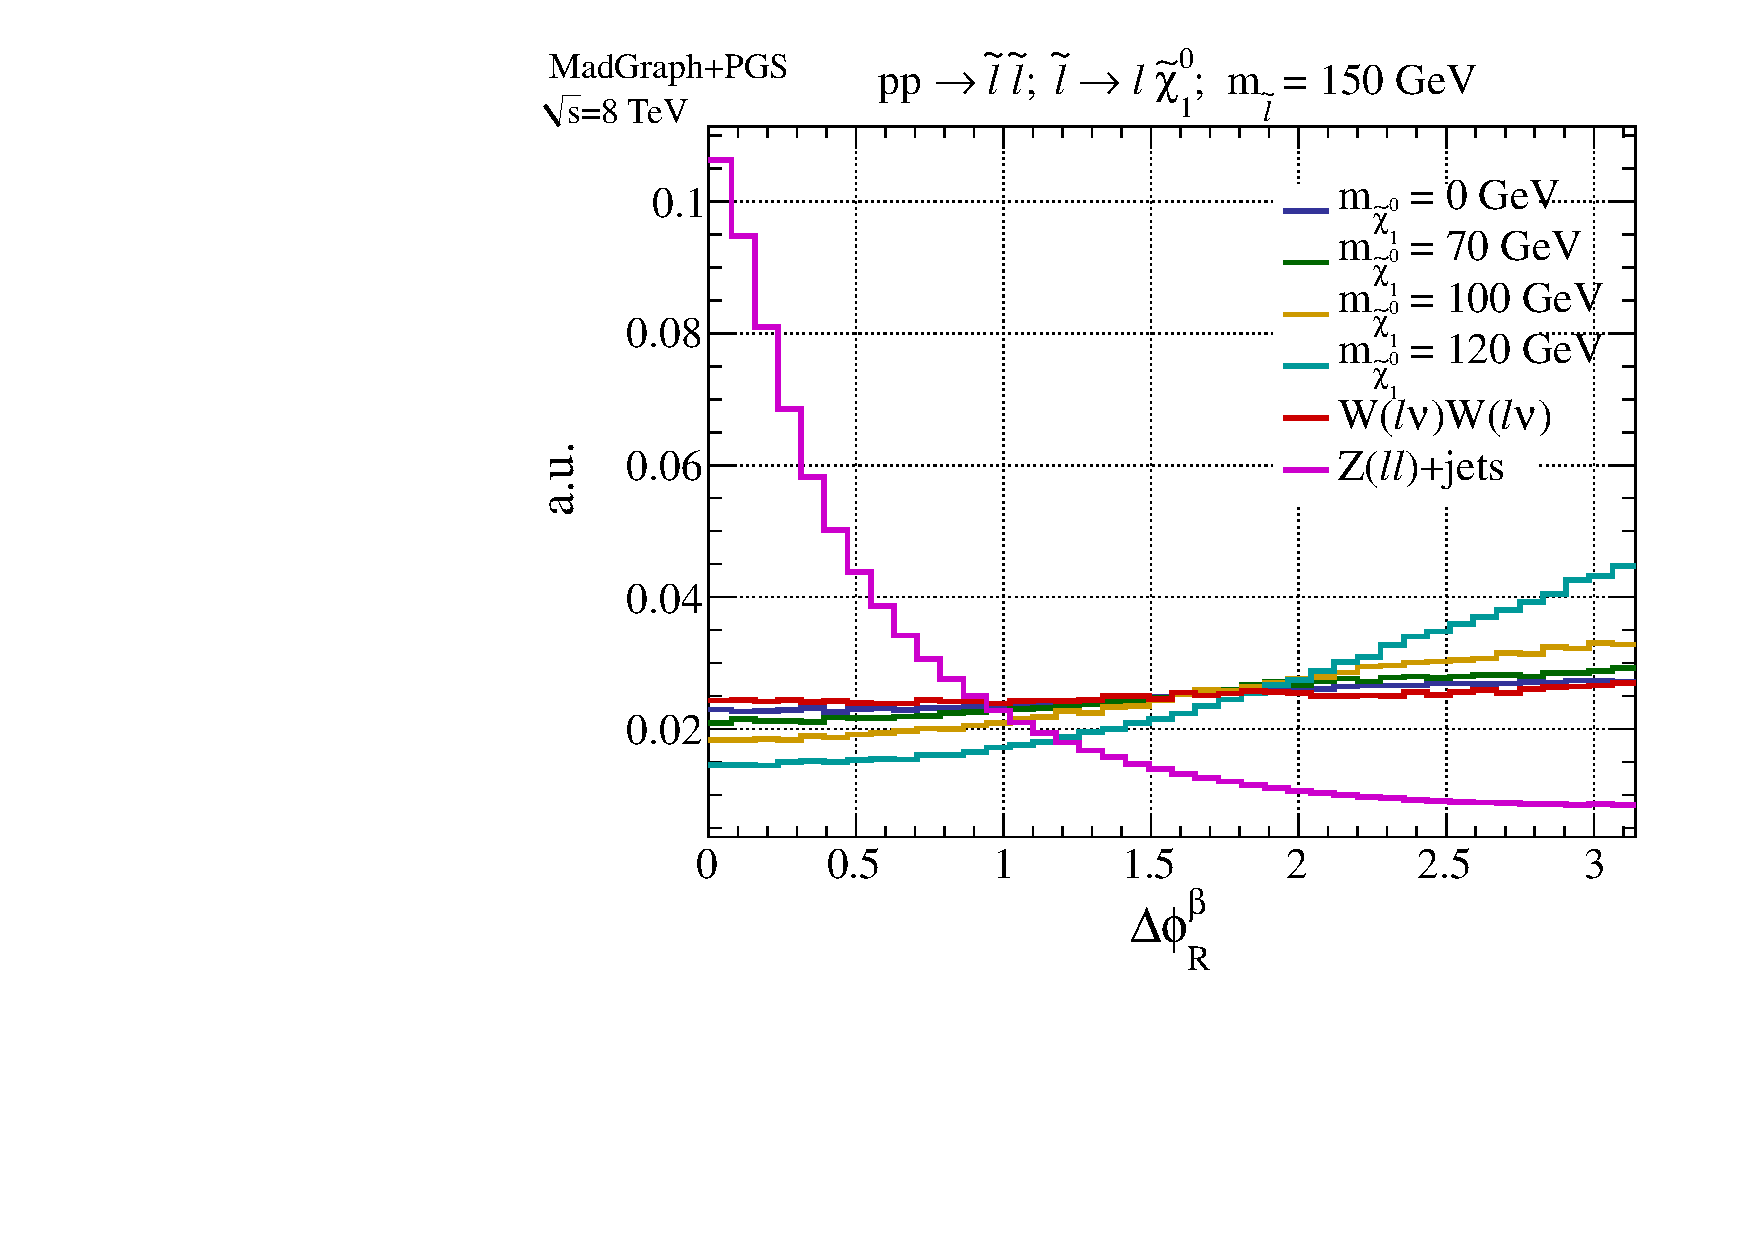
\includegraphics[width=0.45\columnwidth]{fig/sectionII/dphi_slepton.pdf}
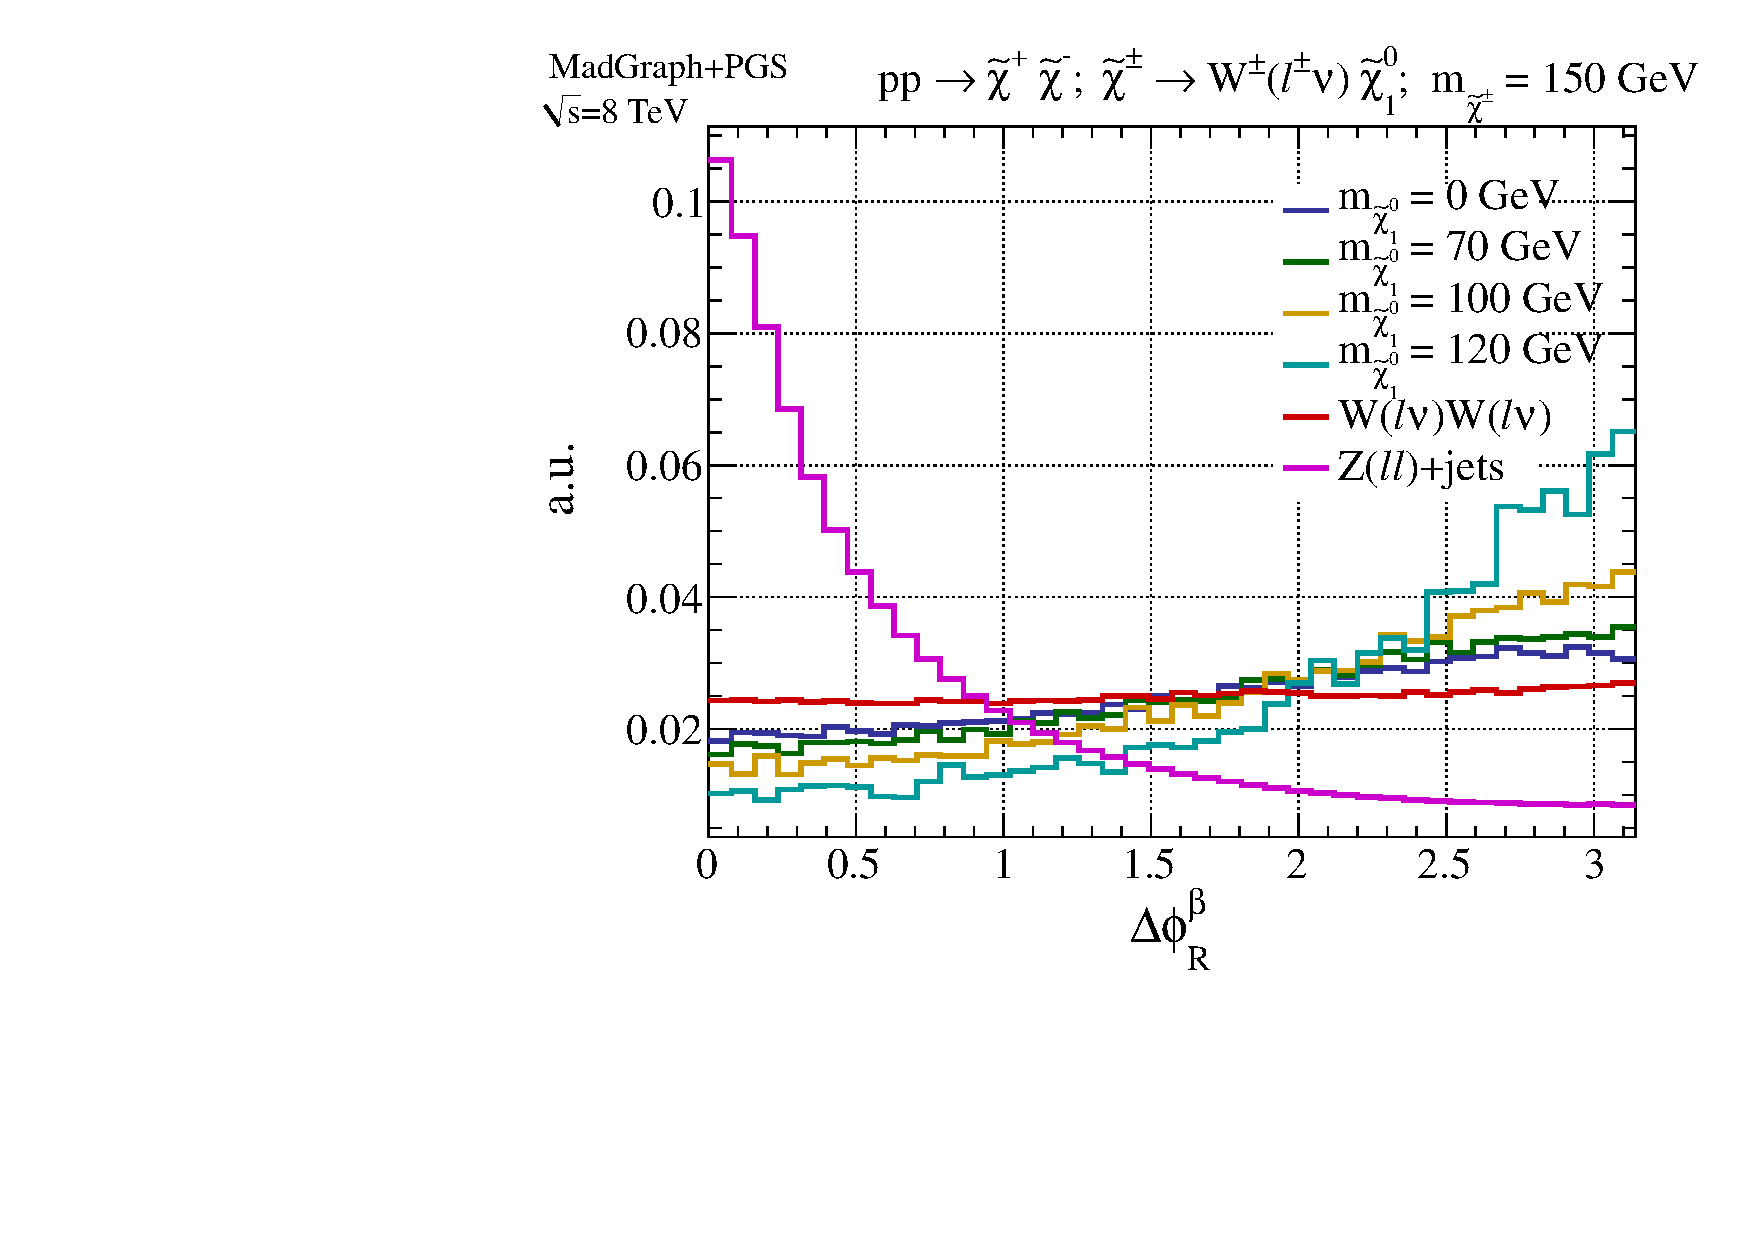
\includegraphics[width=0.45\columnwidth]{fig/sectionII/dphi_chargino.pdf}
\caption{Distributions of $\Delta\phi_R^\beta$ for a 150~GeV slepton (left) or chargino (right) and a range of neutralino masses. Also shown are the distributions of the $W^-W^+$ and Drell-Yan $Z$ backgrounds.  \label{fig:deltaRbeta}}
\end{figure}

\begin{figure}[ht]
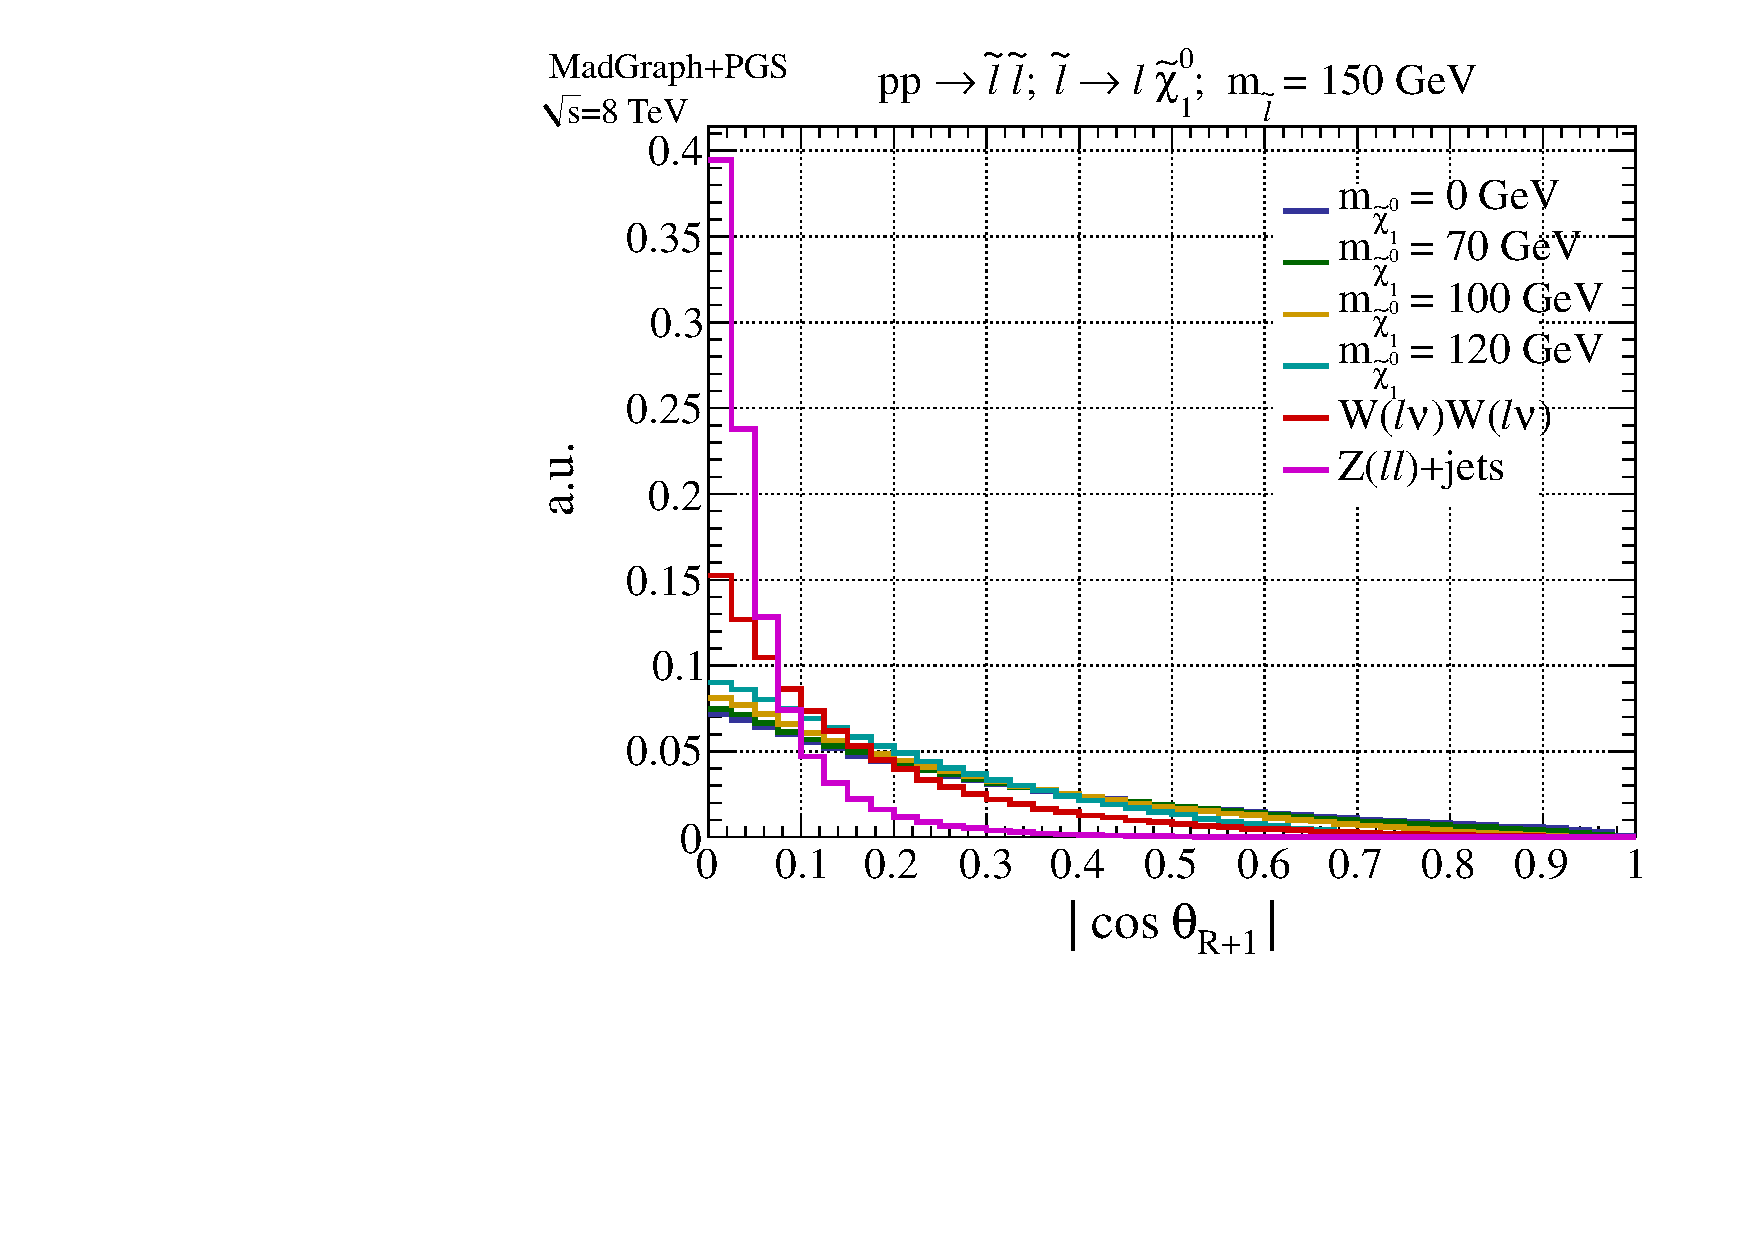
\includegraphics[width=0.45\columnwidth]{fig/sectionII/costheta_slepton.pdf}
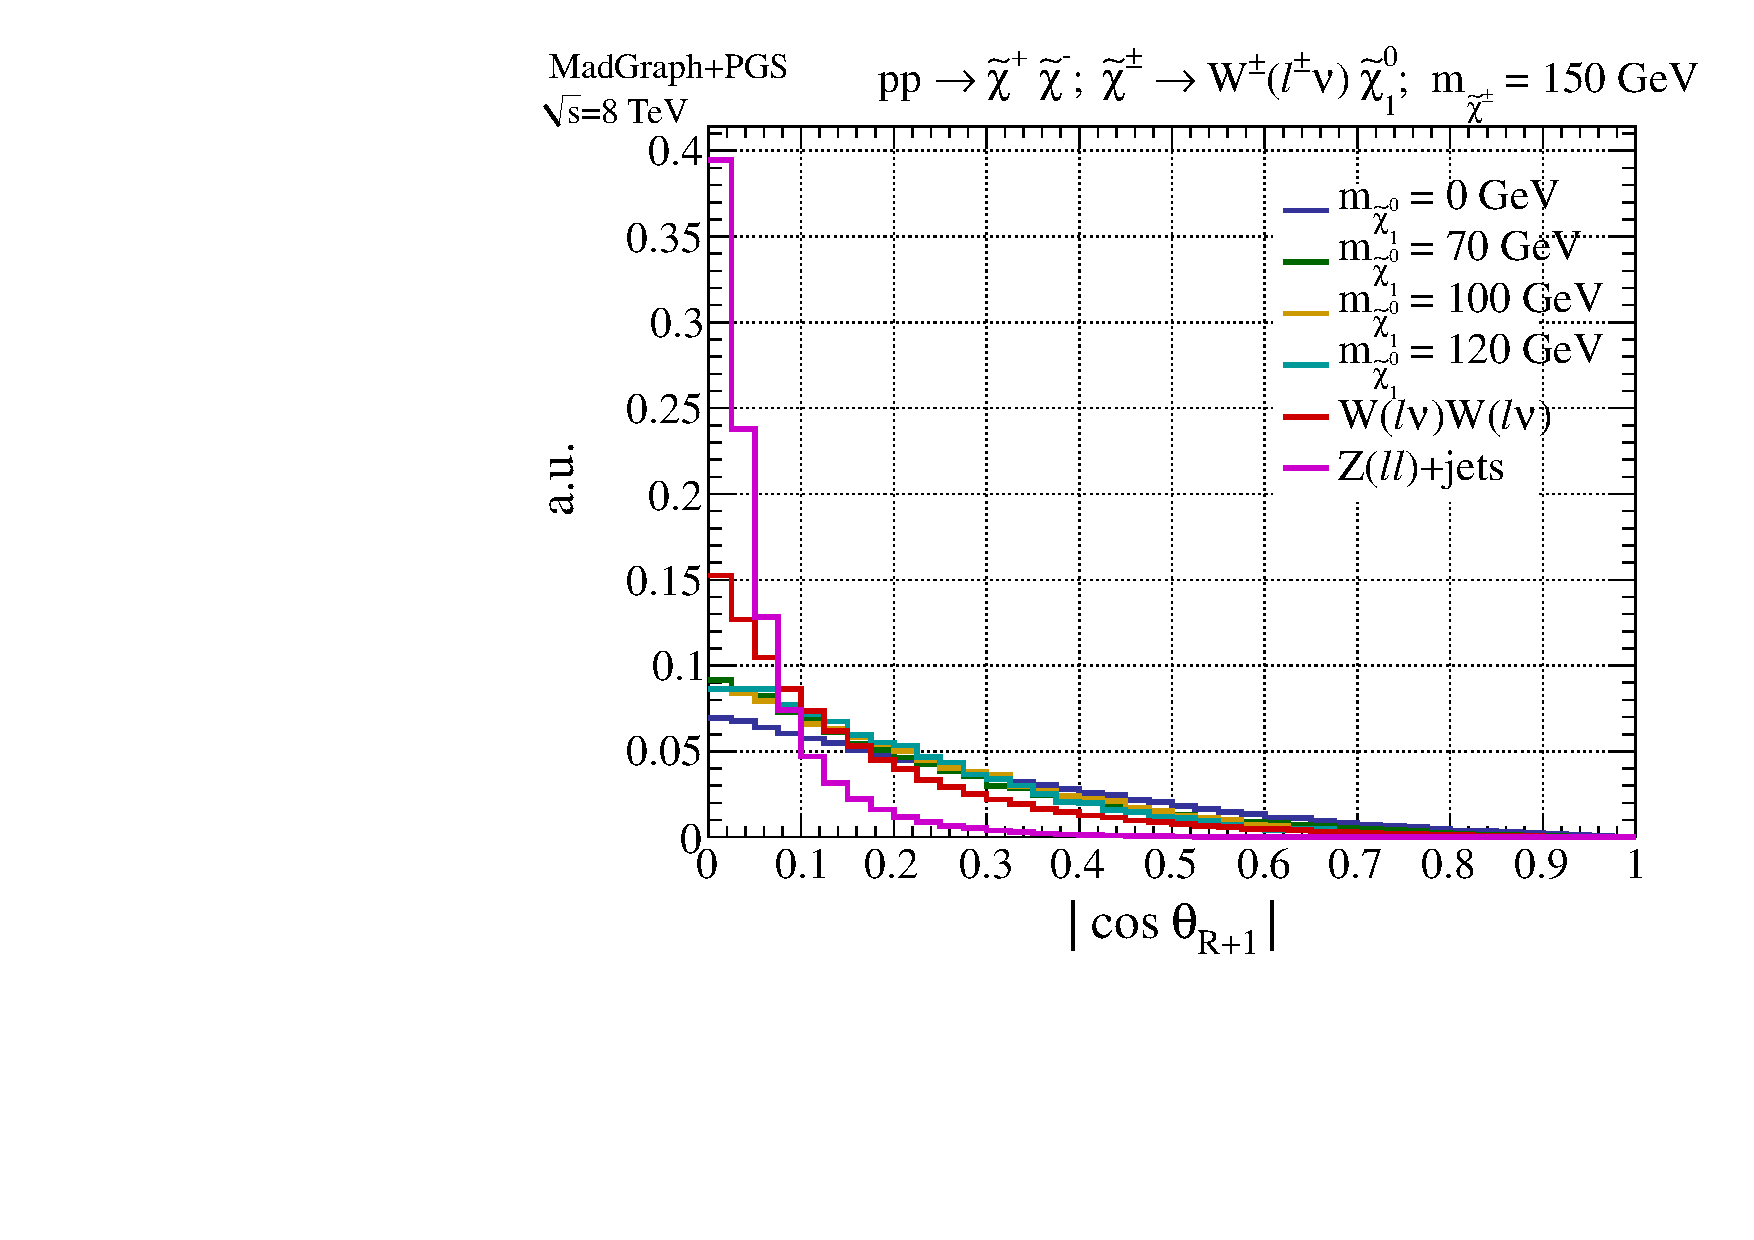
\includegraphics[width=0.45\columnwidth]{fig/sectionII/costheta_chargino.pdf}
\caption{Distribution of $|\cos\theta_{R+1}|$ for 150 GeV selectron (left) and chargino (right) pair production, decaying into a range of neutralino masses. Also shown are the $W^-W^+$ and Drell-Yan $Z$ background distributions. \label{fig:costheta}}
\end{figure}

\begin{figure}[ht]
%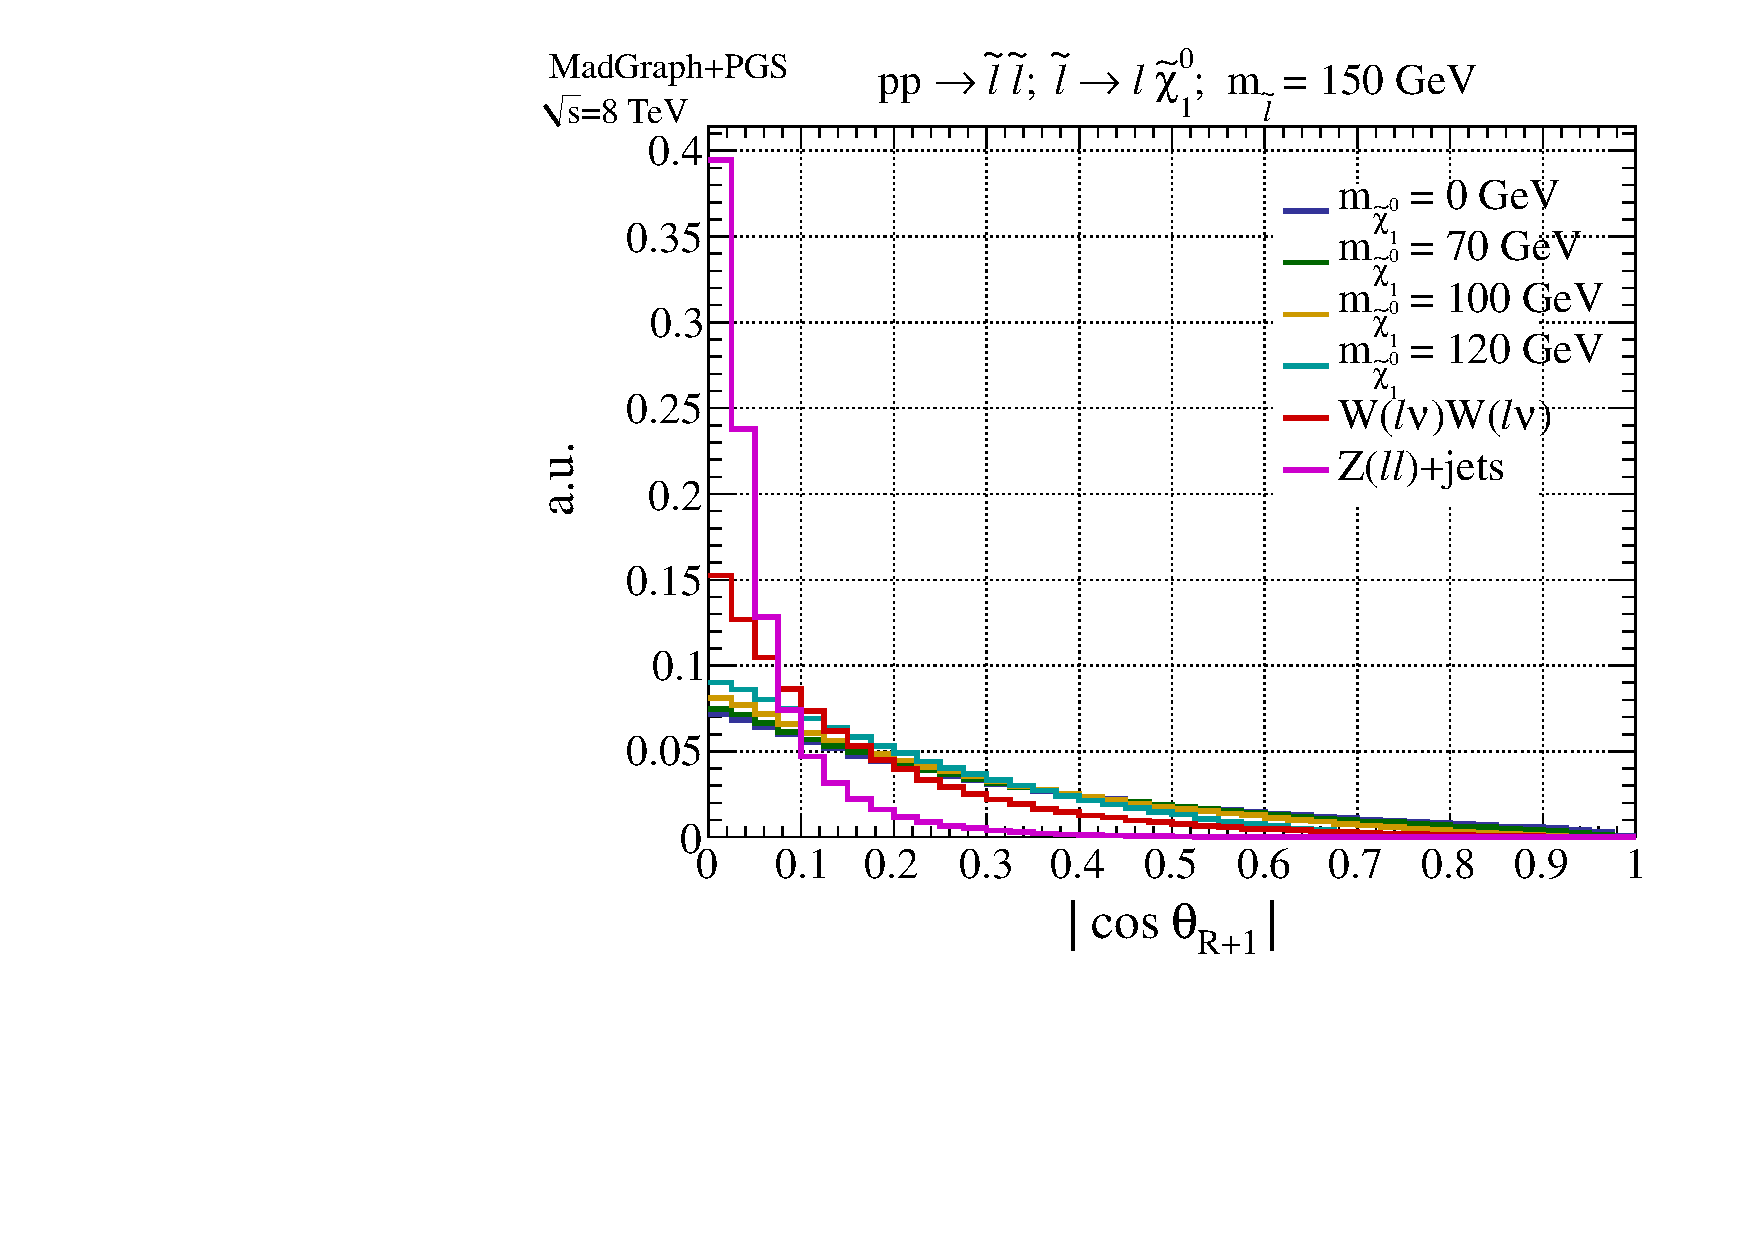
\includegraphics[width=0.4\columnwidth]{fig/sectionII/costheta_slepton.pdf}
%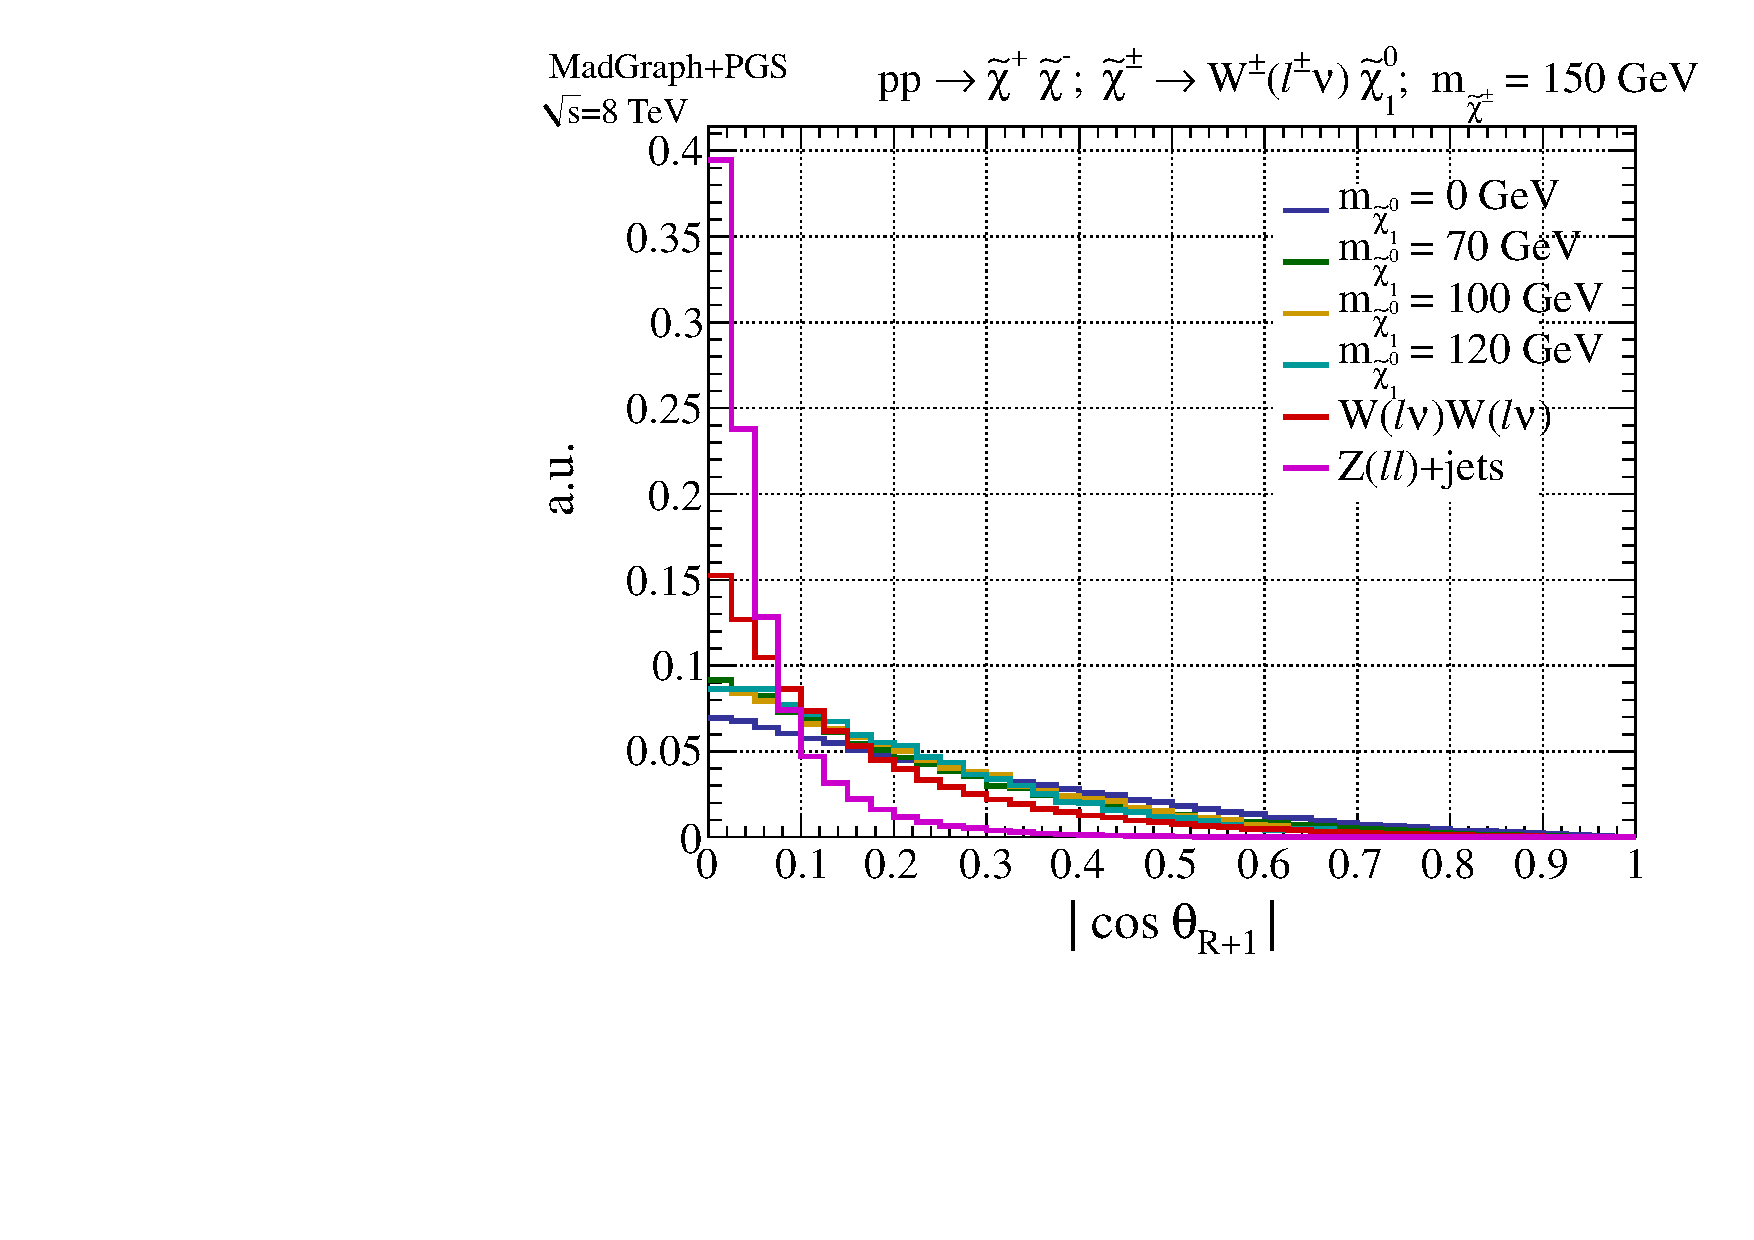
\includegraphics[width=0.4\columnwidth]{fig/sectionII/costheta_chargino.pdf}
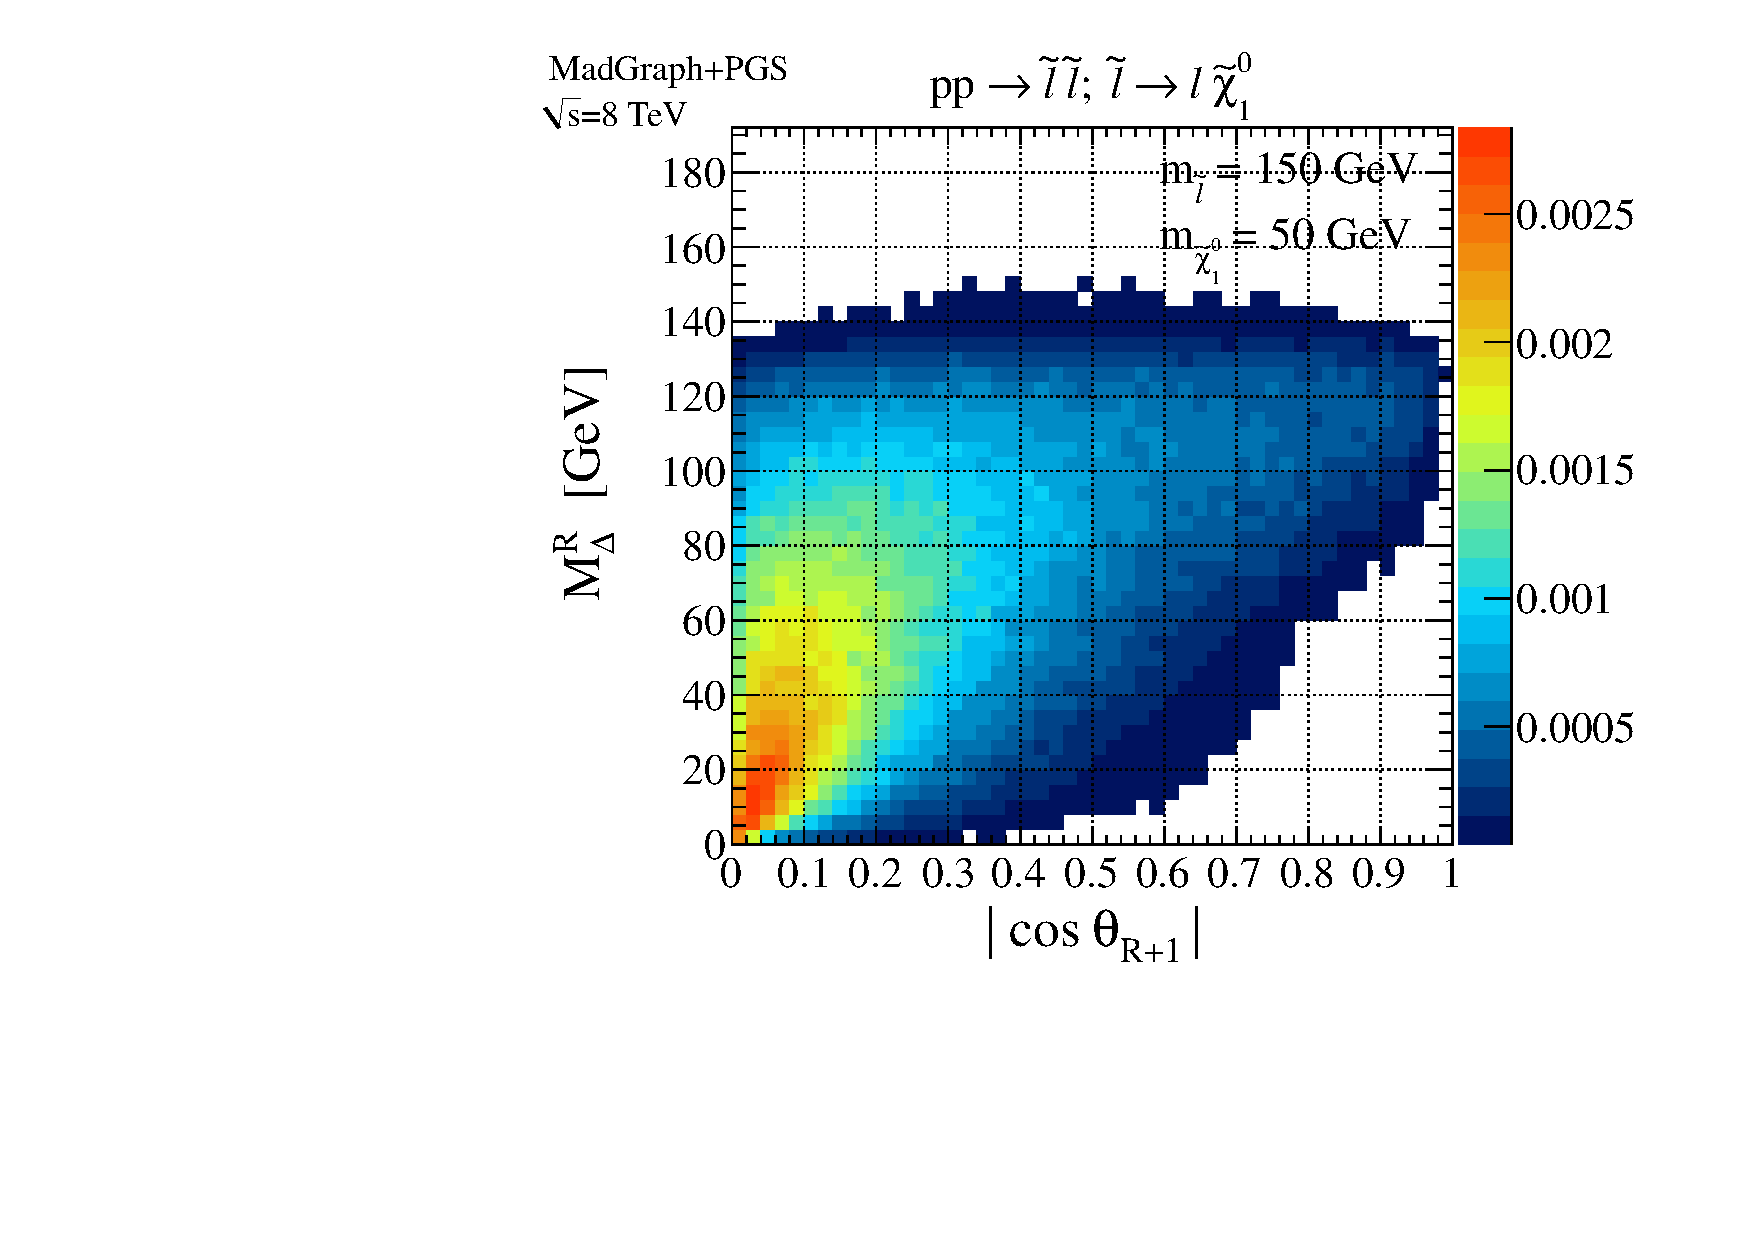
\includegraphics[width=0.35\columnwidth]{fig/sectionII/Mdelta_v_costheta_slepton_150_50.pdf}
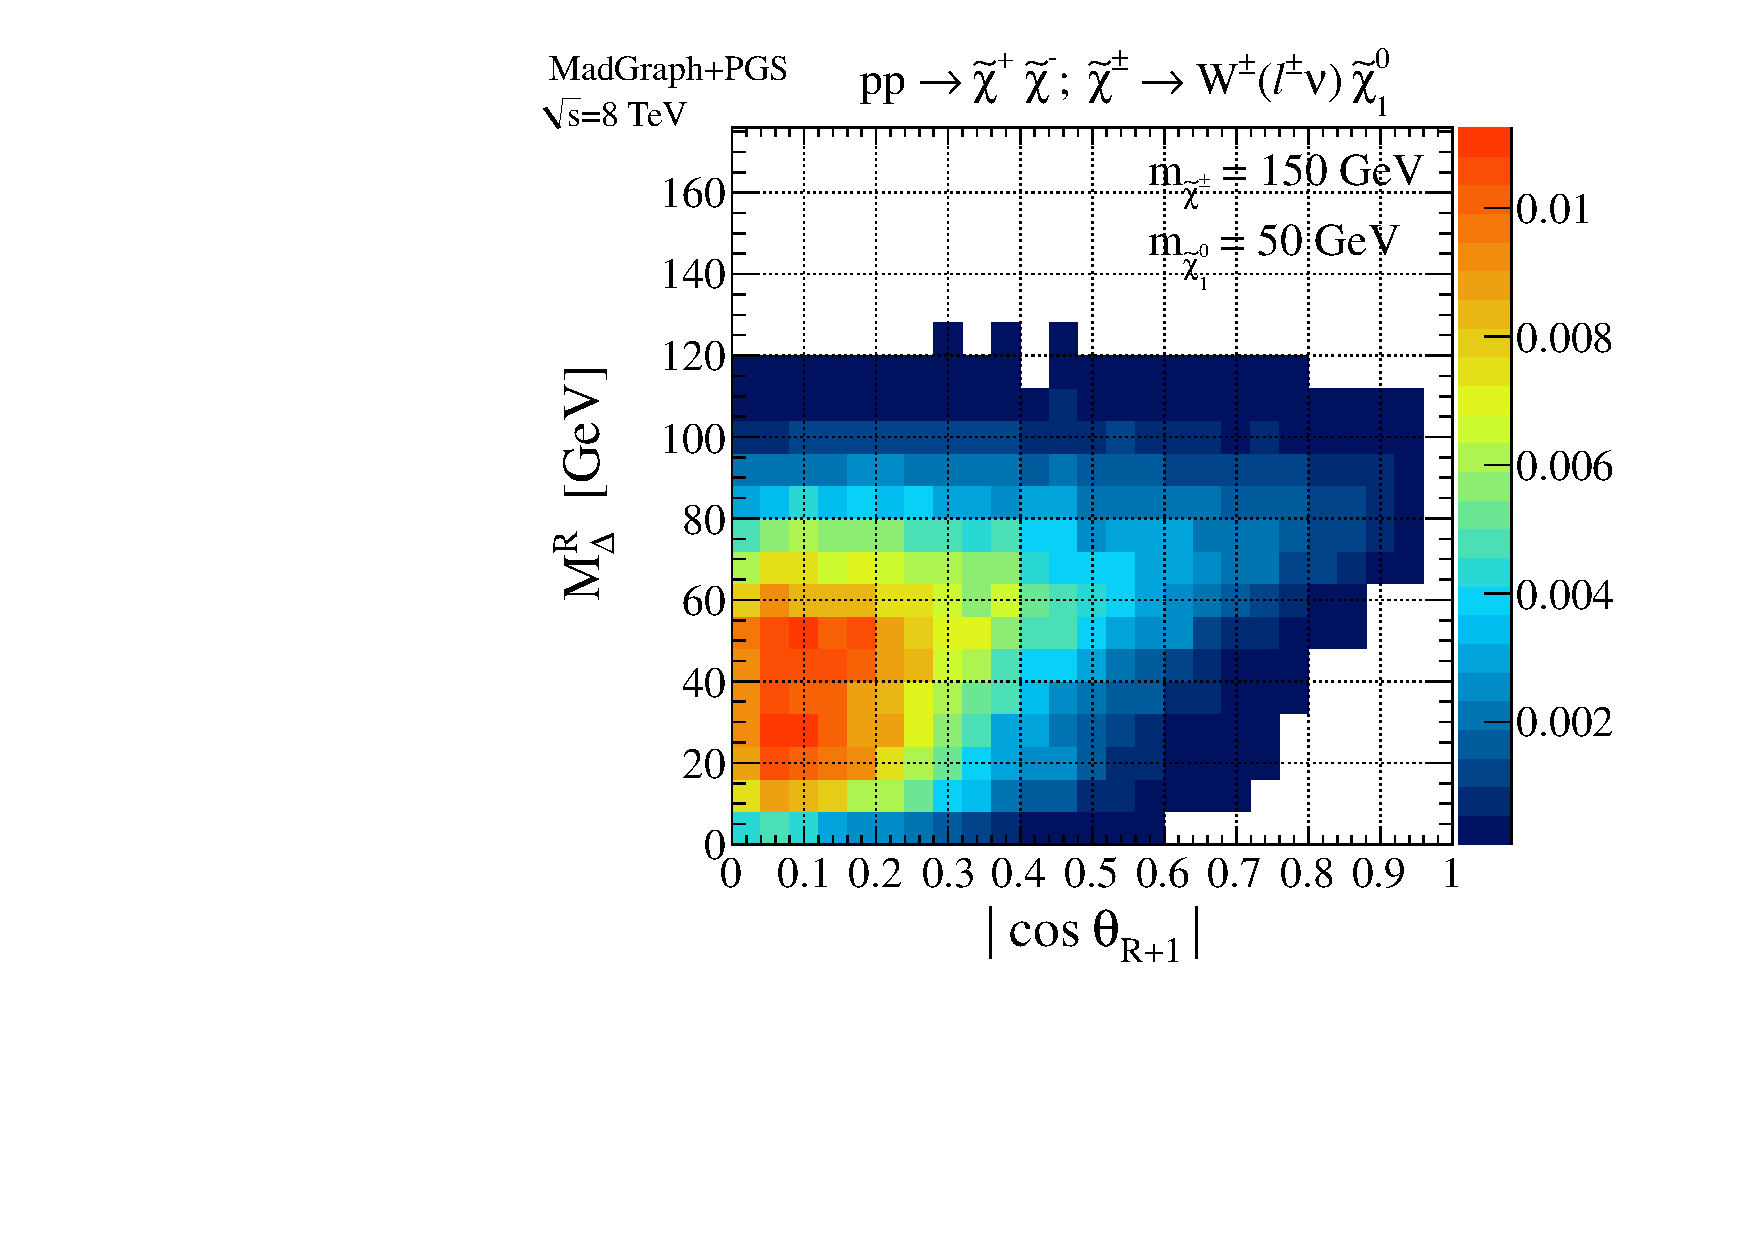
\includegraphics[width=0.35\columnwidth]{fig/sectionII/Mdelta_v_costheta_chargino_150_50.pdf}
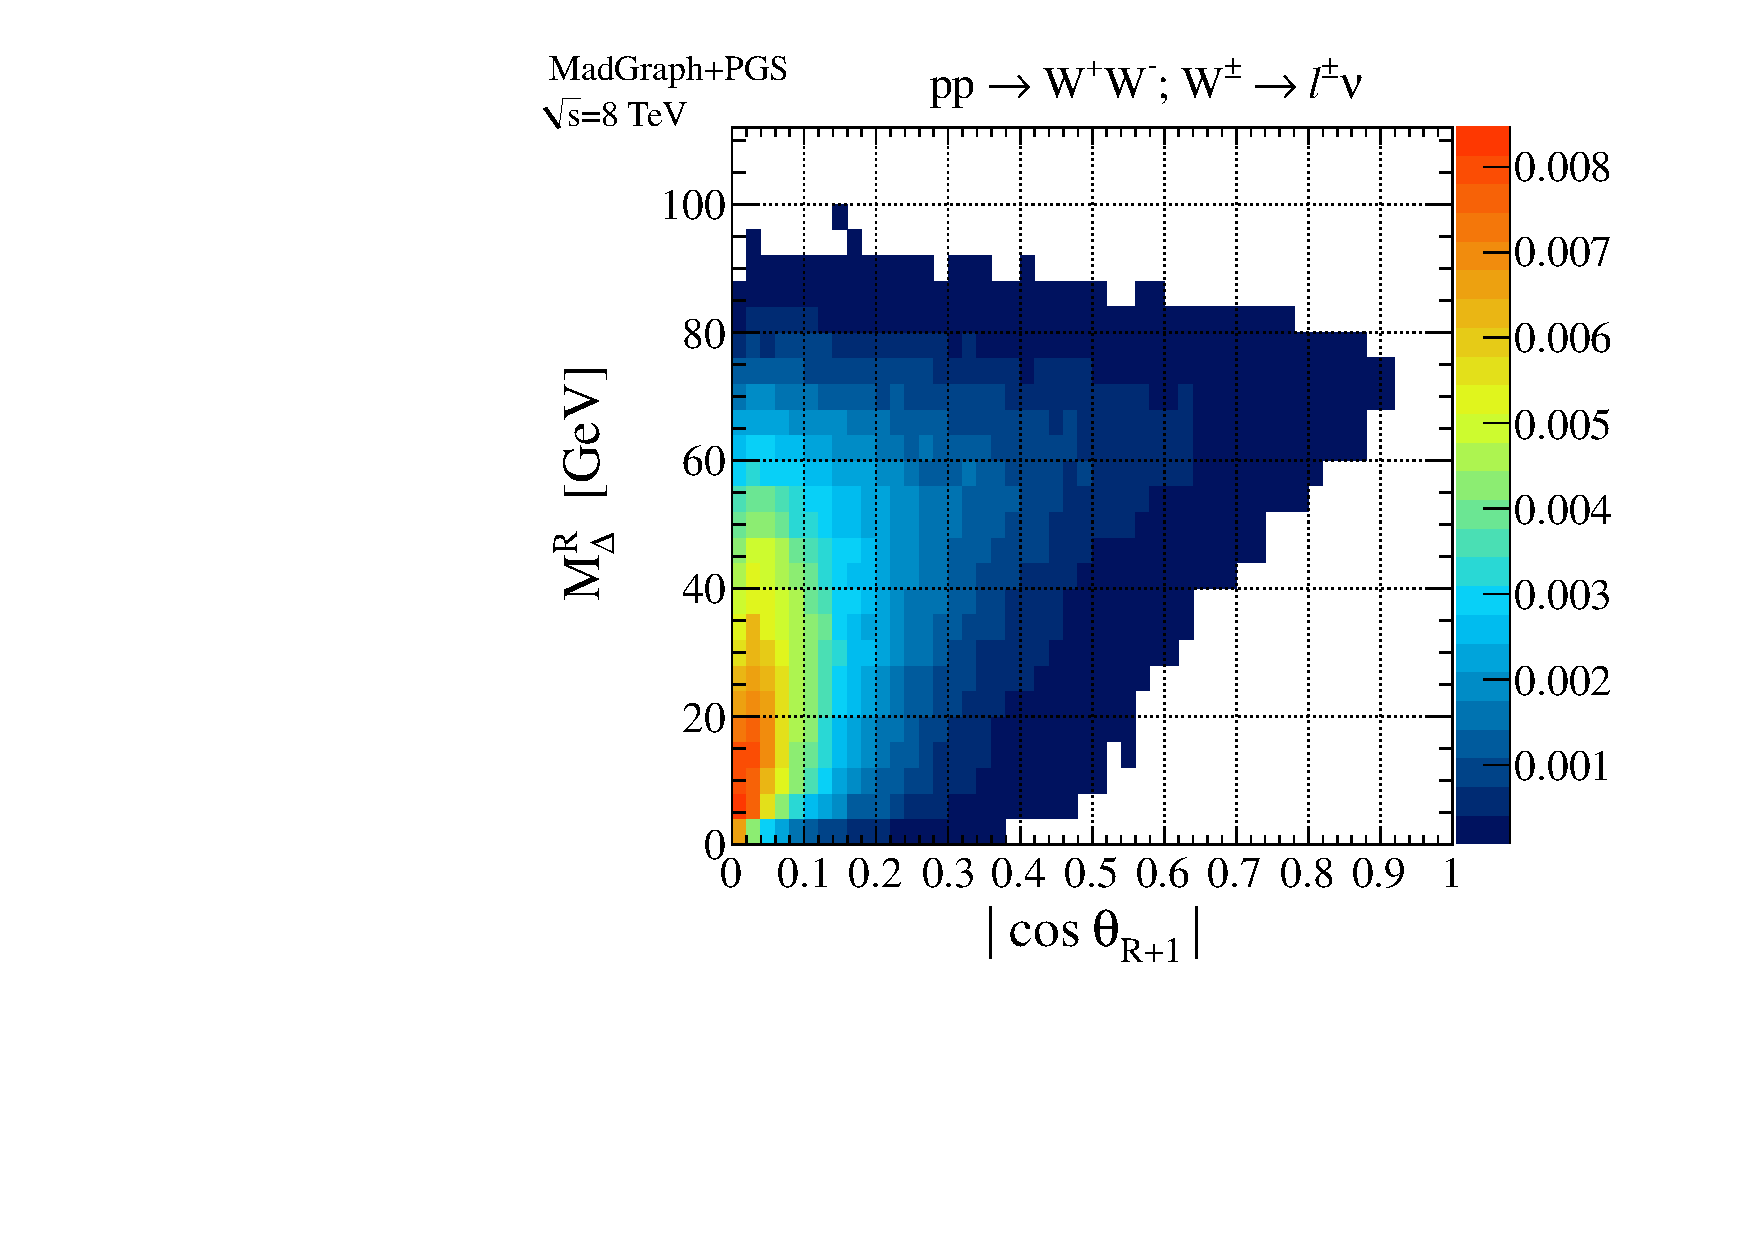
\includegraphics[width=0.35\columnwidth]{fig/sectionII/Mdelta_v_costheta_WW.pdf}
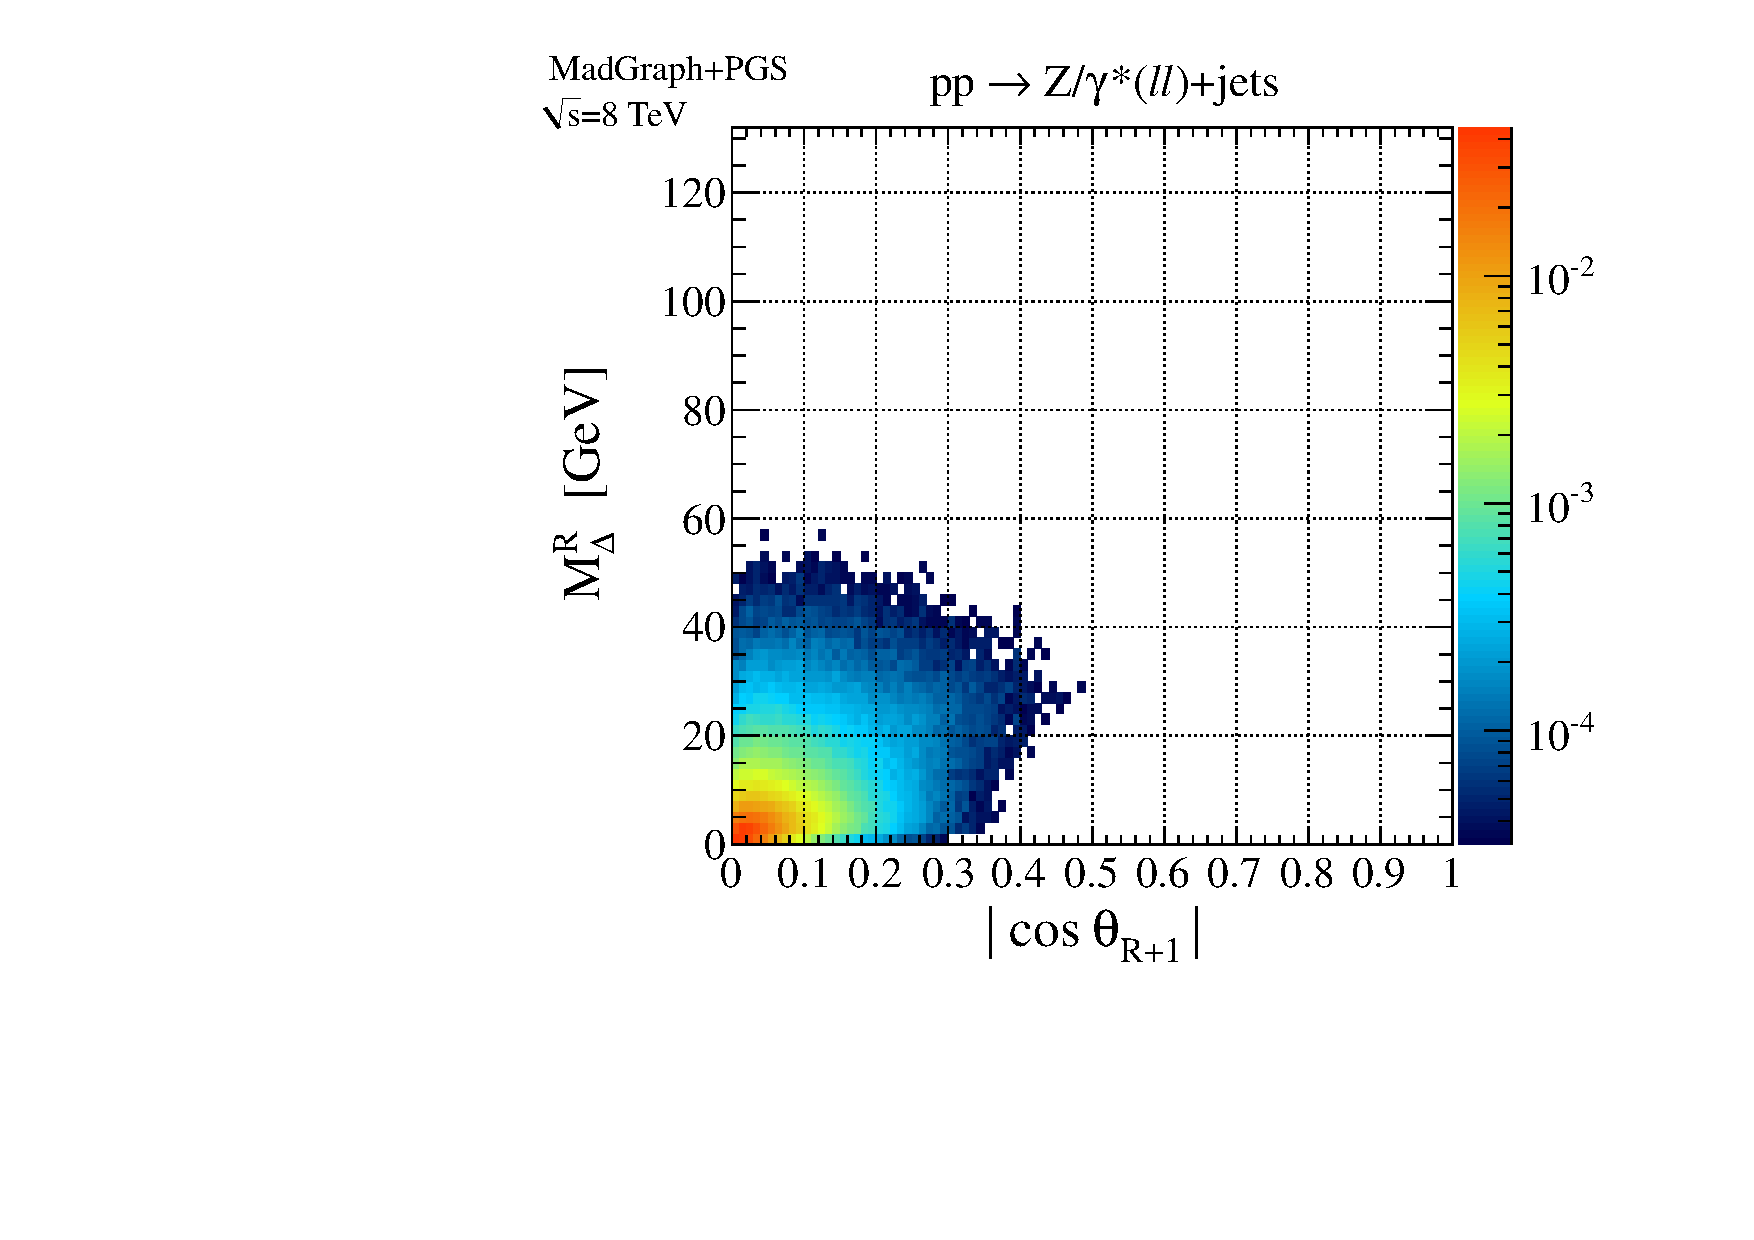
\includegraphics[width=0.35\columnwidth]{fig/sectionII/Mdelta_v_costheta_DY.pdf}
\caption{Upper Row: Distribution of $|\cos\theta_{R+1}|$ versus $M_\Delta^R$ for 150 GeV selectron (left) or chargino (right) pair production, decaying into 50 GeV neutralinos. Lower Row: $|\cos\theta_{R+1}|$ versus $M_\Delta^R$ for $W^-W^+$ pair production (left) or Drell-Yan $Z$ (right) backgrounds decaying into leptons. \label{fig:costheta_v_MdeltaR}}
\end{figure}

\begin{figure}[ht]
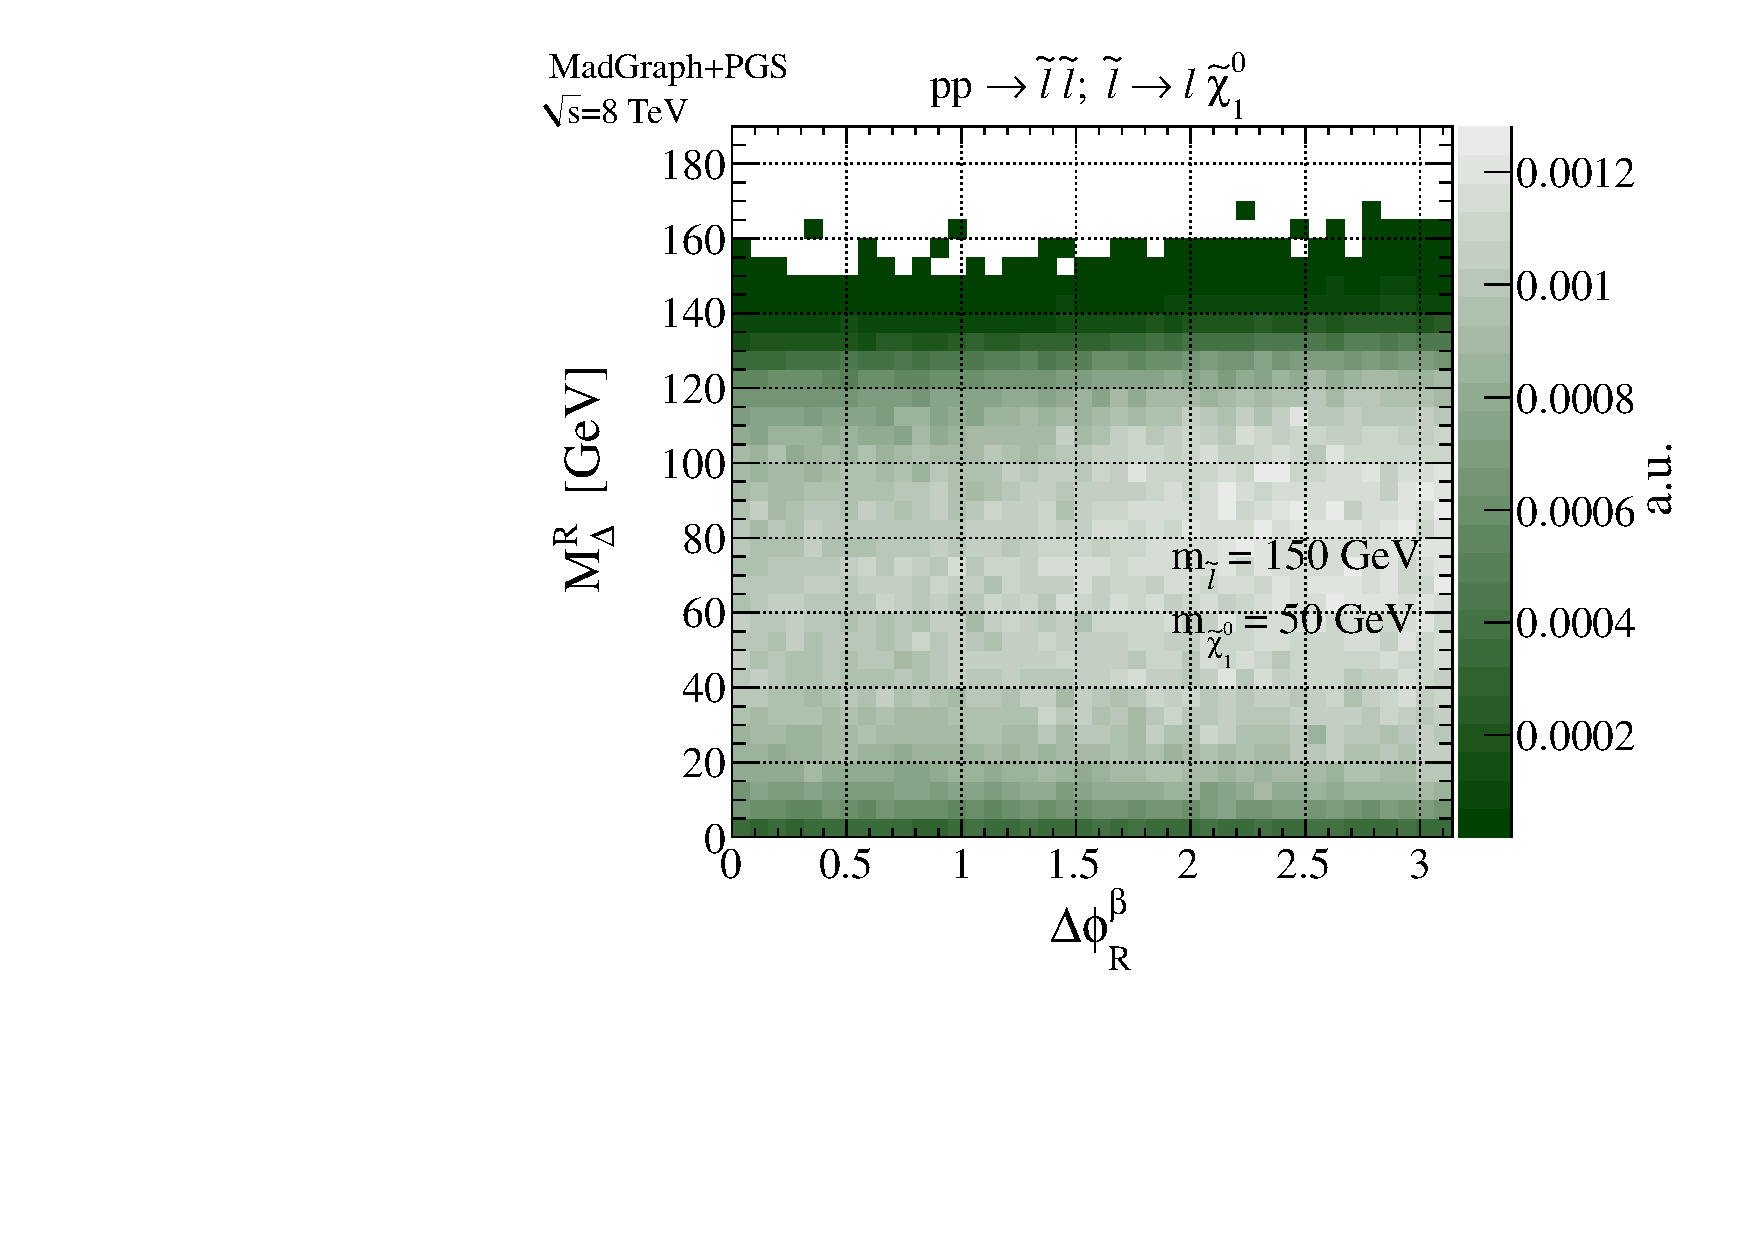
\includegraphics[width=0.35\columnwidth]{fig/sectionII/Mdelta_v_dphi_slepton_150_50.pdf}\includegraphics[width=0.35\columnwidth]{fig/sectionII/Mdelta_v_dphi_WW.pdf}
\includegraphics[width=0.35\columnwidth]{fig/sectionII/costheta_v_dphi_selectron_150_50.pdf}\includegraphics[width=0.35\columnwidth]{fig/sectionII/costheta_v_dphi_WW.pdf}
\caption{Representative distribution of $\Delta\phi_R^\beta$ vs.~$M_\Delta^R$ (top row) and $\Delta\phi_R^\beta$ vs.~$|\cos\theta_{R+1}|$ (bottom row) 
 for 150~GeV selectrons decaying to 50~GeV neutralinos (left) and $W^-W^+$ background (right).  \label{fig:deltaphiMdelta}}
\end{figure}
